\documentclass{article}
\usepackage{array, booktabs, graphicx, apacite, setspace}
\usepackage[titletoc,toc,title]{appendix}
\usepackage[toc,section=section]{glossaries}
\usepackage{tocloft}
\usepackage{titlesec}
\usepackage{fancyvrb}
\usepackage{float} % for strict figure placement  with option [H]
\usepackage[bottom]{footmisc} % to glue footnote to bottom of page
\usepackage{alltt} % for bold typewriter


% set section indentation
\setcounter{secnumdepth}{4}


% add space between paragraphs
\setlength{\parskip}{\baselineskip}


% format \paragraph{example} as a subsubsubsection
\titleformat{\paragraph}
{\normalfont\normalsize\bfseries}{\theparagraph}{1em}{}
\titlespacing*{\paragraph}
{0pt}{3.25ex plus 1ex minus .2ex}{1.5ex plus .2ex}


% automatically convert "" to ``''
\usepackage [autostyle, english = american]{csquotes}
\MakeOuterQuote{"}


% define list of equations
\newcommand{\listequationsname}{\Large{List of Equations}}
\newlistof{myequations}{equ}{\listequationsname}
\newcommand{\myequations}[1]{
   \addcontentsline{equ}{myequations}{\protect\numberline{\theequation}#1}
}
\setlength{\cftmyequationsnumwidth}{2.3em}
\setlength{\cftmyequationsindent}{1.5em}


% format appendix numbering
\renewcommand\appendix{\par
  \setcounter{section}{0}
  \setcounter{subsection}{0}
  \setcounter{figure}{0}
  \setcounter{table}{0}
  \renewcommand\thesection{Appendix \Alph{section}}
  \renewcommand\thefigure{\Alph{section}\arabic{figure}}
  \renewcommand\thetable{\Alph{section}\arabic{table}}
}


% -------- GLOSSARY ENTRIES -------- %
\makenoidxglossaries

\newglossaryentry{word}{
	name={Word},
	description={Definition of the word}
}


% renames "Contents" to "Table of Contents"
\renewcommand\contentsname{Table of Contents}

\begin{document}

% -------------------------------------- %
% ------------ FRONT MATTER ------------ %
% -------------------------------------- %

% -------- TITLE PAGE -------- %

\title{\huge CPEN 411 \\ \Large \medskip Computer Architecture}
\author{Charles Clayton}
\date{\today}
\maketitle
`
\thispagestyle{empty}

\pagenumbering{roman}
\setcounter{page}{0}


% -------- TABLE OF CONTENTS/LISTS -------- %

\singlespacing			\pagebreak
\tableofcontents		\pagebreak

\listoffigures		
\listoftables
\listofmyequations
\pagebreak


% -------- GLOSSARY -------- %

\printnoidxglossaries	\pagebreak


% ----------------------------- %
% -------- MAIN MATTER -------- %
% ----------------------------- %

\pagenumbering{arabic}









\newpage

\section{Fundamentals of Computer Design}

\textbf{Goals of this section}

\begin{enumerate}
\item Determine the high level goals of a computer architect
\item Determine what a simple MIPS64 program computes
\item List instruction processing steps in the von Neumann architecture
\item Describe how technology trends impact latency and bandwidth
\item Analyze how active and static power change as voltage and clock frequency change
\item Define cost, price, and explain their trends
\item Demonstrate how to measure and report performance
\item Define several quantitative principles and apply them
\item Explain some common pitfalls and fallacies
\end{enumerate}

\subsection{Tasks of the Computer Designer}

A computer designer must coordinate the many levels of abstraction under rapidly changing sets of pressures, including technology, applications, history, and to lesser extent operating systems and programming languages. Additionally, they must be able to measure and evaluate their designs.

\subsubsection{Make the Common Case Fast}

If a task is repeated or done frequently, this is the task that should be optimized. 

\subsubsection{Take Advantage of Parallelism}

Parallelism is exploited in modern microprocessors. We will explore how this is done later. The levels of parallelism are

\begin{enumerate}
\item \textbf{Thread level parallelism, TLP} -- independent programs on different processors

\item \textbf{Data level parallelism, DLP} -- multiple instances of the same program on different input data

\item \textbf{Instruction level parallelism, ILP} -- multiple instructions simultaneously executed

\item \textbf{Parallel digital circuits} -- different parts of a digital circuit operating in parallel during same clock cycle
\end{enumerate}

\subsubsection{Principle of Locality}

Programs tend to reuse data and instructions that they have used recently, in other words, a program spends 90\% of its time in 10\% of its code. That means we can predict what instructions and data a program will likely use.

\subsubsection{Amdahl's Law}

\textbf{Amdahl's law} describes whether to develop parallel processors. Since there will be a portion of the code that cannot be parallelized, it's important to focus on a single processor. 

\begin{equation}
Speedup_{overall} = \frac{ExTime_{old}}{ExTime_{new}} = \frac{1}{1-Fraction_{enhanced} + \frac{Fraction_{enhanced}}{Speedup_{enhanded}}}
\end{equation}
\myequations{Amdahl's Law}


\begin{equation}
Speedup_{maximum} = \frac{1}{1-Fraction_{enhanced}}
\end{equation}
\myequations{Maximum speedup}

\begin{equation}
Speedup_{overall} = \frac{1}{1-Fraction_{1}-Fraction_2 + \frac{Fraction_{1}}{Speedup_{1}} + \frac{Fraction_2}{Speedup_2}}
\end{equation}
\myequations{Amdahl's Law with Multiple Optimizations}

\subsubsection*{Example}

20\% of the execution time is due to floating point square root operations, and 50\% of the execution time is due to \textit{all} floating point operations. Would it be better to speed of FPSQR by a factor of 10, or speed up all FP operations by a factor of 1.6?

---

$$
SU_{FPSQR} = \frac{1}{1-0.20 + \frac{0.20}{10}} = 1.2195 \rightarrow 21.95\%\ faster
$$

$$
SU_{FP} = \frac{1}{1-0.50 + \frac{0.50}{1.6}} = 1.2308 \rightarrow 23.08\%\ faster
$$

So you get more speedup by increasing all floating point operations by 1.6

\subsubsection*{Example}

There are three possible enhancements you may do. $SU_{1} = 30$, $SU_2 = 20$, $SU_3 = 15$. If $E_1$ and $E_2$ are each usable 25\% of the time, what fraction of the time must $E_3$ be used to achieve the overall speedup of 10.

---

$$
10 = \frac{1}{1 - 0.25 - 0.25 - E_3 + \frac{0.25}{30} + \frac{0.25}{20} + \frac{E_3}{15}} \rightarrow E_3 = 0.45
$$

\subsubsection{The Iron Law of Processor Performance}

Execution time is the only real measure of performance because frequency and parallelism and so on all amount to this. Many instructions take different numbers of cycles, so in order to determine the execution time, we calculate the total execution time from instruction count, cycles per instruction, and the cycle time.

\begin{equation}
Execution\ time = \frac{1}{Performance} = (Inst.\ count)(CPI)(Cycle\ time)
\end{equation}
\myequations{Iron Law of Processor Performance (Execution time)}

Cycles per instruction, \textbf{CPI}, is the average number of cycles per instruction across all instructions executed by a program. Typically $CPI < 1$ because of parallelism, but should approximately be around 1. 

The CPU Time is the total amount of time for a sequence of instructions. Where $I_j$ is the instruction count and $CPI_j$ is the cycles per instruction for instruction $j$.

\begin{equation}
CPU\ Time = Cycle\ time \times \sum\limits_{j = 1}^n (CPI_j)(I_j)	
\end{equation}
\myequations{CPU Time}

\subsubsection*{Example}

You consider optimizing one of your instructions. You implement your processor both "with" and "without" this optimization and measure the following.

$$
\begin{matrix}
 Cycle\ time_{with} = (1.05)(Cycle\ time_{without}) \\
 IC_{with} = (0.99)(IC_{without})  \\
 CPI_{with} = (1.01)(CPI_{without}) \\
\end{matrix}
$$

Should you use the optimization?

---

$$
\begin{matrix}
Execution\ time_{with} = 1 \times 1 \times 1 = 1 \\ 
Execution\ time_{without} = (1.05)(0.99)(1.01) = 1.05 \\ 
\end{matrix}
$$

The execution time with the optimization is smaller, so we should use the optimization.

\subsection{Computer Performance}

CPI, instruction count, and cycle time are often improved as a tradeoff. Designers have run out of steam as far as increasing processor frequency to reduce cycle time, since power limitations have reduced the returns by increasing frequency.

\subsubsection{How to Measure CPI}

There are three ways of running simulations to estimate CPI when designing a microprocessor. 

\begin{enumerate}
\item \textbf{Functional simulator} -- these emulate one instruction at a time, then measure the number of cycles each, and are not very accurate
\item \textbf{Performance simulator} -- these create a timing model to capture when stalls occur, they have an accuracy within 5-10\% but are the most used for design exploration
\item \textbf{RTL (register-transfer level) model} -- these model the circuit with an HDL and give a very precise measure of CPI, but are very slow
\end{enumerate}

\begin{figure}[ht!]
\centering
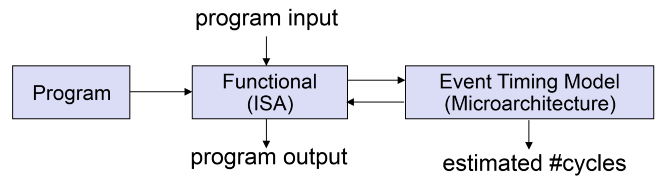
\includegraphics[width=80mm]{img/PerformanceSimulator.png}
\caption{Performance simulator}
\end{figure}

\subsubsection{Metrics of Performance}

Performance is measured in different metrics for different applications. For instance, google's metrics are probably something like searches/hour. In our case, you will see metrics such as \textbf{MIPS} (millions of instructions per second) and \textbf{MFLOP/s} (millions of FP operations per second). At ever lower levels, in the database it would be Gb transmitted per second, and at the circuit level it would be cycles per second.

However, these are mostly "marketing numbers", the only consistent measurment is total execution time.

Since we want to treat performance as numbers that get larger the better they are, we take performance to equal

\begin{equation}
Performance = \frac{1}{Execution\ time}
\end{equation}

So when we say "$X$ in $n$ times faster than $Y$" or "Speedup of $X$ compared to $Y$ is $n$", that means

\begin{equation}
n = \frac{Performance\ X}{Performance\ Y}
\end{equation}

\subsubsection{Evaluating Performance}

We often evaluate processor performance through \textbf{benchmarks} -- applications that are representative of programs that will be run on our architecture. Most benchmarks are \textbf{kernels}, which are small pieces of code from real programs. A famous kernel is Linpack, which is a linear algebra and runs mostly matrix operations, operations highly used by applications such as games and photoshop.

Good benchmarks do not take too long to simulate, are not too application specific, and are not so large that it is hard to identify the location of performance losses.

Academics formed some standardized \textbf{benchmark suites} so that different companies architecture can be compared in a stable and consistent way. They are a collection of applications indicative of a variety of uses to measure the overall performance of a computer.

 \textbf{SPECCint CPU2006} and previous versions of SPEC are the most widely used benchmark suites. They include applications for compression (gzip), compilation (gcc), and interpretation (perl) as well as many others. These change every few years, because the benchmarks need to be standardized, but also most evolve with the typical computer uses.
 
\subsubsection{Comparing and Summarizing Performance}


There are multiple ways to quantify performance

\begin{enumerate}
\item \textbf{weighted execution time} -- depends on how much each computer uses each specific application being tested
\item \textbf{arithmetic mean} -- can change depending on which computer you choose to make as your baseline

\item \textbf{geometric mean} -- shows the best performing machine regardless of baseline and is used by SPEC, however it does not predict execution time
\end{enumerate}

\begin{equation}
Geometric\ mean = \sqrt[n]{\prod_{i=1}^{n} Execution\ time\ ratio_{i}}
\end{equation}
\myequations{Geometric mean}

An alternative to the geometric mean is the \textbf{harmonic mean} which gives more weight to smaller differences because it takes the inverse of the data. It is up for debate which is better.

\begin{equation}
Harmonic\ mean = \frac{n}{\sqrt[n]{\prod_{i=1}^{n} \frac{1}{Execution\ time\ ratio_{i}}}}
\end{equation}
\myequations{Harmonic mean}

The harmonic mean $\le$ geometric mean $\le$ arithmetic mean.

\subsubsection*{Example}

Computer A executes program P1 in 1 second, and program P2 in 1000 seconds. Computer B executes P1 and P2 in 10 and 100 seconds respectively, and computer C, 20 seconds and 20 seconds. Which computer is fastest according to the geometric mean?

--- 

Let computer A be the baseline, since choosing any computer as the baseline will yield the same result. So $geometric\ mean_A = \sqrt{\frac{1}{1} \times \frac{1}{1}} = 1$. 

For computer B, $geometric\ mean_B = \sqrt{\frac{P1_B}{P1_A} \times \frac{P2_B}{P2_A}} =  \sqrt{\frac{10}{1} \times \frac{100}{1000}} = 1$


For computer C, $geometric\ mean_C = \sqrt{\frac{P1_C}{P1_A} \times \frac{P2_C}{P2_A}} =  \sqrt{\frac{20}{1} \times \frac{20}{1000}} = \textbf{0.632}$

Since the geometric mean of computer C, is the smallest, computer C is the fastest. See Figure 2 to compare the geometric mean to the arithmetic mean.

\begin{figure}[ht!]
\centering
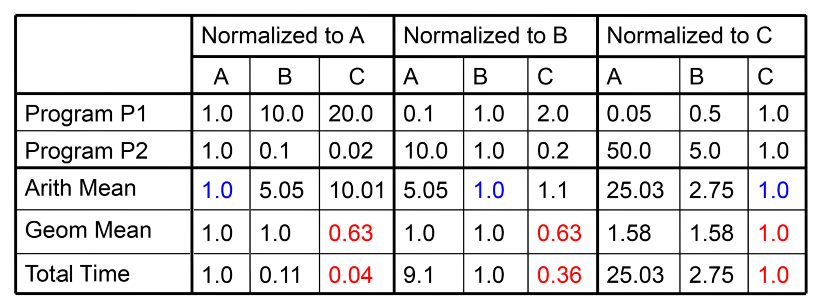
\includegraphics[width=110mm]{img/ArithGeo.png}
\caption{Arithmetic Mean vs. Geometric Mean}
\end{figure}

\subsubsection{Power}

Power is the most restrictive factor and has dominated the constraints for high performance, especially in mobile devices. 

There are two kinds of power consumption:

\begin{enumerate}
\item \textbf{Dynamic power} -- Losses when switching transistors between high and low, which causes some current to flow, and transistors/wires have nonzero capacitance

\item \textbf{Static power} -- Due to leakage current flow from the transistor, even when it is not switching between high and low

\end{enumerate}

Historically, static power losses has been negligible in comparison to dynamic power, but static power has increased significantly in recent years because there are so many more transistors on a device, thus there is more leakage, and in addition, the transistors are smaller which means more leakage. The goal for static power is round 25\% of total power consumption, and up to 40\% for high performance systems.

With high performance systems, such as desktops and servers, we are mostly concerned with the \textit{power} losses. The capacitance is a function of the number of transistors, and of the technology (smaller transistors having lower capacitance). 

\begin{equation}
P_{dynamic} = \frac{1}{2}C V^2 f
\end{equation}
\myequations{Dynamic power losses}

Dynamic power is obviously dependent on voltage as a square, but voltage and frequency are actually directly related as well, so power is related to voltage as a cubic. 

A high voltage system means that there is less delay due to capacitance when switching a transistor, so you can operate at a higher frequency. This is why you must increase the voltage supply when overclocking a chip. 

By decreasing the voltage (as has been done in recent years), the maximum frequency has decreased, and the power consumption has also decreased.

With mobile devices, \textit{energy} is a better metric. 

\begin{equation}
E_{dynamic} = CV^2
\end{equation}
\myequations{Dynamic energy losses}

Slowing the clock rate reduces power consumption, but not energy. This is slightly counter-intuitive, but imagine yourself lifting a weight. If you lift the weight from 2ft to 4ft, the amount of energy (work) done is the same no matter how fast you do it because you've only increased the potential energy by 2ft. However, the power (rate of work) exerted is higher the faster the weight is lifted.

So for a given computation, by decreasing the frequency of the chip, you will use less power, but you will use the same amount of energy.

\subsubsection*{Example}

Suppose a 15\% reduction in frequency (reducing performance by roughly the same amount) allows us to safely reduce voltage by 15\%. What is the impact on dynamic power?

---

\begin{align*}
  P_{old}  =\ & \dfrac{1}{2} C V^2 f = 0.5  \\
  P_{new} =\ & \dfrac{1}{2} C ((1-0.15)V)^2 (1-0.15)f = 0.307 \\
  \%\ change =\ & \dfrac{0.307-0.5}{0.5}100\% = -38.6\%
\end{align*}

There was about a 40\% reduction in dynamic power consumption. 

\subsection{Integrated Circuits Cost}

When producing wafers, there will be defects in some so only a percentage of them  will be usable, this is called the \textbf{wafer yield}. Unless it is given, assume the wafer yield in 100\%, realistically it is more like 98\%. Furthermore, when creating dies from the wafers, some dies will have too many defects to be usable. The percentage of usable dies is the \textbf{die yield}.

\begin{equation}
IC\ cost = \dfrac{Die\ cost + Testing\ cost + Packaging\ cost}{Final\ test\ yield}
\end{equation}
\myequations{IC Cost}

\begin{equation}
Die\ cost = \dfrac{Wafer\ cost}{Dies\ per\ wafer * Die\ yield}
\end{equation}
\myequations{Die cost}

\begin{equation}
Dies\ per\ wafer = \dfrac{\pi (Wafer\ radius)^2}{Die\ area} - \dfrac{2\pi * Wafer\ radius}{\sqrt{2 * Die\ area}} - Test\ die
\end{equation}
\myequations{Dies per wafer}

Alpha $\alpha$, is a technology-dependent factor. Unless it is provided, assume it is one.

\begin{equation}
Die\ yield = Wafer\ yield \left(1 + \dfrac{Defect\ density * Die\ area}{\alpha}\right)^{-\alpha}
\end{equation}
\myequations{Die yield}

\begin{equation}
Test\ cost = \frac{Hourly\ cost * Test\ time}{Die\ yield}
\end{equation}
\myequations{Testing cost}

It's interesting to note, that for instance an i7 core is actually the same die as an i5 core. An i5 core is just an i7 core with extra defects, and intel may have just turned off a couple additional features through firmware. 

\subsubsection*{Example}

What is the cost of producing dies if the defect density is $0.3/cm^2$ vs. $1.0/cm^2$ and provided the following specs.

\begin{align*}
\alpha 			=&\	 4 \\
Die\ area 		=&\	 300mm^2 \\
Wafer\ diameter =&\	 200mm \\  
Wafer\ yield 	=&\	 0.95 \\
Pins 			=&\	 418 \\
Technology 		=&\	 CMOS, 0.18um, 6M \\
Wafer\ cost 	=&\	 \$4900 \\
Package 		=&\	 \$20 \\
Test\ time 		=&\	 30 sec \\
Test\ cost 		=&\	 \$400/hr \\
Final\ test\ yield =&\ 1.0 
\end{align*}

---

$$
Dies\ per\ wafer = \dfrac{\pi (100mm)^2}{300mm^2} - \dfrac{2\pi * 100mm}{\sqrt{2 * 300mm^2}} = 79
$$

$$
Die\ yield_{0.3} = 0.95 \left(1 + \dfrac{(0.3/cm^2)(300mm^2)}{4}\right)^{-4} = 42.19\%
$$

$$
Die\ cost_{0.3} = \dfrac{\$4900}{79(0.4219)} = \$147
$$

$$
Test\ cost_{0.3} = \frac{\$400/hr * 30 \frac{1 hr}{3600sec}}{0.4219} = \$7.90
$$


$$
Total\ cost_{0.3} = 147 + 7.90 + 20 = \textbf{\$174.90}
$$

When the process is repeated for the $1.0/cm^2$ defect density, you get a die yield of $10.13\%$, a die cost of $\$612.50$, a testing cost of $\$32.91$, and thus a total cost of $\textbf{\$665.41}$.

\subsection{Technology Trends}

When transistors get smaller, they are less capacitive and thus can switch faster, so the frequency can be increased. Additionally, smaller transistors require less voltage. And finally, smaller transistors mean more available space on the chip. So you can get drastic performance improvements simply by making transistors smaller, and up until the end of Moore's law, much of EE was focused on doing just that.




\subsection{Levels of Representation}

A high level programming language is compiled into assembly language, which is then assembled into machine code. 


$\texttt{int a = 10;}\ \rightarrow\ \texttt{LW R15, 0(R2)}\ \rightarrow\ \texttt{1000 1100 0010 0000 0000 0000 0000} $

The machine code includes the control bits, which the machine must extract to determine the instruction, and it includes the data bits, which indicate where the data comes from. 

\subsubsection{Fundamental Execution Cycle}

In order for the computer to process and run any instruction, it must go through the instruction cycle. Each step here is referred to as a phase. It must first \textbf{fetch the instruction}, \textbf{decode} the instruction, \textbf{fetch the operands}, \textbf{execute}, \textbf{store} the result, and determine \textbf{next instruction}. See figure 3.


\begin{figure}[ht!]
\centering
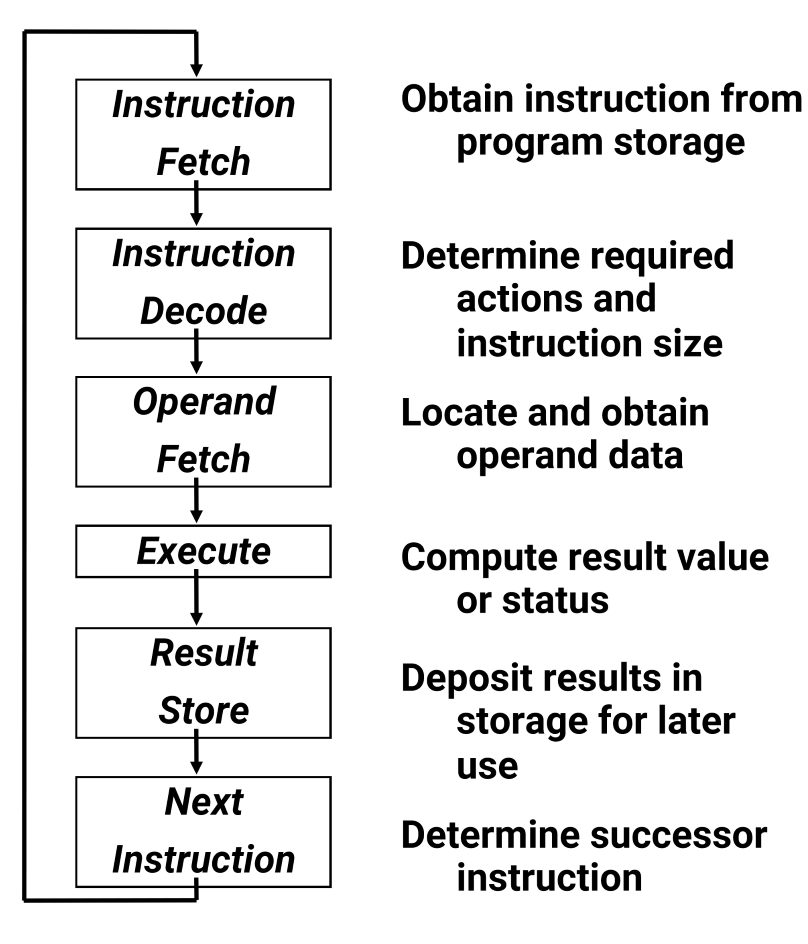
\includegraphics[width=60mm]{img/InstructionCycle.png}
\caption{Instruction Cycle}
\end{figure}

 The instruction fetch of the next instruction, may or may not depend upon the result of the previous instruction.

\subsection{MIPS}

This is the language that is the focus of the course. It is a very clean architecture, and an example of a well-designed language. 

All the instructions are the same size, and thus the program is easy to decode. It uses the load-store architecture, meaning that all arithmetic is register-to-register. Some languages can have functions such as "add register 5 to memory location 17", but MIPS does everything with registers. This separates memory from computations. MIPS also maximizes its hardware reuse. 

In many processors, even the x86 instruction set is recompiled into $\mu$ops, which is a language very similar to MIPS. x86 is maintained largely in order to provide legacy support.

MIPS is a RISC (Reduced Instruction Set Computer) instruction set architecture. One of the first modern architectures was the PentiumPro, which had a CISC (Complex Instruction Set Computer) ISA, and could execute instructions out-of-order, speculatively. This was around the mid '90s.

\subsubsection{Example MIPS64 Instructions}

\begin{table}[ht]
  \centering
  \caption{Example MIPS ALU Instructions}
  \begin{tabular}{
  		>{}m{1.3in} 
  		>{}m{1.5in} 
  		>{}m{1.7in}
  		}
    \toprule
    \textbf{Instruction} & \textbf{Description} & \textbf{Meaning}  \\ 
    \midrule
	\texttt{DADDU R1, R2, R3} & Add unsigned &  R1 = R2 + R3	\\
		\texttt{DADDIU R1, R2, \#3} & Add immediate unsigned &  R1 = R2 + 3	\\
	\texttt{LUI R1, \#42} & Load upper immediate & R1 =  $0^{32}$...42...$0^{16}$ 	\\
	\texttt{DSLL R1, R2, \#5} & Shift left logical &  R1 = R2 $\ll$ 5	\\
	\texttt{DSLT R1, R2, R3} & Set less than &  R1 = R2 $<$ R3 ? 1 : 0 $\ll$ 5	\\

	\bottomrule
  \end{tabular}
\end{table}

\begin{table}[ht]
  \centering
  \caption{Example MIPS Load/Store Instructions}
  \begin{tabular}{
  		>{}m{1.1in} 
  		>{}m{1.2in} 
  		>{}m{2.1in}
  		}
    \toprule
    \textbf{Instruction} & \textbf{Description} & \textbf{Meaning}  \\ 
    \midrule
	\texttt{LD R1, 30(R2)} & Load double word &  R1=Mem[30+R2] ... Mem[30+R2]	\\
		\texttt{LW R1, 60(R2)} & Load word & R1=Mem[60+R2]	\\
	\texttt{SW R3, 500(R4)} & Store word & Mem[500+R4] = R3	\\
	\texttt{L.S F0,50(R3)} & Load FP single &  R0 = Mem[50+R3] ... $0^{32}$	\\
	\texttt{L.D F0, 50(R2)} & Load FP double &   F0 = Mem[50+R3]	\\

	\bottomrule
  \end{tabular}
\end{table}


\subsubsection{Branches}A branch is a way of jumping over code. For instance, the conditional \texttt{if} statement in the following C code is converted to the MIPS branch \texttt{BEQZ}.

\singlespacing
\begin{Verbatim} 
	x = 0;				DADDI R1, R0, \#0
	if(p != NULL)			 BEQZ R2, target
    	x = *p;			   LD R1, 0(R2)
	*q = x;		       target: SD R1, 0(R3)

\end{Verbatim}

\begin{table}[ht]
  \centering
  \caption{MIPS Control Flow Instructions}
  \begin{tabular}{
  		>{}m{1.2in} 
  		>{}m{1.5in} 
  		>{}m{1.8in}
  		}
    \toprule
    \textbf{Instruction} & \textbf{Description} & \textbf{Meaning}  \\ 
    \midrule
	\texttt{J name} 	& Jump             			& PC = name 	\\
	\texttt{JAL name} 	& Jump and link    			& R31 = PC + 4; PC = name; \\
	\texttt{JALR R2} 	& Jump and link register 	& R31 = PC + 4; PC = R2; \\
	\texttt{JR R3} 		& Jump register 	 		& PC = R3 \\
	\texttt{BEQZ R4, name} 		& Branch equal zero & if (R4 == 0) PC = name \\
	\texttt{BNE R3, R4, name} 	& Branch not equal  & if (R3 != R4) PC = name \\
	\texttt{MOVZ R1, R2, R3} 	& Conditional move if zero  & if (R3 == 0) R1 = R2 \\

	\bottomrule
  \end{tabular}
\end{table}

\subsubsection{Instruction Encoding}

Encoding is how we represent an instructions as ones and zeros for the computer to interpret. All MIPS64 instructions are 32 bits wide and perform simple operations. MIPS divides instructions into three categories.

\begin{enumerate}
\item \textbf{R-type} -- register type instructions, of the form \texttt{OP rs, rt, rd}. Rd represents the destination register, and rt and rs are the two source registers. Additionally, shamt represents a shift amount that can be used with shift and rotate instructions.

\begin{figure}[ht!]
\centering
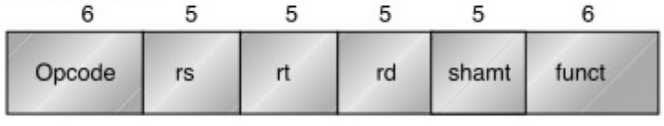
\includegraphics[width=80mm]{img/Rtype.png}
\caption{R-type encoding}
\end{figure}


\item \textbf{I-type} -- immediate type instructions, of the form \texttt{OP rs, rt, IMM}. Here, rt represents the destination register, rs represents the source register, and IMM represents some hard-coded value.

\begin{figure}[ht!]
\centering
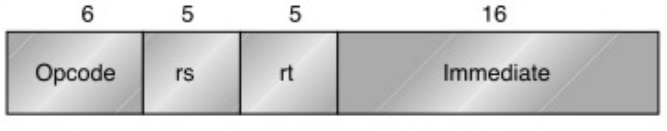
\includegraphics[width=80mm]{img/Itype.png}
\caption{I-type encoding}
\end{figure}

\item \textbf{J-type} -- jump type instructions, of the form \texttt{OP LABEL}, where LABEL is the target address to jump to.
\end{enumerate}

\begin{figure}[ht!]
\centering
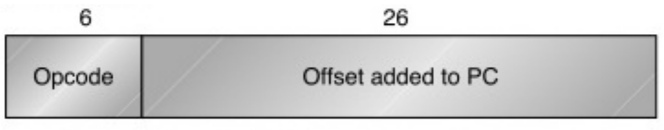
\includegraphics[width=80mm]{img/Jtype.png}
\caption{J-type encoding}
\end{figure}

The funct space is used in addition to opcode to make extra bits available to you.

Note that the order of the registers in the encoded machine code is different from that of the assembly code. Consider the following line of assembly: 

 \texttt{DADD R1, R2, R3}

Which when encoded looks like this:

\begin{figure}[ht!]
\centering
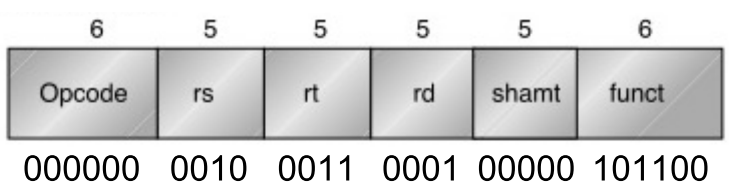
\includegraphics[width=80mm]{img/TranslatedInto.png}
\end{figure}

Observe the source registers are R2 and R3, and the destination register is R1, which is not in the same order the arguments are provided in the MIPS code.

\subsubsection{Registers}

There are 32 general-purpose 64-bit registers, R0--R31. R0 is always 0, and assignments to R0 are ignored. Additionally, there are 32 floating-point registers, F0--F31, that are either 32 of 64-bits.

The PC (Program Counter) is a register that points to the next instruction to be executed. When a jump instruction is made, the PC is modified to be the address of the label. Otherwise, every execution cycle the PC is incremented by 4 bytes, because each MIPS instruction is 32 bits, so the PC points to the next instruction in memory.

\subsubsection{Memory}

The 32 general purpose registers are not enough to store the information needed for most programs. 32 registers can all be identified using 5 bits in the instruction encoding space, increasing the number of registers increases this valuable space. Additionally, registers take up more space and use more power. However, some registers are valuable because that can be written to and read from extremely fast and reduce the number of memory operations.

So on top of registers, all computers have random access memory  (RAM) to store data. All instructions are stored in memory. To retrieve data, you must know its address in the memory. 

\subsubsection{Elements of an ISA}

\begin{enumerate}

\item Set of machine-recognized data types -- bytes, words, integers, FP, strings...

\item Operations performed on those data types -- add, sub, mul, xor, move...

\item Programmable storage -- registers, PC, RAM...

\item Method of obtaining data referenced by instructions

\item Format (encoding) of the instructions -- op codes, operand fields

\end{enumerate}


\subsubsection{ISA Classes}

There are four distinctly different instruction set classes. Let's observe how each class would compute$C = A + B$.

\begin{enumerate}

\item \textbf{Stack} -- Like an HP-50g. It has good code density, but is hard to reorder instructions, and requires extra code/memory bandwidth. 

\begin{Verbatim}
Push A
Push B
Add
Pop C
\end{Verbatim}

\item \textbf{Accumulator} -- This class only has one register. It has very small instruction encoding, good code density, but it difficult for the compiler. 

This class has the most dense encoding. It requires the fewest bits of storage to represent the assembly code.


\begin{Verbatim}
Load A
Add B  ; to whatever is in the one register
Store C
\end{Verbatim}


\item \textbf{Register-Memory} -- This can do operations both from registers and memory. It usually has a limited number of registers.


\begin{Verbatim}
Load R1, A
Add R3, R1, B
Store R3, C
\end{Verbatim}


\item \textbf{Register-Register} -- Like MIPS. Operations can not be done on memory, only registers. This requires more registers, and has poor code density (more instructions to do the same thing). 

However, the main reasons we use this is because it is easy to pipeline, and easy for the compiler to generate efficient code.


\begin{Verbatim}
Load R1, A
Load R2, B
Add R3, R1, R2
Store R3, C
\end{Verbatim}


\end{enumerate}

\begin{figure}[ht!]
\centering
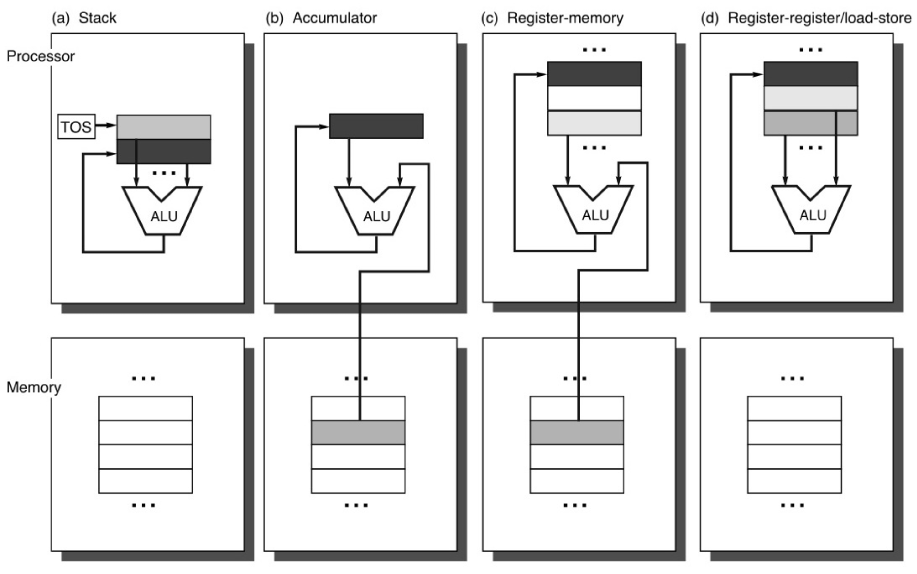
\includegraphics[width=90mm]{img/ISAClasses.png}
\caption{ISA Classes}
\end{figure}

\subsubsection{Memory Addressing}

Data values are stored in memory at a location determined by the memory address. 

\textit{Byte-addressable} memory specifies a multiple of 1-byte in sizes of 8-bits, 16-bits, 32-bits, and 64-bits. \textit{Word-addressable} memory specifies the number of bits used an arithmetic operations, and can be sizes such as 8-bits, 16-bits, and 24-bits. 

Word-addressable requires extra computation, and although is "nice and clean", is not used as much as byte-addressing. 

With \textit{Little Endian}, the least significant (littlest) bit is stored at the beginning (rightmost) of the memory. With \textit{Big Endian}, the most significant (biggest) bit is stored at the beginning of the memory.

\begin{figure}[ht!]
\centering
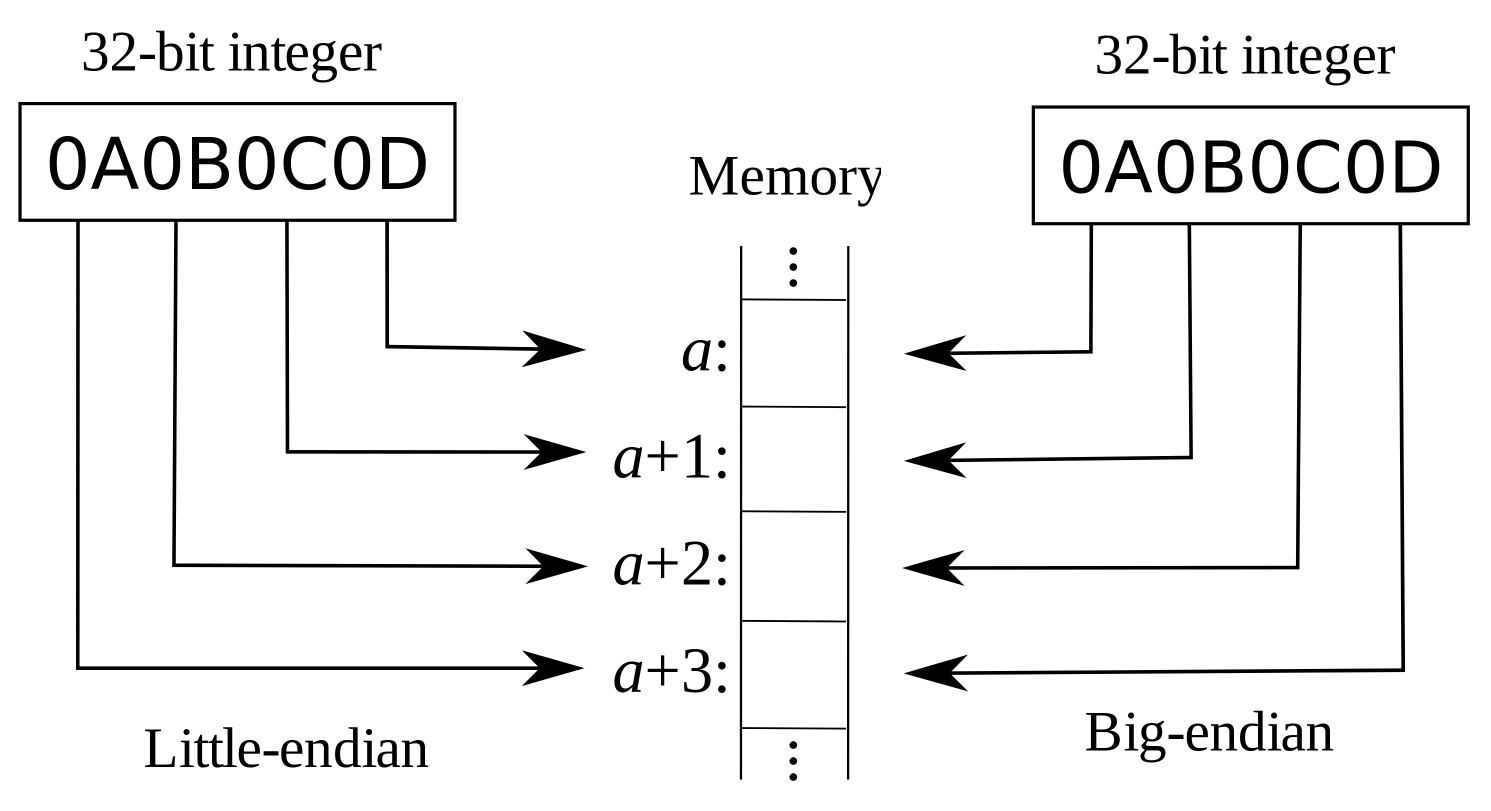
\includegraphics[width=80mm]{img/Endian.png}
\caption{Big vs. Little Endian}
\end{figure}

In practice, most processors use Little Endian. That means if the 4-byte value \texttt{0x12345678} is stored at address \texttt{1000}. Then the value at address \texttt{1011} is \texttt{0x12}.

\subsubsection{Memory Alignment}

In many architectures, particularly RISC architectures, addresses must be aligned. Assume the hardware stores memory in rows of 8-bytes. These rows will be broken up into objects of bytes, half-words (2 bytes), words (4 bytes), and double words (8 bytes). 

When these objects are aligned in memory, they can be retrieved with a single memory access. When data is misaligned, it takes multiple memory accesses to retrieve the data.

 This means that $(Byte\ address)\ mod(Length\ in\ bytes) = 0$.


\begin{figure}[ht!]
\centering
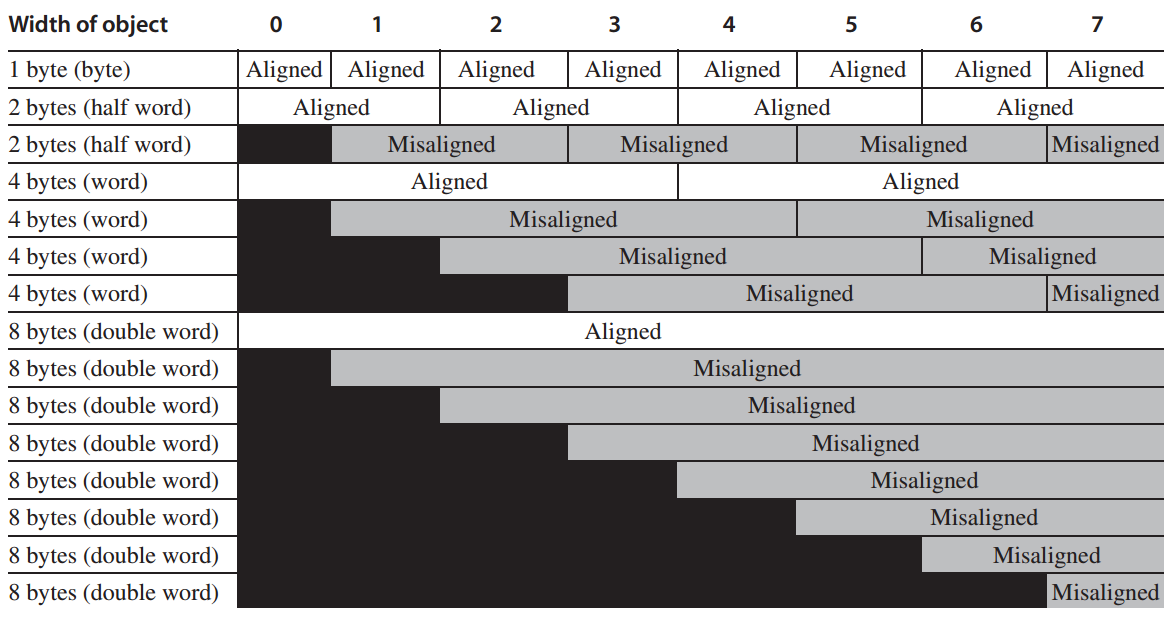
\includegraphics[width=110mm]{img/MemoryAlignment.png}
\caption{Memory Alignment}
\end{figure}




\subsubsection*{Example}

Imagine a RISC instruction set that supports a 24-bit displacement field and that initially Regs[R1]=0x40. We have a program with the following instruction

\texttt{LD R2, 0x10002(R1)}

\noindent How can you implement the same operation using a 16-bit displacement?

---

This instruction stores \texttt{0x10002+0x40=0x100042} in the register R2. This can be achieved with the following:

\begin{verbatim}
LUI R3, #1        ; Regs[R3] = 0x1 << 16 = 0x10000
DADD R4, R3, R1   ; Regs[R4] = 0x10000+0x40 = 0x100040
LD R2, 2(R4)      ; Regs[R2] = 0x10040+0x2 = 0x10042
\end{verbatim}

---

\subsubsection*{Example}

Assuming any size displacement is allowed, a program contains 25\% loads with 50\% of these loads having displacement of 8-bits or less and all loads have displacement of 16-bits or less. 

\textbf{1. }If we require length of load to be \texttt{16+displacement size} bits, which of the following uses less instruction memory: \textbf{(a)} 8-bit or \textbf{(b)} 16-bit displacements for loads (assuming all other instructions are 16-bits)? If a displacement exceeds the size of the displacement field an additional \texttt{16+displacement size} instruction is required. 

\textbf{2. }What if all instructions must have the same width in bits? (ie. all instructions are \textbf{(a)} 24-bits or \textbf{(b)} all 32-bits. 

---

There are two cases for loads: \textbf{(a)} the displacement fits in 8-bits and you only need to use one load instruction, \textbf{(b)} the displacement doesn't fit and you need to use one \texttt{16+displacement size} addition instruction to compute the address, then a load instruction to do the load.

\begin{itemize}
\item Non-load instructions are 16-bits, and these happen 75\% of the time
\item Loads where the displacement fits in 8-bits are 16+8 bits, and these happen 50\% of that 25\% = 12.5\%
\item Loads where the displacement doesn't fit are 16+8 bits for the addition, then 16+8 bits for the load. This happens the other 12.5\% of the time. 
\end{itemize}


\textbf{(a)} $0.75(16) + 0.125(16+8) + 0.125(16+8+16+8) = 21$

\textbf{(b)} $0.75(16) + 0.25(16+16) = 21 = \textbf{20}$


---

...

\section{Pipelining}

Pipelining allows you to execute multiple instructions in parallel. By the end of this set, you should be able to

\begin{enumerate}
\item Describe the basic steps of instruction processing

\item Describe the components of a simple single-cycle processor implementation and how these components interact and also analyze its performance

\item Define pipelining and explain it using a simple analogy 

\item Describe arithmetic pipelines and the limitations of pipelining

\item Explain the simple five stage pipeline

\item Describe pipelined control signals and explain their purpose

\item Define the term hazard in the context of computer architecture; list and explain three important typesof hazards in instruction pipelines

\item Describe the fundamental approaches used to overcome hazards

\end{enumerate}

\subsection{Steps in Instruction Processing}


\subsubsection{Instruction Fetch} 

This takes the instruction address and gives the instruction. The PC, sometimes called the IP (instruction pointer) tells you where the next instruction is.

\begin{figure}[ht!]
\centering
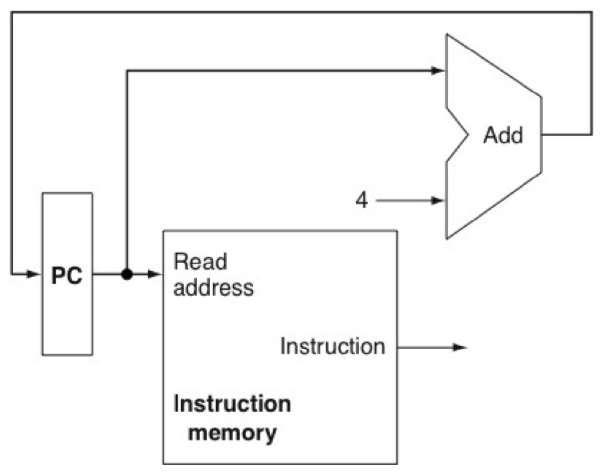
\includegraphics[width=60mm]{img/InstructionFetch.png}
\caption{Instruction Fetch}
\end{figure}

Note this unit also includes an adder to determine what the next instruction address is. Typically this is an increment of 4, but with branches and jumps it will be a different value.


\subsubsection{R-type ALU}

This is how to actually compute things once we have the instruction.

A register file is an array of registers. It has two 5-bit read registers, a 5-bit write register, and a read/write logic signal. Then two outputs that go the ALU unit (which can do addition, shifts, multiplication, or what have you). 


\begin{figure}[ht!]
\centering
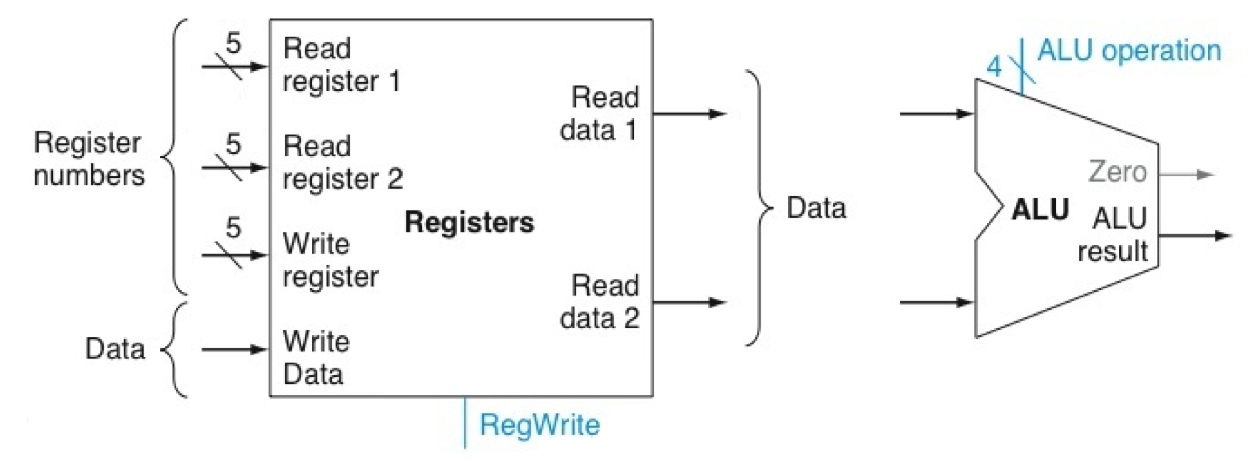
\includegraphics[width=110mm]{img/ALU.png}
\caption{ALU}
\end{figure}


The reason we have 5-bits is because we have 32 registers, so we need 5-bits to identify the correct register. The reason we have two read registers is because some MIPS instructions such as addition or multiplication have two source operands.

\subsubsection{Loads and Stores/Memory}

For now, assume we can use magic memory that can write/read data in one cycle. So we have what we'll call a data-memory unit and a sign-extension unit.

\begin{figure}[ht!]
\centering
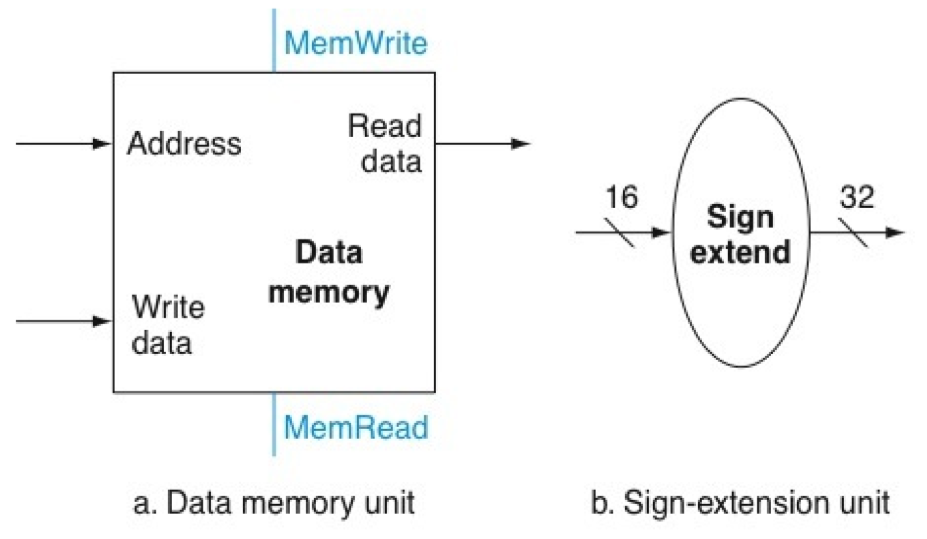
\includegraphics[width=80mm]{img/LoadsAndStores.png}
\caption{Data Memory}
\end{figure}

We have a sign-extension unit because if you read data from memory, some instructions will read 32-bits (word), 64-bits (double word), and some will read a byte. Let's say you're reading an 8-bit negative value \texttt{11111111} and you store it in a 64-bit register, then you'll get the value \texttt{0000000...11111111}, which isn't negative. So you need to run it through the sign extension unit to pad the beginning with 1s.

\subsubsection{Conditional Branches}

This is how we control the flow of a program, so not all instructions are executed in a sequence. Branches allow us to implement conditions and loops. For instance, branch if equal to zero, or branch if these two registers are not equal.

Conditional branches depend on what is coming out of the registers. In order to do this we need to be able to read our two registers and feed them to the ALU for our comparison -- often a subtraction until the result is zero.


\begin{figure}[ht!]
\centering
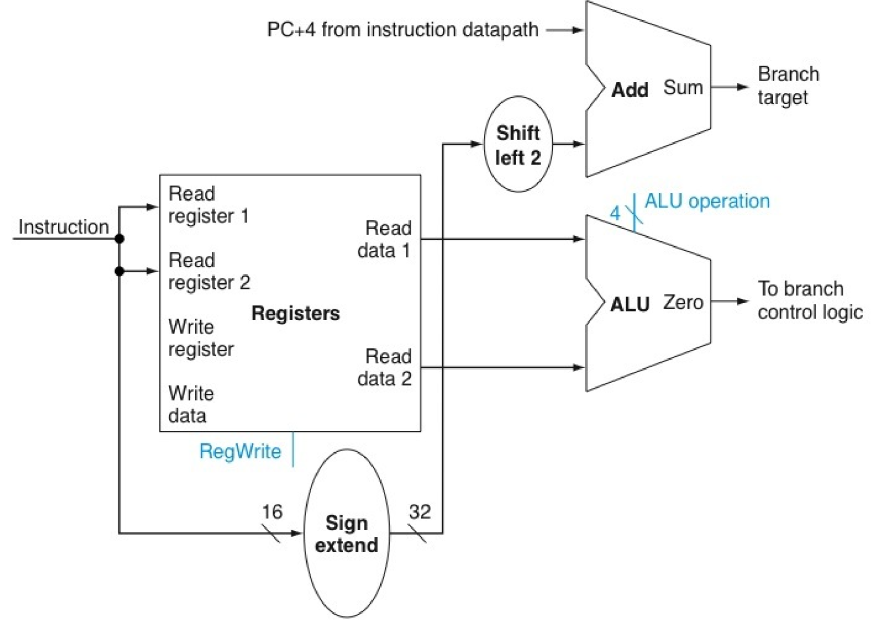
\includegraphics[width=100mm]{img/Branch.png}
\caption{Conditional Branches}
\end{figure}

We also need to figure out the next instruction to be taken. If the branch is to be taken, we need to take the next instruction and add the branch offset, which is relative to the PC.

The reason for the sign extend is so that we can branch both forward and backward, using the sign-extend to allow us to add a negative offset. We shift the instruction left by two because the lower two bits of the instruction address are always zero.

\subsection{Putting it all Together}

\subsubsection{Combining the ALU and the Load/Store}

One of the operations could be coming directly from the memory

\begin{figure}[ht!]
\centering
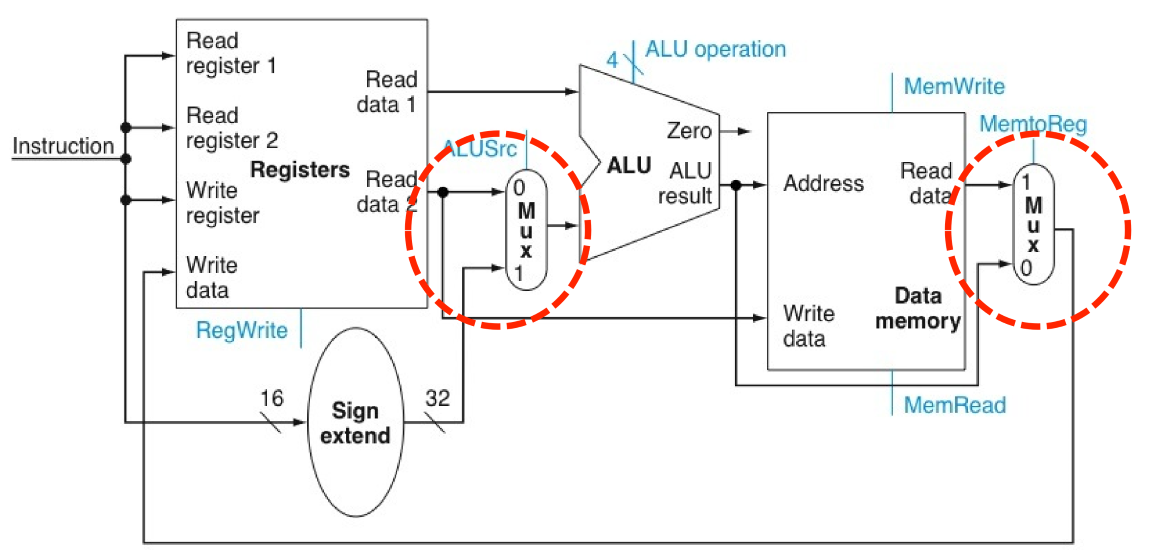
\includegraphics[width=120mm]{img/ALUandLoadStore.png}
\caption{ALU and Load/Store}
\end{figure}

Recall that sometimes load instructions use displacement like \texttt{LD R1, R2(R9)}. In order to pass the value in R2 from the instruction, we need the path with the sign extend that goes around the bottom to the internal mux. Again, this line has the sign-extend so it can pass both negative and positive values.

We also need the mux to decide whether or not to read or store the data. So the mux must decide whether the data is coming from memory or whether it is coming from the ALU operation.

\subsubsection{Combining with Branch/Jumps}

Now we also need the adder to increment the PC. We need the ALU that calculates whether to branch. And we need the mux to determine whether the next PC value is coming from the adder or coming from the conditional of the ALU. 

\begin{figure}[ht!]
\centering
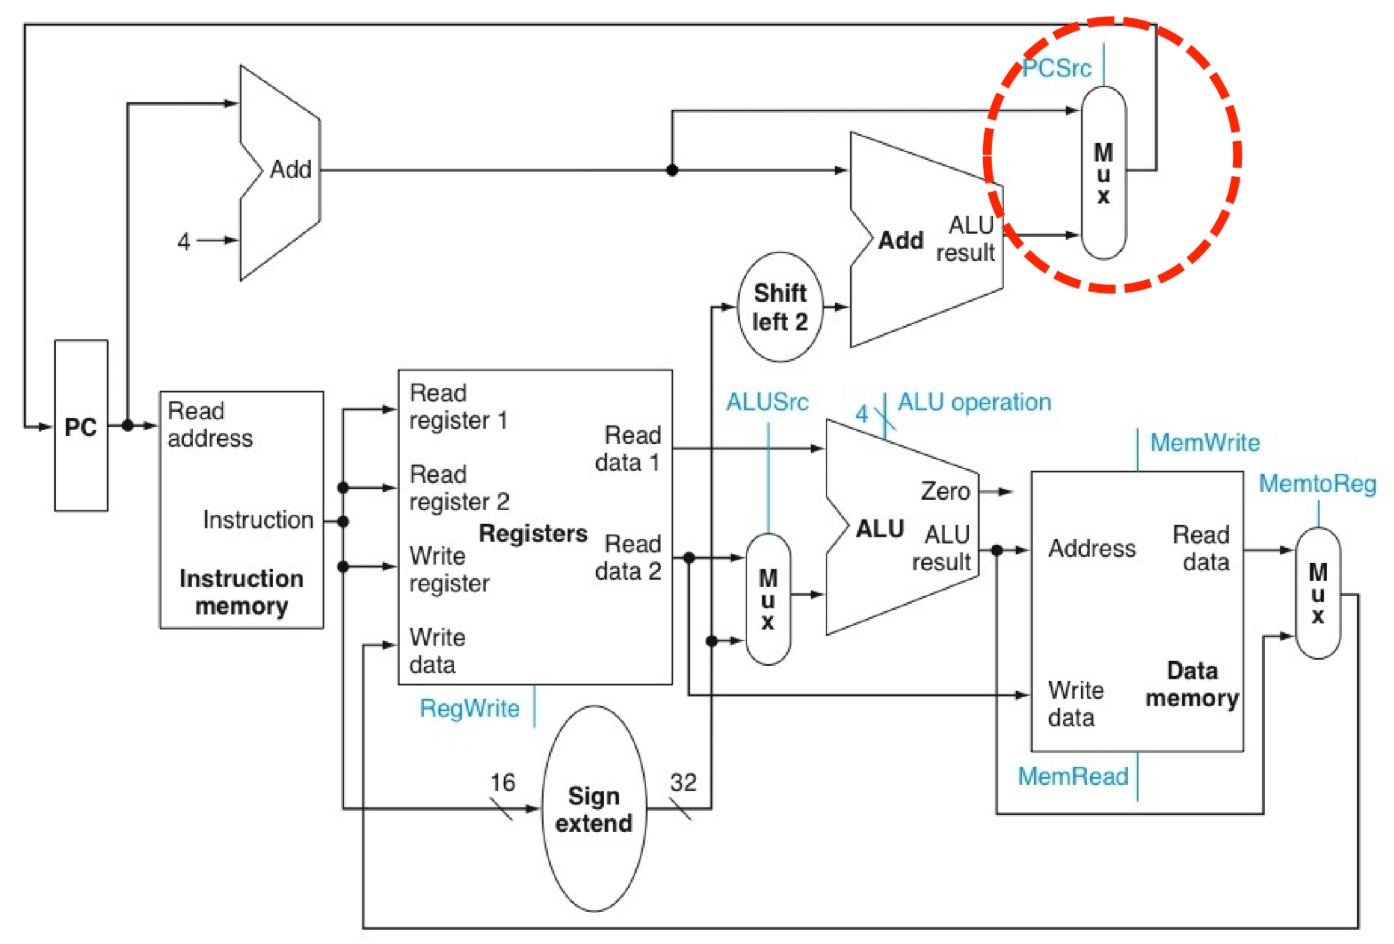
\includegraphics[width=120mm]{img/WithBranchJumps.png}
\caption{ALU and Load/Store}
\end{figure}

\subsubsection{A Full Single-Cycle MIPS64}

Here the ALU operation is coming from the decoded instruction. The control units for the muxes are also coming from the decoded instructions. 

If the instruction is a load instruction, the mux on the far right tells the CPU to store the value from the memory, if it's not, the CPU will store the value from the ALU operations.

If the instruction is to branch and the result of the operation is to branch, then the PC will be incremented by the result of the ALU operation on top, not the adder, and so on.

\begin{figure}[ht!]
\centering
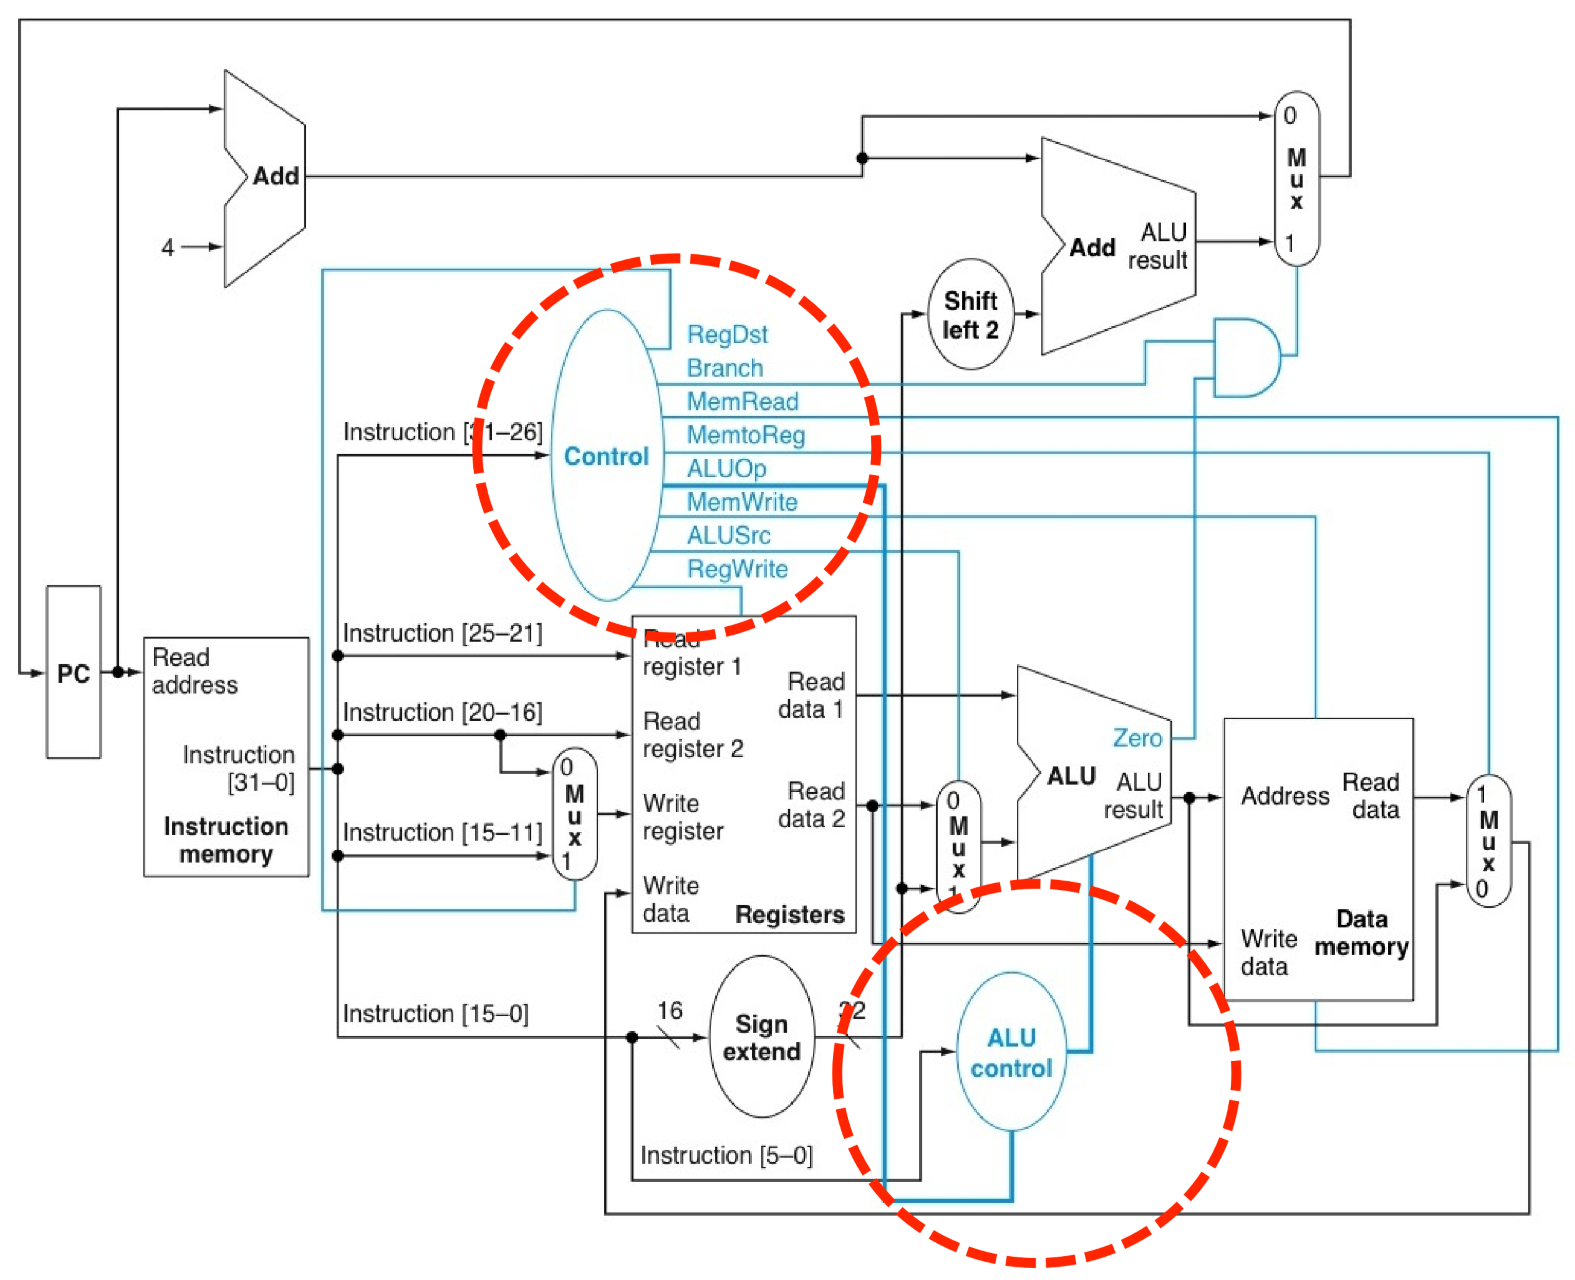
\includegraphics[width=120mm]{img/SingleCycleMIPS.png}
\caption{Single-Cycle MIPS64}
\end{figure}

\subsection{Actual Pipelining}

Now we can make the single-cycle MIPS perform well by taking advantage of pipelining.  The main benefit of MIPS being a register-register architecture is that we can take full advantage of pipelining. 

\begin{figure}[ht!]
\centering
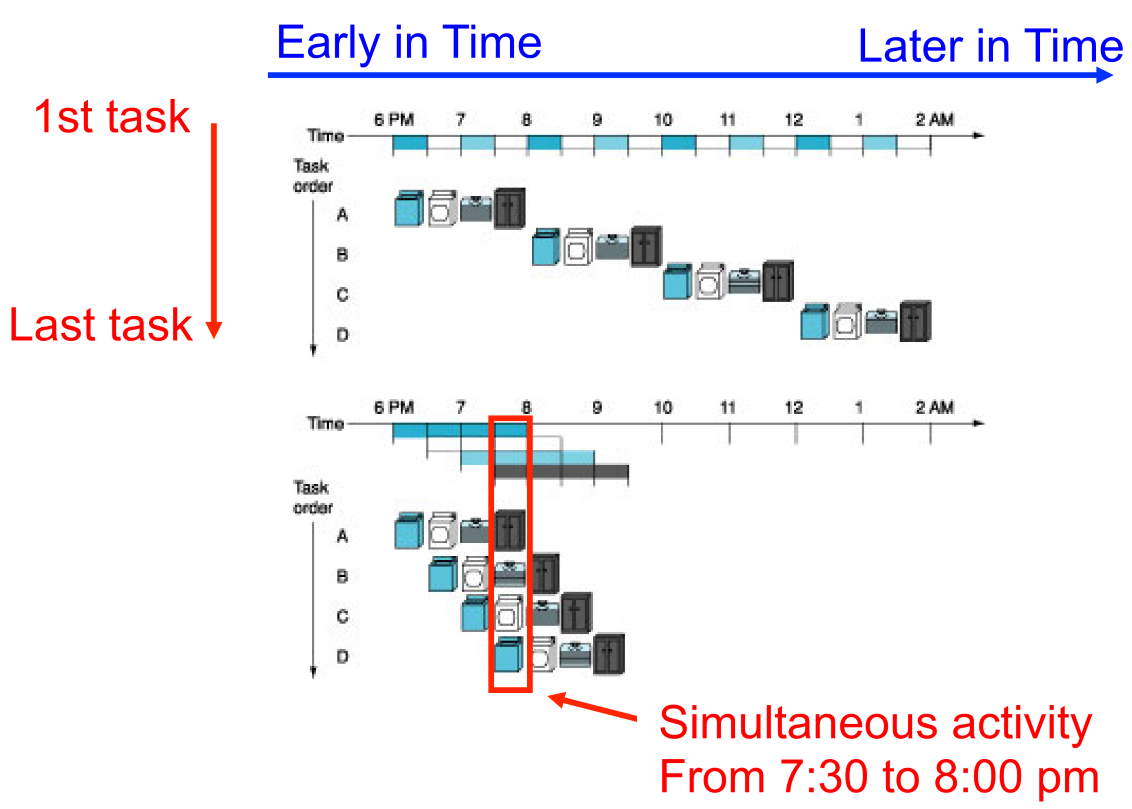
\includegraphics[width=90mm]{img/Pipelining.png}
\caption{Pipelining Analogy}
\end{figure}

In the analog in Figure 17, the washer/dryer/ironing board/closet are "function units". If you At any given point, you can be doing different operations relating to different instructions (loads of laundry) simultaneously. 

The main benefit of the assembly line wasn't only specialization, it was that since there were multiple cars being produced at once, different workers could be working on different elements of different cars simultaneously. 

Pipelining works best when tasks are broken up into specific sequential operations, which is why MIPS instructions are broken up into such rigid steps of instruction processing. 

If there are four steps in the process, the pipelining can be four times as fast as a sequential process. To pipelining to need some sort of state, like latches, to hold the value between operations.

\subsubsection{Example -- Floating Point Multiplier}

In the case of an unpipelined multiplier, each result is completed before the next multiplication is started. But that means that after, for instance, the normalizing step is completed, the normalizing unit is doing nothing and just waiting for its next input.

\begin{figure}[ht!]
\centering
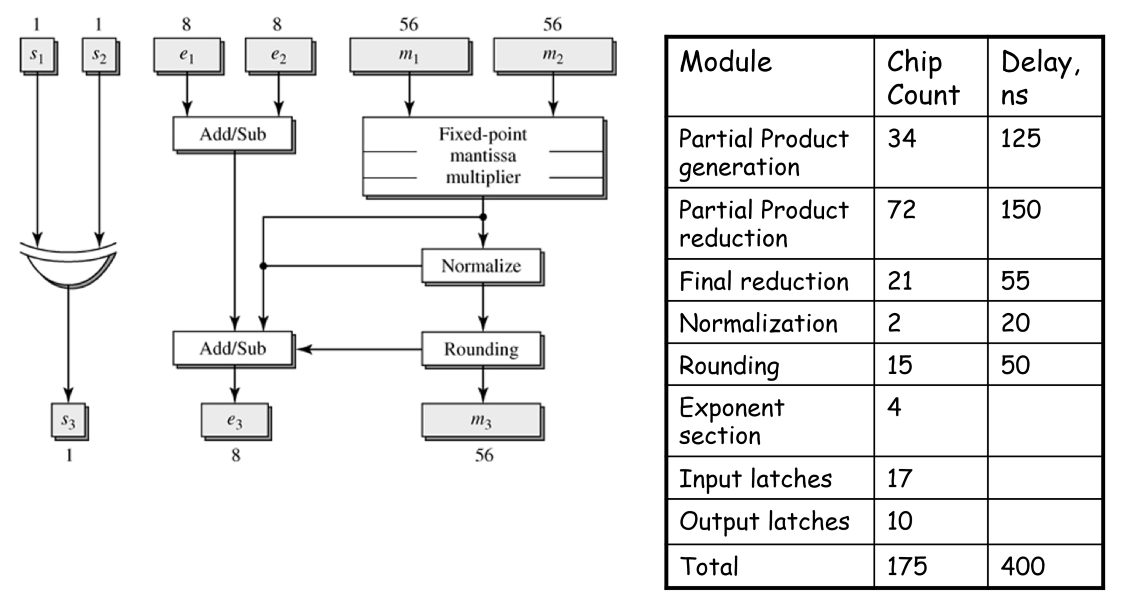
\includegraphics[width=100mm]{img/FloatingPoint.png}
\caption{Unpipelined Floating-Point Multiplier}
\end{figure}

With the pipelined version, latches are introduced in between each step. That way when the normalizing step is completed, it can immediately begin normalizing for the next operation. 

Note that there are multiple latches on the same wire in the pipelined version. This is because the exponent and the mantissa need to arrive at the output at the same time.

The other thing you want with pipelining is for the stages to have similarly timed latencies so that one operation isn't waiting for another to complete before the next operation can begin. This is why the third stage has three units, all of whom add up to a similar latency to the one block in the previous two stages. 

\begin{figure}[ht!]
\centering
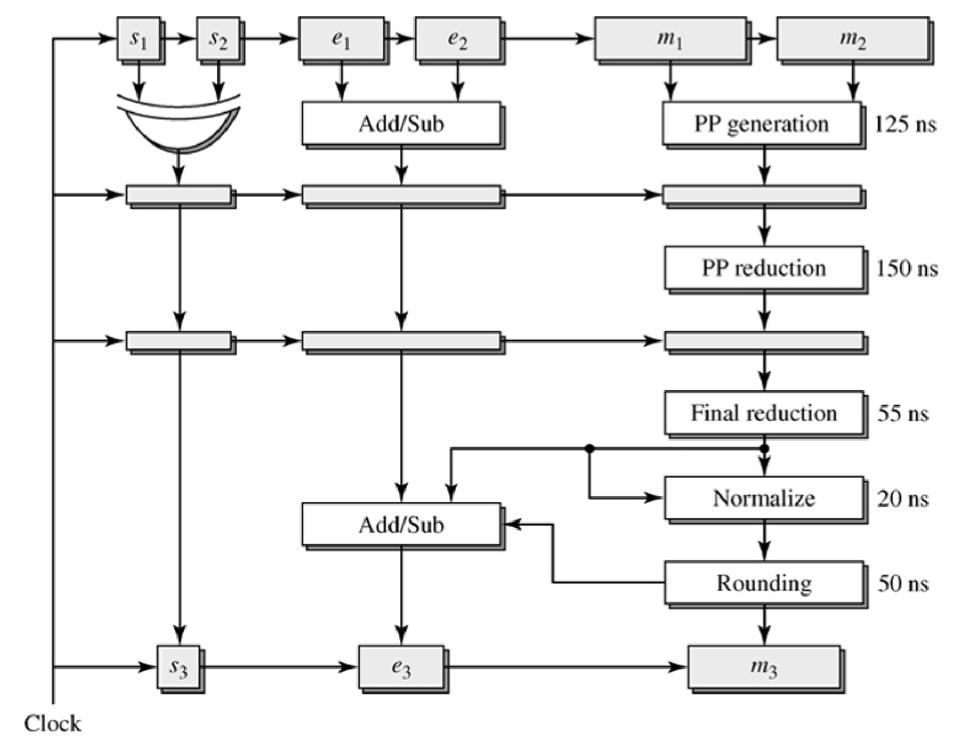
\includegraphics[width=80mm]{img/FloatingPointPipe.png}
\caption{Pipelined Floating-Point Multiplier}
\end{figure}

This pipelining comes at a cost. Individual instructions can have more latency, because of the setup times and clk-to-output. You also need more storage to hold the intermediate values, and it costs more to implement these extra ICs.

Note that although you're breaking up this operation into three stages, you're not getting $3\times$ the performance. In reality it's about $\frac{400ns}{172ns} = 2.3\times$ the performance. This is because not all stages have the exact same delay, so some stages will take longer and these will hold back the other stages. And as discussed, there is a little bit of overhead due to latch latency. 

However, you cannot always use a pipelined circuit for any sequence of floating point operations. If you are doing operations such as $y=ab+c$, you need to determine the final value of $ab$ before you can add $c$. 

\subsection{Desirable Traits of Pipelining}

\begin{enumerate}

\item \textbf{Uniform subcomputations} -- each stage has the same delay, so slower stages aren't holding back faster stages

\item \textbf{Identical computations} -- each computation uses the same number of stages, so that in each cycle each stage is doing some work

\item \textbf{Independent computations} -- if you have data-dependencies (for instance because of BEDMAS), it might limit your ability to take advantage of pipelining

\end{enumerate}

The first RISC processors were about 100k gates. The first pipelined processor was about 30k gates. This was back when ISA mattered more than it does now.

\subsection{Pipelining MIPS}

Like we said before, pipelining requires instructions to be broken into roughly equal subcomputations. Luckily, the MIPS ISA can be broken up into the five logical stages 

\begin{enumerate}

\item \textbf{F} Instruction Fetch -- indexes the instruction memory
\item \textbf{D} Instruction Decode -- reads the operands from the register file
\item \textbf{X} Execute -- actually computes the result
\item \textbf{M} Memory Access -- where we read/write from memory
\item \textbf{W} Write Back -- decide to write back from memory or from the ALU

\end{enumerate}

\begin{figure}[ht!]
\centering
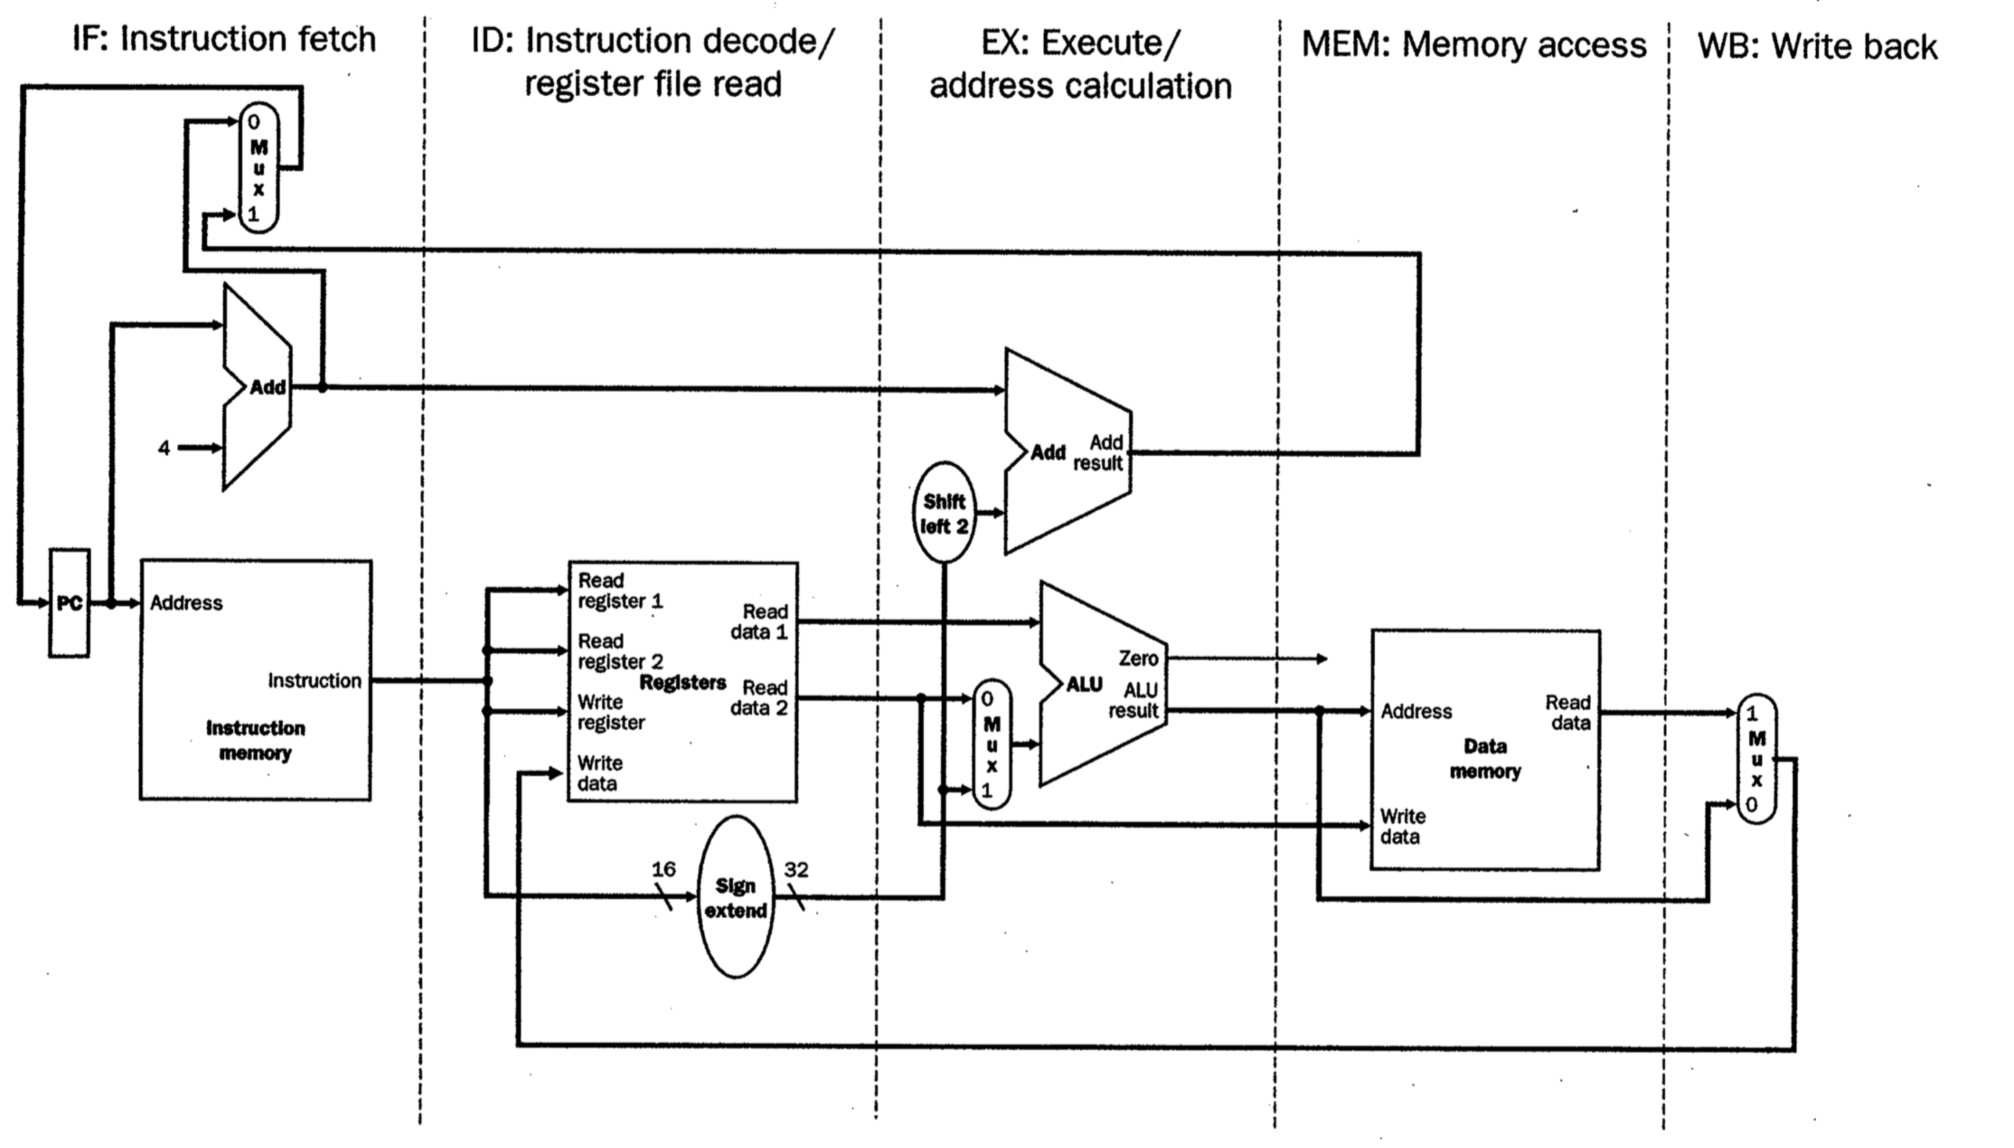
\includegraphics[width=120mm]{img/PipeliningMIPS.png}
\caption{Pipelining MIPS}
\end{figure}

The nice thing about stretching it out like this is we can put in registers in between each step to held the temporary values. However, note that these registers are not visible or accessible to the programmer. This is all abstracted away. 


\begin{figure}[ht!]
\centering
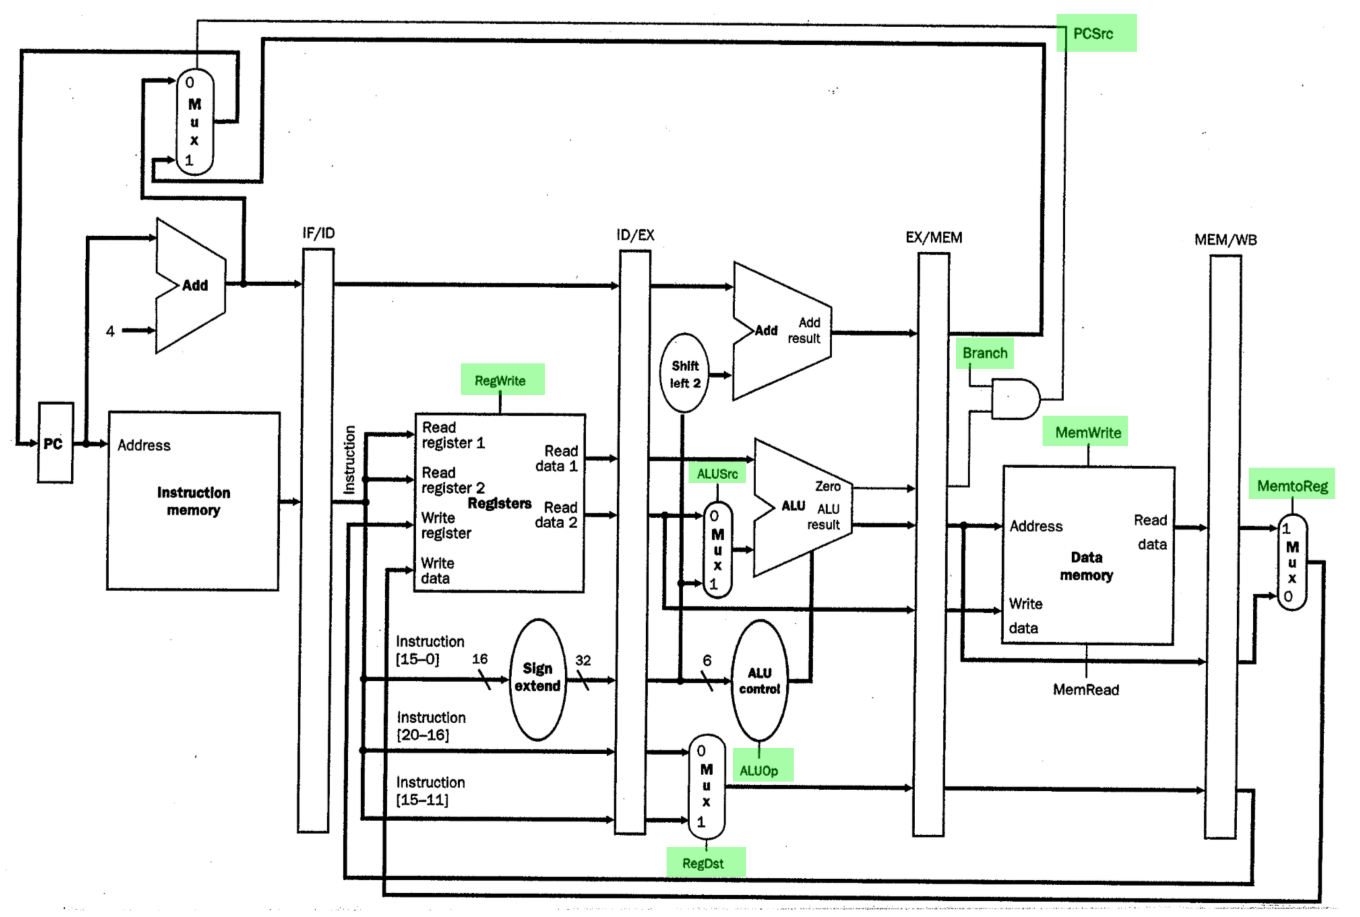
\includegraphics[width=110mm]{img/PipeliningMIPSRegs.png}
\caption{Pipelining MIPS with Registers and Control Signals}
\end{figure}

Recall the desirable traits of pipelining were that there were

\begin{enumerate}
\item Uniform subcomputations -- in MIPS, these stages are pretty well balanced even though there is some disparity between processor and memory

\item Identical computations -- that is, that each computation uses roughly the same number of stages. It's mostly true, although some instructions like jumps or ALU operations don't use all, they use most

\item Independent computations -- when you have one instruction that depends on another, since we're using a register-register ISA, these dependencies are easier to identify

\end{enumerate}

RISC  architectures were designed in such a way to simplify the hardware and take full advantage of pipelining.

\subsubsection{Hazards}

A way to portray pipelined instructions is as demonstrated in Table 5. This breaks up the different stages of an instruction into its five components IF, ID, EX, MEM, WB and sees how they layer, and what stages of what instructions are being executed in parallel. 

It is often very important to see what is happening at the same time. This more easily allows you identify hazards. A common hazards is the RAW, which is the Read-before-write. For instance, consider the first instruction in Table 5. This writes the sum of R2 and R3 to R1. 

\begin{table}[H]
\small
\centering
\caption{MIPS Pipelining Hazards}
\begin{tabular}{lccccccccc}
\toprule
\textbf{Clock cycle} 		& 1 	& 2 	& 3 	& 4 	& 5 	& 6 	& 7 	& 8 	& 9   	\\ 
\midrule
\texttt{DADD R1, R2, R3} 	& IF 	& ID 	& EX 	& MEM 	& WB  	& 		& 		& 		&  		\\
\texttt{DSUB R4, R1, R5} 	&		& IF 	& ID 	& EX 	& MEM 	& WB  	& 		& 		& 		\\
\texttt{AND  R6, R1, R7} 	&		&		& IF 	& ID 	& EX 	& MEM 	& WB  	& 		& 	  	\\
\texttt{OR   R8, R1, R9} 	&		&		&		& IF 	& ID 	& EX 	& MEM 	& WB  	&  	  	\\
\texttt{XOR  R10, R1, R11} 	&		&		&		&		& IF 	& ID 	& EX 	& MEM 	& WB  	\\
\bottomrule
\end{tabular}
\end{table}

However, this instruction is not completed until clock-cycle 5, so until clock-cycle 5, R1 is not updated. Yet if this code was pipelined, the second and third instructions would already start doing operations using the not-yet-updated value in R1. You will have the value of R1 by the beginning of the WB stage in cycle 4.


Hazards are when you might need a piece of data from one operation in a following operation, but that value may not yet have been computed. There are multiple types of hazards

\begin{enumerate}

\item \textbf{Structural hazards} -- these are caused by resource conflicts, where two or more instructions may want to use the same hardware at the same time. 

Structural hazards can always been resolved by simple stall, which means to simply wait a few clock cycles until the previous instruction is completed using the resource. Stalls can reduce performance a little bit.

Alternatively, you can add extra hardware. You can add duplicate adders, you can add duplicate registers, etc. 


\item \textbf{Data hazards} -- This is the RAW case mentioned above, where the following instruction relies on information determined/saved by a previous incomplete instruction. It's impossible to send data "back in time", so to speak.

You may be able to forward data to parallel stages however. This requires hardware support, even if the instruction started in a previous stage but didn't require the data until that stage. 

\item \textbf{Control hazards} -- A branch is conditional, so it may or may not change the PC. But by the time you decide what the value of PC should be, you have already begun processing the next instruction. Typically, by the EX or the ID stage, you will know what the branch will be. 

You can either stall until the result of the branch instruction is determined, or you can guess. The processor can guess that the branch is not going to be taken, and start to execute the next instruction. Then if the branch turns out it isn't going to be taken, it can cancel the instruction. 

\end{enumerate}

\subsubsection*{Example}

Let's say 40\% of instructions are data memory references. Without structural hazards, CPI=1. Which processor is faster, a processor with structural hazard that has a clock rate that is 1.05 times faster, or the processor without structural hazard?

---

This means 40\% of the time, the processor with the hazard will have to stall for the load for one extra cycle. So the cycles per instruction will be 1+40\%

$Execution\ time_{with} = (IC)(CPI)(Cycle\ time) = (IC)(1 + 0.40)(Cycle\ time)$

$Execution\ time_{without} = (IC)(1)(1.05 \times Cycle\ time)$

$Speedup_{without} = \dfrac{ExT_{with}}{ExT_{without}} = \dfrac{1+0.40}{1.05} = \textbf{1.33}$

---

\subsection{Dependencies}

A dependency is when two instructions executed in a different order could yield a different result. This limits how much we can reorder and parallelize our instructions.

Data dependencies are a property of the program itself, not the hardware. It doesn't matter if you were running single-cycle MIPS, 5-cycle MIPS, or out of order execution, you'll still get data dependencies. 

Hazards however, are a property of the hardware. This is when an execution of an instruction can violate a data dependency. 

\subsubsection{True Dependency}

A true dependency is the classic data dependency, it is when a value is communicated across instructions. These cause a RAW hazard.

\begin{Verbatim}
DADD R1, R2, R3
DSUB R4, R1, R3
\end{Verbatim}

Here, the value stored in \texttt{R1} by the \texttt{DADD} operation is communicated to the \texttt{DSUB} operation. If the hardware can perform the read of \texttt{R1} in the \texttt{DSUB} instruction before the write of the previous instruction, you will get a RAW hazard.

\subsubsection{Name Dependency}

A name dependency is when two instructions use the same piece of hardware (usually register or memory location), but no data passes between them. That is, the dependency is on the data address (name), not the value. These cause a WAR hazard.

\begin{Verbatim}
DSUB R4, R1, R3
DADD R1, R2, R3
XOR  R6, R1, R7
\end{Verbatim}

For instance in the above instructions, \texttt{R1} is used for some initial operation, then reused for some second operation. This is an "anti-depedency" because it's not a true dependency, instead it results from the reuse of the R1 register. 

The first instruction must finish reading R1 before the second instruction writes to R1. If the first and second operations were reversed, this would change the result of the third instruction.

Because of this, is still a depedency because if the instructions are reordered there is a different result. 

\subsubsection{Output Dependency}

Output dependencies are when two instructions write to the same register, these cause a WAW hazard.

\begin{Verbatim}
DSUB R1, R4, R3
DADD R1, R2, R3
XOR  R6, R1, R7
\end{Verbatim}

Here, if the first instruction takes longer than the second instruction, it will leave the wrong value in \texttt{R1} which will result in the wrong value being used in the third instruction.

This also results form the reuse of the register, but is a dependency because again, reordering the instructions will yield a different result.

\subsubsection*{Example}

List the true, anti, and output dependencies in this code.

\begin{Verbatim}
I:  L.D     F6, 34(R2)
J:  L.D     F2, 45(R3)
K:  MUL.D   F0, F2, F4
L:  SUB.D   F8, F6, F2
M:  DIV.D   F9, F0, F6
N:  ADD.D   F6, F8, F2
\end{Verbatim}

---

\noindent True dependencies -- RAW hazards 

\begin{itemize}

\item \texttt{F2} between J and K, J and M, J and N
\item \texttt{F0} between K and M
\item \texttt{F6} between I and L, I and M
\item \texttt{F8} between L and N
\end{itemize}

\noindent Anti dependencies -- WAR hazards

\begin{itemize}

\item \texttt{F6} between M and N  
\end{itemize}

\noindent Output dependencies -- RAR hazards 

\begin{itemize}
\item \texttt{F6} between I and N, I and L
\end{itemize}

\subsection{Multicycle Operations}

Some operations have different numbers of cycles to complete, for instance most floating point operations take many more cycles than integer operations, and division takes much longer than addition. 


\begin{figure}[ht!]
\centering
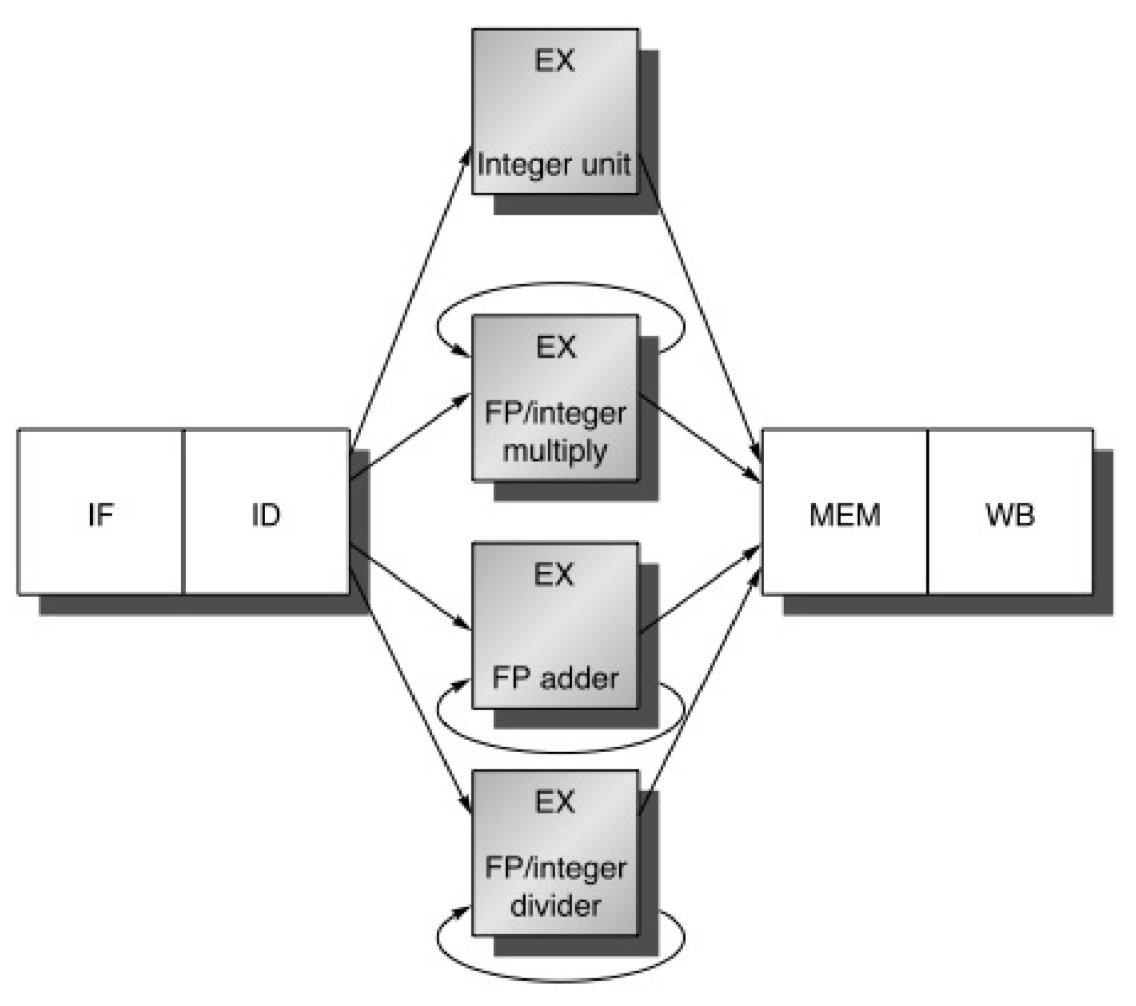
\includegraphics[width=70mm]{img/MulticycleOperations.png}
\caption{Multicycle Operations}
\end{figure}

RAW hazards are still an issue because by the time we have written our value from a long floating point operation, we could have already read the stale value for a short subsequent operation.

WAW hazards are now an issue. Assume it takes five cycles to do floating point addition instruction, then you do an integer addition instruction afterward which takes one cycle afterward. The integer operation will be completed first and write that value, then the floating point operation will complete and overwrite the register with the wrong value.

WAR hazards are no longer an issue however. (???)

 \subsection{Pipelined Function Units}

Now we can get more instructions through simultaneously if are there are no dependencies stopping you. We still will have structural hazards because many instructions will want to be using the memory and write-back at the same time.

We will also get WAW hazards because the writing back will happen in an order that is different from the instruction order because different instructions have different latencies.

\begin{figure}[ht!]
\centering
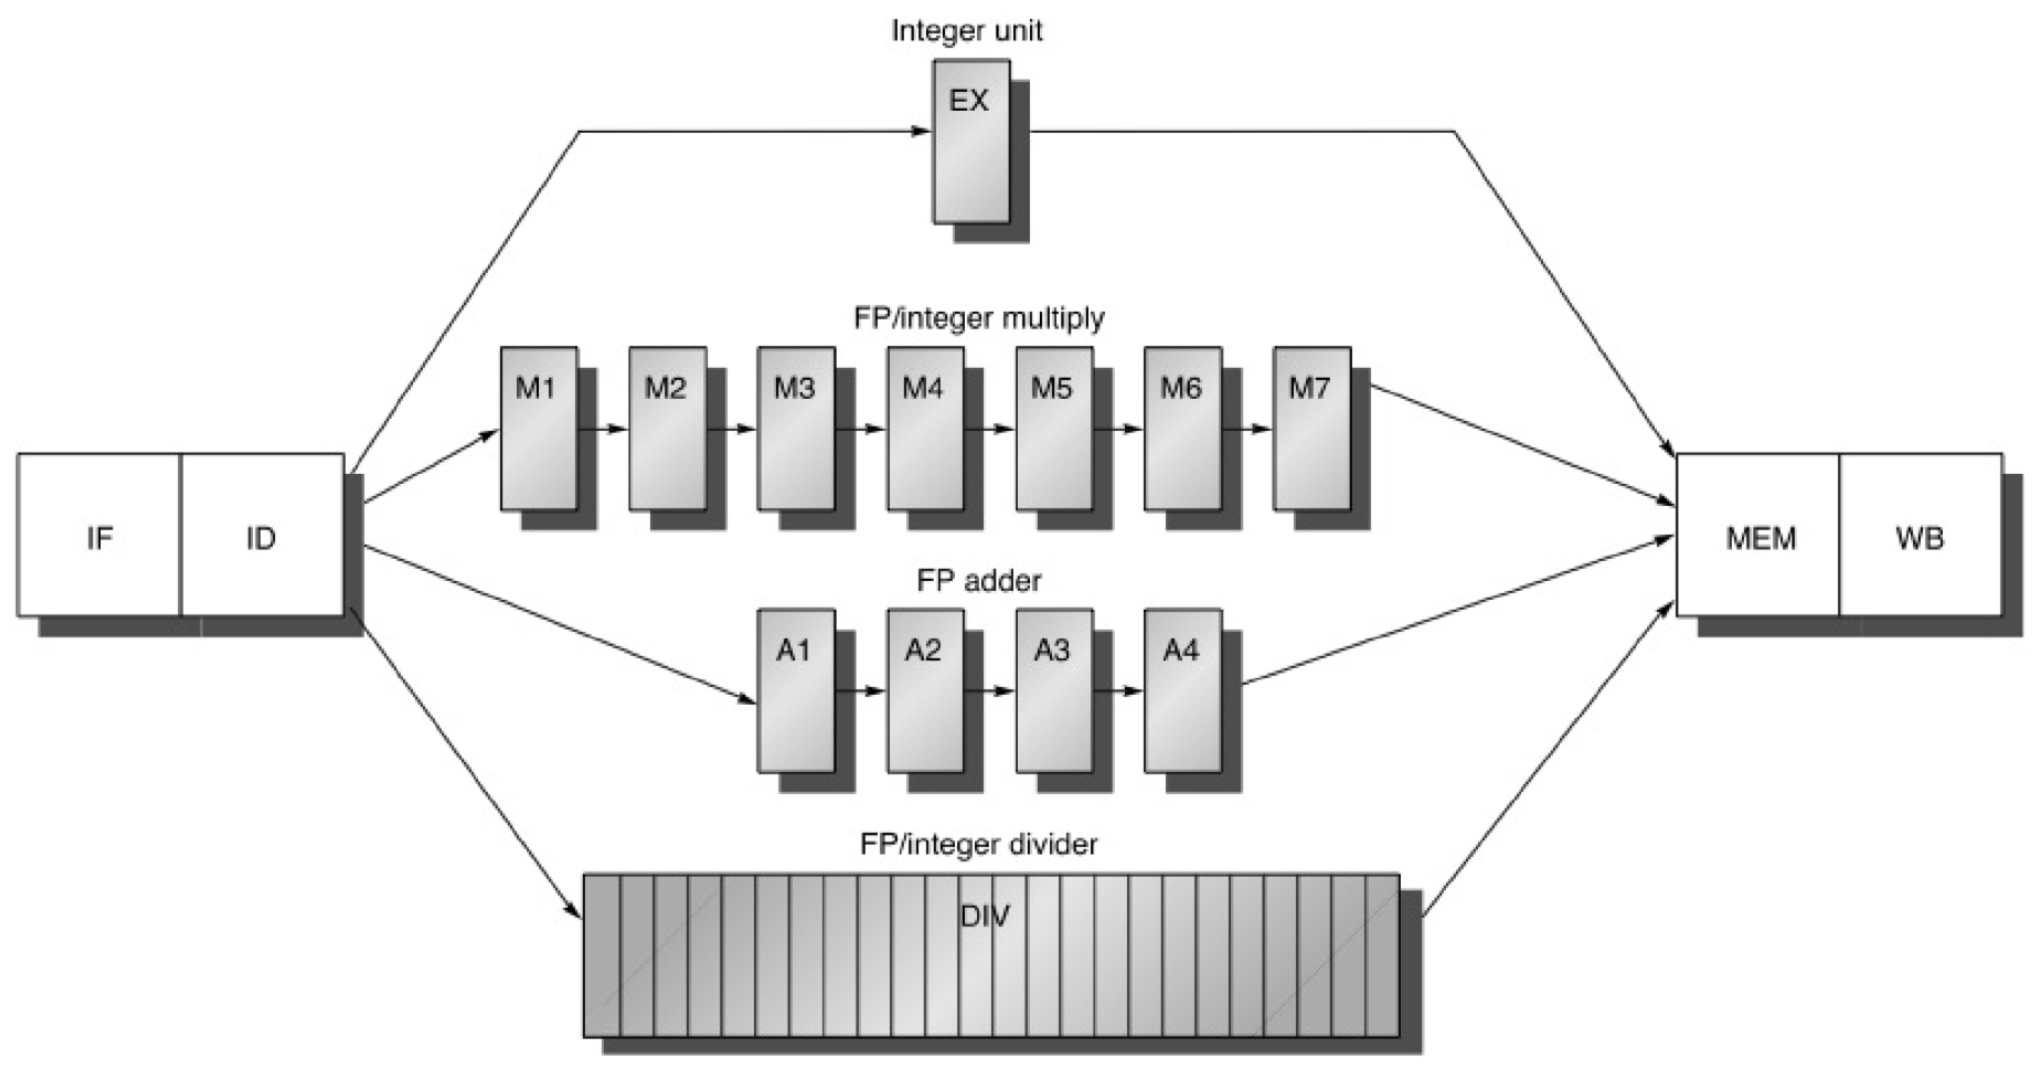
\includegraphics[width=120mm]{img/PipelinedFU.png}
\caption{Multicycle Operations}
\end{figure}

\subsubsection{In-order Scoreboard for Multicycle Pipelines}

In the decode stage, we look at the destination register and set the bit related to that register. That instruction is reserving that register until it has completed writing to it.

This array of bits that signal in-use registers is called the scoreboard. If the bit is not set, the register has valid data, and if the bit it set, it has stale data. So we can track which registers are going to be overwritten. 

If any other instruction will read or write from a register with a set bit in the scoreboard, we will stall until the instruction that has reserved the register is completed and clears the bit. This allows us to issue commands in order, but execute them out of order.

\paragraph{Algorithm}

When issuing commands/reading operands (in order):

\begin{enumerate}

\item If either source register is set, then there is a RAW hazard, so stall.

\item If the destination register is set, then there is a WAW hazard, so stall.

\item Otherwise, dispatch the instruction to the functional unit and set the destination register bit. 

\end{enumerate}

\noindent When completing commands (out of order):

\begin{enumerate}
\item Update the destination register and clear the scoreboard bit.

\end{enumerate}


If you know how long the operation is you know how long to stall for, so you can schedule instructions to start at the end. 

If you know how long the instructions are, then let's say you have a long floating point division operation, you could fit in a parallel non-dependent short instruction into the time where it's stalling. This allows you to take even more full advantage of your hardware.

This is implemented with a Shift Register. (???)



\section{Out-of-Order Execution}

Out-of-Order (OoO) execution is important because some instructions do not have dependencies on the previous instructions. If these instructions are executed in order, then it's possible while one that requires a dependency is stalling, the following instructions are being stalled unnecessarily. 

Consider the following example
\begin{Verbatim}
i1:  DIV.D  F0, ...
i2:  MUL.D  F2, ...
i3:  ADD.D  F14, F2, F0
i4:  DADD   R4, R5, R6
i6:  ADD.D  F8, F10, F12
\end{Verbatim}

Instruction i3 is dependent on i1 and i2, but i4 and i5 have no dependencies. So while i3 is stalling for i1 and i2 to complete, which takes many cycles for floating-point operations, i4 and i5 could have been executed in parallel. This is called head of the line blocking.

\begin{figure}[ht!]
\centering
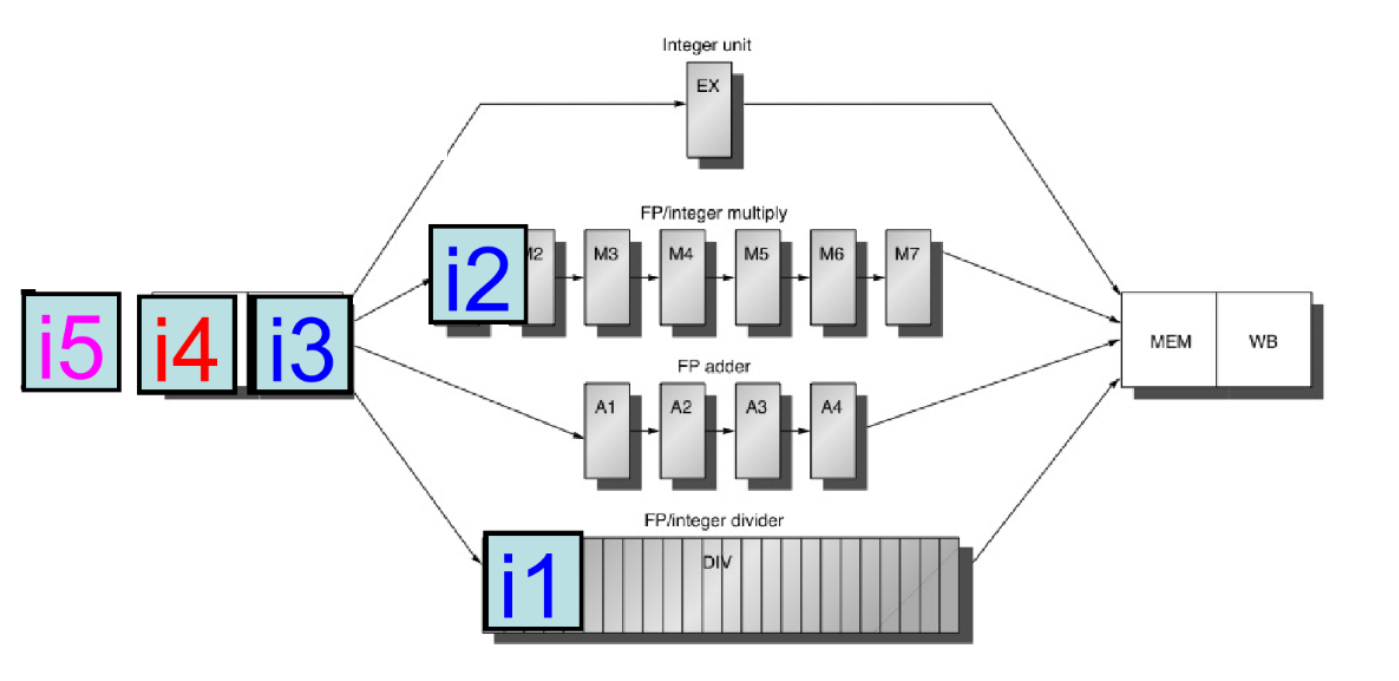
\includegraphics[width=80mm]{img/HOLB.png}
\caption{Head of the line blocking}
\end{figure}

To take advantage of this, it requires some additional hardware. 


\subsection{Decode Instruction}

In the decode stage we can determine the destination register and mark it as "stale", meaning waiting to be read to. This tells the other instructions that if they are going to write to that register, they will be overwritten and should stall until it is no  longer stale. This must be done in order.

We also should read the operands needed for computation (???),  we can do this out of order so long as we wait until the operands are no longer stale.

Now we split the decode into two steps:

\begin{enumerate}
\item \textbf{Issue} -- Decode instruction + check for structural hazard check

\item \textbf{Read operands} -- Wait until there are no data hazards
\end{enumerate}

\subsection{Scoreboards}

A scoreboard allows us to keep track of what registers are and are being used to help us with our OoO executions. 

\subsubsection{Scoreboard Algorithm}

\begin{enumerate}
\item \textbf{Issue} -- Check if functional unit (FU) is available and check that no other instructions have the same destination register (WAW hazard). If so, stall to resolve WAW hazards.

\item \textbf{Read operands} -- Wait until source operands are available if currently in use (in flight), and then read them and start execution. This resolves RAW hazards dynamically.

\item \textbf{Execution} -- Notify the scoreboard when the functional unit is no longer using the operand registers.

\item \textbf{Write Results} -- Once executed, before writing our result to the destination register, we must check for WAR hazards. If someone is still waiting to read the operands we're about to write, they'll read the new value instead of the one they were meant to read. If no WAR hazard, write the result.

\end{enumerate}

\subsubsection{Scoreboard Components}


\begin{tabular}{ll}
\textbf{Flag} & \textbf{Job} \\
\toprule
Busy flag & Indicates unit is busy \\
Op & Operation to perform in unit \\
$F_i$ & Destination register number \\
$F_j,\ F_k$ & Source register numbers \\
$Q_j,\ Q_k$ & Function units producing $F_j,\ F_k$ (???) \\
$R_j,\ R_k$ & Flags indicating when $F_j,\ F_k$ are ready \\

\bottomrule
\end{tabular}


\section{Register-Renaming}

Recall our hazards and how we deal with them so far:

\begin{enumerate}

\item \textbf{Pipelining} causes overlapping instructions, so you can read a register value before it is written to -- \textbf{RAW hazards}. These are fixed by stalling and forwarding.

\item \textbf{Concurrent execution} in different functional units, means that FUs with different latencies will complete out-of-order, so a register can be overwritten by a previous instruction -- \textbf{WAW hazards}. These are fixed by tracking in use registers with a scoreboard and stalling.

\item Scoreboard scheme allows us to \textbf{read operands out of order}. But reading operands out-of-order means that an instruction can overwrite a value in a register before it is read by a previous instruction, so the previous instruction will read the wrong value -- \textbf{WAR hazards}. These are resolved by stalling if the destination register is still pending.

\end{enumerate}

Recall WAW and WAR hazards are the product of reusing registers, they are name dependencies. This means they would be eliminated if we had an infinite supply of names. 

Observe the following code. We can rename each destination register with a fresh tag name. By doing this we eliminate all WAW and WAR hazards.

\begin{verbatim}
LD      R1, 0(R2)     ->    LD      T1, 0(R1)      
DADD    R3, R1, R3    ->    DADD    T2, T1, R3
DADDUI  R3, R2, #8    ->    DADDUI  T3, R2, #8      
LD      R1, 0(R2)     ->    LD      T4, 0(T3)
\end{verbatim}

\subsection{Tomasulo algorithm}

Registers in instructions are renamed to tags. Each destination register gets a fresh tag, and the tag is mapped to the register in the register alias table (RAT). Source registers get corresponding tags from the RAT. 

This way we track data dependencies directly and there are no WAW or WAR hazards, only true dependencies in RAW hazards. 

Reservation stations (RSs) are put in from of each functional unit. This way we can buffer instructions that are waiting for operands. 

When the results are computed, the result and the tag of the source is broadcast on the common data bus (CDB). As RSs listen to the CDB for tags they want values for.

\begin{enumerate}
\item \textbf{Issue} -- If we have an available RS, allocate RS entry. Lookup source operand registers in the register file and get either the values or the tags. Rename the destination register to the allocated RS entry. 

\item \textbf{Execute} -- Listen to the CDB for operands tags that aren't ready yet, and execute when they're all ready. 

\item \textbf{Write result} -- Broadcast the destination tag and the result on the CDB, interested reservation tags will use this. Mark reservation station available.
\end{enumerate}

This eliminates two of our three hazards, but it is complicated to implement, and it requires a lot of hardware which has high capacitance and limits speed. Also, only one FU can complete per cycle because only one thing can be broadcast on the CDB per cycle. You could implement multiple CDBs, but now we're getting even more complicated. 

\section{In-order commit and multiple issue}

Now we're going to have to deal with exceptions, and speculative executions, implementing a reorder buffer (to ensure in-order commit), and issuing multiple instructions simultaneously (superscalar). 

\subsection{Exceptions}

Exceptions, like interrupts, segmentation faults, divide by zeros, breakpoints, and page faults are detected at execution time. These require transfer of control to another program, but may need to resume the original program as if nothing had happened.

\textbf{Precise exceptions} are supported when the architecture completes all instructions before the exception, and no instructions after the exception have been executed. 

\subsubsection{In-order pipeline}

Upon detection of an exception:

\begin{enumerate}
\item Switch instruction fetch to exception handler

\item Convert instructions in the pipeline after and including the exception instruction to no operations (NOPs or "bubbles")

\item Save the PC of faulting instruction to the EPC register so we can resume later
\end{enumerate}

Make sure you stop precisely at the exception -- don't execute any instructions afterward and finish executing everything before.

\subsubsection{Out-of-order commit}

Precise exceptions are hard with OoO execution because the RF may have values stored in it that have been computed by later instructions. This means we have to save the values before committing them to the RF until we are sure there has been no exception. 

\subsection{Speculative Execution}

Speculative execution is somewhat similar to prices exceptions, because if you choose incorrectly you have to make sure you cancel purge any instructions that have been completed as part of a mispredicted path. 

Statistically, most branches are taken. Think of loops, usually they branch back to the same location, then at the end of the loop continue. All high-performance CPUs are speculative. The compiler can usually product the outcome with about 85\% accuracy, then the hardware can predict it with 95-98\% accuracy. 

Consider the following instructions:

\begin{verbatim}
       DIVD    R3, R1, R2
       BEQZ    R3, Label
       ...
Label: DMUL    R4, R4, R2
\end{verbatim}

Suppose the branch is mispredicted to be taken, then R4 would be modified in the register file, and when we cancelled the instruction we would have lost the correct value of R4. So we cannot let DMUL write to the register file until we know this is the correct branch.

\subsection{Completion and commit}

Here we can see the issue is writing to the RF, not speculating or finishing the computation early. To fix this we can compute the result, but delay writing to the RF until we know the previous instructions weren't speculative and didn't throw exceptions.

To do this, we will split writeback into two stages called completion and commit. Completion means we have computed the result so instructions afterward can read it, but you don't write it to the RF yet. Then you commit once you know you're safe.

\subsubsection{Reorder Buffer (ROB)}

We queue the instructions in the program order (a FIFO) then buffer the computed results in the ROB before we do the RF write. The instruction results can be computed in the wrong order, but the ROB stores them and commits them in the program order.


\begin{figure}[ht!]
\centering
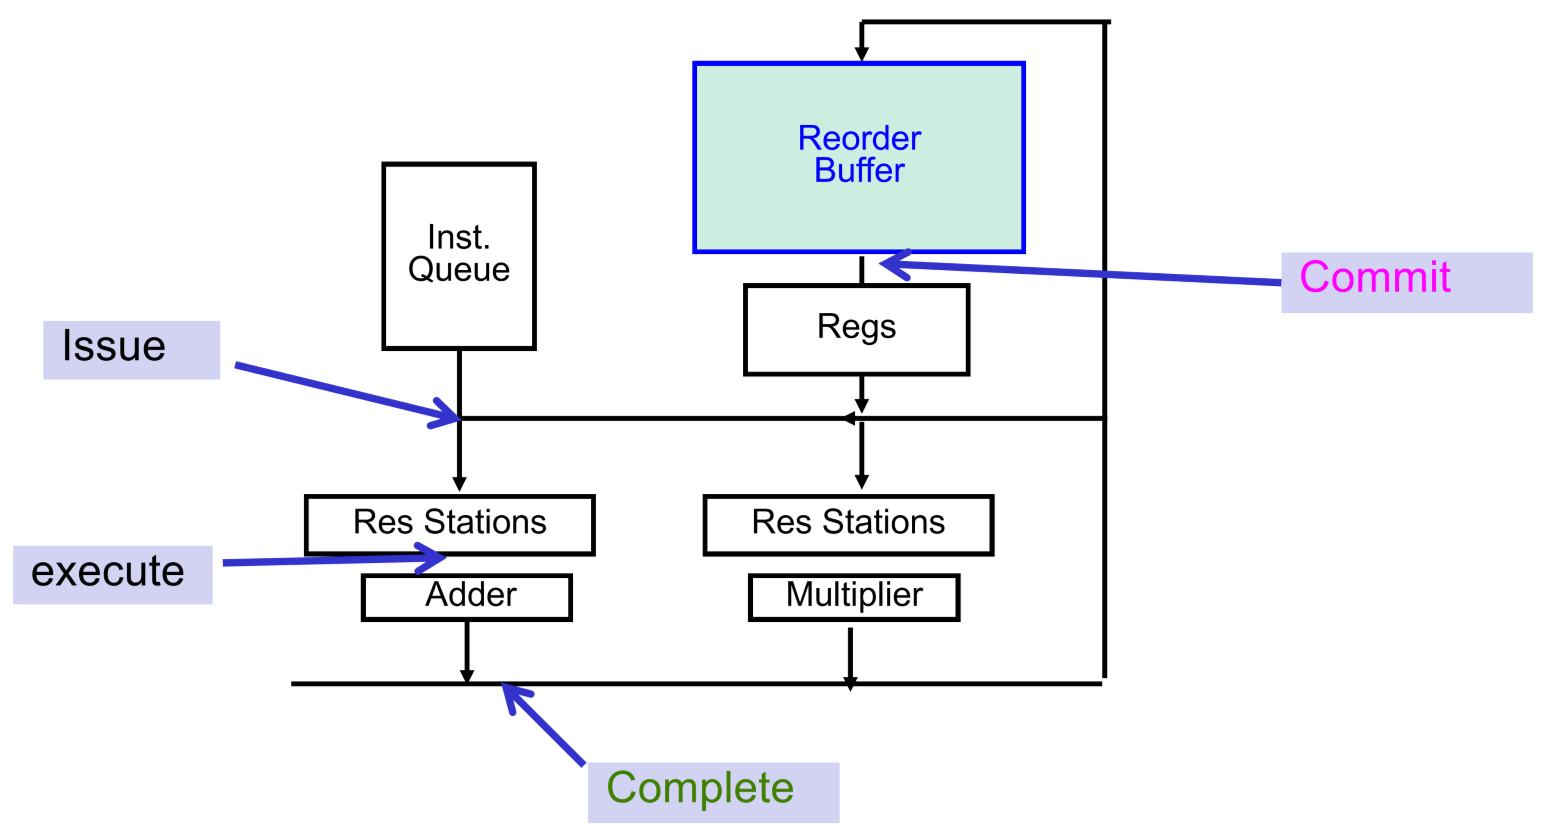
\includegraphics[width=100mm]{img/ROB.png}
\caption{Reorder Buffer}
\end{figure}

The reorder buffer can be quite long because while something like a conditional division is executing, we can predictively execute many instructions, but we have to store them before committing in case there's an exception. 

The issue stage allocates reservation stations and ROB entries. Here we keep track of the PC in case there's an exception or an mispredicted branch we need to continue from. We also keep track of the destination register to store the value in. We also need to keep track of which branch the instruction came from and whether it was speculative or not. That way even if we're at the head of the reorder buffer queue, we know not to commit it. 




\section{Instruction Set Architecture (ISA)}

The ISA is the interface between the operating system and the hardware. It is the language the computer understands and can execute. It can be thought of as a set of features visible to the programmer, and a contract that if the software is written in a certain way, the hardware can execute it.

All programming languages must be translated into the ISA for them to be executed. ARM is the ISA used on most mobile phones, and x86 is the architecture used on most laptops.

Processors now convert x86 instructions into RISC instructions and execute these in hardware. 

\subsection{Classifications of ISAs}

\subsubsection{Internal Storage}

\begin{enumerate}
\item \textbf{Stack} -- Operands are implicitly at the top of the stack

\item \textbf{Accumulator} -- One operand is implicitly the accumulator

\item \textbf{General-purpose register} -- All operands are explicit

\begin{enumerate}
\item \textbf{Register-memory} -- Can access memory as part of the operands in any instruction

\item \textbf{Register-register} -- Can access memory only with load-store instructions. 

Good because there's simple and fixed-length instruction encoding, so instructions take similar number of clock-cycles to execute which makes for easy pipelining. 

\end{enumerate}

\end{enumerate}

Now all architectures pretty much use register-register (also called load-store). It's a lot faster because when you use registers to hold variables, it reduces slow  memory traffic. This architecture also makes it easier for the compiler to generate efficient code. Because there is simple and fixed-length instruction encoding, instructions take a similar number of clock-cycles to execute, which makes it easy to pipeline.

However, register-register architectures also have higher instruction counts and lower instruction density, which leads to much larger programs. This isn't a big deal except in mobile devices and embedded applications, because smaller code means less memory which means less cost and less energy consumption.


%A.1%


\subsubsection{Number of Operands}

\begin{enumerate}

\item \textbf{Three operands} -- There is one result operand and two source operands

\item \textbf{Two operands} -- One of the operands is both the source and the result operand

\end{enumerate}

\subsection{Memory Addressing}

Memory is usually aligned in chunks of bytes, half-words, words, or double-words. Accesses to this memory has to be aligned as well. For each of these chunks it takes one memory reference to access it. For an object of $n$ bytes at byte address $A$, memory is aligned if

\begin{equation}
A\ mod\ s = 0
\end{equation}
\myequations{Memory Alignment}

When memory is misaligned it takes multiple memory references, so programs with aligned accesses are faster.

\subsection{Addressing Modes}

Addressing modes are how the instructions specify what address they want to access in memory. These are used to compute the \textit{effective address}.


\begin{table}[ht]
  \centering
  \caption{MIPS Addressing modes}
  \begin{tabular}{lll}
    \toprule
    \textbf{Mode} & \textbf{Example} & \textbf{Meaning}  \\
    \midrule
	Register & \texttt{Add R4, R3} & $R4 = R4+R3$ \\
	\textbf{Immediate} & \texttt{Add R4, \#3} & $R4 = R4+3$ \\
	\textbf{Displacement} & \texttt{Add R4, 100(R1)} & $R4 = R4+Mem[100 + R1]$ \\
	\textbf{Register Indirect} & \texttt{Add R4, (R1)} & $R4 = R4+Mem[R1]$ \\
	\textbf{Direct} & \texttt{Add R1, (1001)} & $R1 = R1+Mem[1001]$ \\
	\textbf{Memory Indirect} & \texttt{Add R1, @(R3)} & $R1 = R1+Mem[Mem[R3]]$ \\
	Autoincrement & \texttt{Add R1, (R2)+} & $R1 = R1+Mem[R2]; R2 = R2 +d$ \footnotemark \\
	Autodecrement & \texttt{Add R1, -(R2)} & $R2 = R2-d; R1 = R1+Mem[R2]$ \\
	Scaled & \texttt{Add R1, 100(R2)[R3]} & $R1 = R1 + Mem[100+R2+R3*d]$ \\

	\bottomrule
  \end{tabular}
\end{table}

\footnotetext{Here R3 would contain a pointer to another address.}

Some of these are very complicated, but the vast majority of addressing modes that are used by the compiler are simple addressing modes like Immediate (for constants), Displacement (for local variables), and some Register Indirect (for pointers). If designing an ISA, be sure to implement these commonly used modes.

\subsection{Control Flow}

\textit{Jumps} are unconditional changes in control, and \textit{branches} are conditional changes in control. These jumps are made by specifying the destination by giving the PC a relative displacement from the current location. Since the destination is usually close to the branch, the displacement relative to the PC takes fewer bits than an absolute address. It also means code can run regardless of where it is loaded. 

There are are also \textit{procedural calls} (\texttt{JALR}) and \textit{procedural returns} (\texttt{JR}) used for functions. These copy the PC to a register when the call is made, and then change the PC back to that to return to the saved address. This is called a dynamic address, which is good for methods in object-object oriented languages, because different routines can be called depending on the type of the argument.

\subsection{Encoding an Instruction Set}

The operation is specified in the \textit{opcode} field. 

\begin{enumerate}

\item \textbf{Variable-length} opcodes can support any number of operands and allows all addressing modes to be used with all operations. It also allows for the smallest code representation.

\item \textbf{Fixed-length} opcodes are easily pipelined and decoded by the hardware, and so will give better performance.

\end{enumerate}

\subsection{MIPS}

MIPS is designed to emphasize pipelining efficiency and efficiency as a compiler target, with the following features

\begin{enumerate}
\item \textbf{Load-store architecture}

\item \textbf{Fixed-length} encoding for good performance

\item \textbf{32} 64-bit GPRs and \textbf{32} floating-point registers, where \texttt{R0} is 0

\item Supports \textbf{immediate} and \textbf{displacement} addressing modes, where register indirect and absolute addressing are accomplished by using R0 

\item All memory access must be \textbf{aligned}

\item Floating-point operations use a \textbf{D-suffix} for double precision and \textbf{S-suffix} single

\end{enumerate}


\section{Pipelining}

Pipelining is a technique that overlaps multiple instructions. It's also invisible to the programmer, but presents many complications and performance benefits to the architect. Pipelining exploits parallelism by completing different parts of different instructions simultaneously. Each of these stages is called a \textit{pipe stage}, and each pipe stage usually takes one clock cycle to complete. 

For the best performance, each pipe stage should take the similar amounts of time to complete so that the clock cycle can be at a minimum without any stages sitting idle. 

\subsection{Classic 5-Stage Pipeline for a RISC Processor}

Every instruction in this RISC can be implemented in five clock cycles over five stages.

\begin{enumerate}
\item \textbf{IF, Instruction fetch} -- Fetch the current instruction from the memory location of the PC and put it into the instruction register (IR), then update the NPC to PC+4. 

\item \textbf{ID, Instruction decode} -- Decode the instruction in the IR, read the source registers, and compute the possible branch target address.

\item \textbf{EX, Execute} -- Send the operand values to the ALU and calculate the operation. In a memory operation, it would compute the effective address of the load/store. In a branch, the ALU adds the NPC to the offset and shifts it left by two.\footnote{The PC will always be a multiple of four, and multiple of fours always end with 2 zeros, so we don't actually save those two bits and we can just shift left by two later.}

\item \textbf{MEM, Memory access} -- If the instruction is a load, memory does a read from the effective address. If the instruction is a store, then the memory writes to the effective address. Update the PC with the NPC.

\item \textbf{WB, Write-back} -- Write the result to the destination register (the result comes from memory in a load, and from the ALU in other instructions)

\end{enumerate}

We overlap our instructions such that each pipe stage stays busy by starting the next instruction as soon as possible. The major functional units are used in different cycles, so each instruction can be executed independently.

\begin{table}[H]
\small
\centering
\caption{MIPS Pipelining Hazards}
\begin{tabular}{lccccccccc}
\toprule
\textbf{Clock cycle} 		& 1 	& 2 	& 3 	& 4 	& 5 	& 6 	& 7 	& 8 	& 9   	\\ 
\midrule
\texttt{DADD R1, R2, R3} 	& IF 	& ID 	& EX 	& MEM 	& WB  	& 		& 		& 		&  		\\
\texttt{DSUB R4, R1, R5} 	&		& IF 	& ID 	& EX 	& MEM 	& WB  	& 		& 		& 		\\
\texttt{AND  R6, R1, R7} 	&		&		& IF 	& ID 	& EX 	& MEM 	& WB  	& 		& 	  	\\
\texttt{OR   R8, R1, R9} 	&		&		&		& IF 	& ID 	& EX 	& MEM 	& WB  	&  	  	\\
\texttt{XOR  R10, R1, R11} 	&		&		&		&		& IF 	& ID 	& EX 	& MEM 	& WB  	\\
\bottomrule
\end{tabular}
\end{table}

Between each stage we have \textit{pipeline registers} to store the immediate values. In the first half of each clock cycle, these are written to by the preceding stage, and in the second half of the clock cycle, they are read the the following stage. These registers also carry intermediate values from one stage to another where the stage isn't needed. 

For instance, in a store instruction the value is read in ID but EX just passes it along to MEM.  Similarly, in an ALU instruction MEM just passes the value from EX to WB without doing anything in memory.

Pipelining increases the CPU instruction throughput, the number of instruction per time, but increases the amount of time it takes to complete each instruction because of pipeline register delay. The more balanced the stages, the better the performance because no stage is sitting idle.


\subsection{Pipeline Hazards}

Pipelining makes things a lot more complicated too. \textit{Hazards} are situations where one instruction is prevented from being executed in the pipeline until the previous instruction is complete. 

\begin{enumerate}

\item \textbf{Structural hazards} -- Resource conflicts when two instructions want to use the same hardware. For instance, you might only have one ALU and one instruction is the ID stage and wants to compute the effective address for the PC, while another instruction is in the EX stage and wants to do a subtraction. If this is the case, we has to \textit{stall} our next instruction until the hardware is free to use, or we could implement extra hardware.

\item \textbf{Data hazards} -- We also get issues where one instruction depends on a value computed or loaded by a previous instruction. If these instructions overlap, then the first instruction won't be done by the time the second instruction is reading its operands. 

\end{enumerate}


\subsubsection{Forwarding}

Data hazards can be mitigated by using forwarding, this way we can reduce the number of stalls.

The result of an ALU operation is known by the end of the EX stage. So an instruction that's dependent on that value doesn't need to wait until it's finished the MEM and WB stages. The result of a load operation is known by the end of the MEM stage, so we don't need to wait until the WB stage is completed. 

This requires some extra hardware called a \textit{pipeline interlock}. 

The values stored in the EX/MEM register or the MEM/WB register can be fed back to the ALU input directly. If we detect that the previous ALU operation will write to a register that is the source for a current ALU operation, then we know to forward. Control logic switches the ALU input to be from the forwarded result rather than the register file, and we don't have to stall.

If any of the source registers in the ID/EX or the EX/MEM registers are the destination registers in the EX/MEM or the MEM/WB registers, we know we should forward.

In the following case, in the ID stage the forwarding hardware detects the use of R1 in the \texttt{DADD}, and stalls the \texttt{DADD}.

\begin{verbatim}
LD   R1, 45(R2)
DADD R5, R1, R2
\end{verbatim}

In the following case, in the comparators again detect the use of R1 in the \texttt{DADD}, but can forward the load result to the \texttt{DADD}.

\begin{verbatim}
LD   R1, 45(R2)
DSUB R3, R6, R7
DADD R5, R1, R2
\end{verbatim}

\subsubsection{Branch Hazards}

\textit{Control hazards} can cause worse performance than our data hazards. 

When a branch is executed it could either be \textit{taken} and increment the PC by some offset to the target address, or it could be \textit{not taken} and increment by four to go to the next instruction. If the instruction is taken, it will update the PC at the end of the ID stage. 

The next instruction will be stalled for one cycle until the IF stage knows what instruction to fetch from the updated PC. One stall for every branch will have a significant performance loss.

Alternatively, you could assume all branches are not taken and before you know the target address if taken or even if it is taken, you can begin to execute the next instruction as if the PC was incremented by four. If the branch is not taken, continue as normal. If it is taken, you must be able to back out by converting the instruction to a NOP and ensure that nothing has been irreversibly changed and you haven't lost any register values or anything.

As pipelines get deeper, the penalties of taking the wrong branch increases. 

\begin{equation}
SU_{pipeline} = \dfrac{Pipeline\ depth}{1 + Branch\ frequency \times Branch\ penalty}
\end{equation}
\myequations{Pipeline Speedup of branch schemes}

\textit{Static branch prediction} uses information at compile-time to bias branches towards taken or untaken. The misprediction rate is higher for integer operations than floating-point operations.


\textit{Dynamic branch prediction} uses run-time information to make informed predictions. A \textit{branch history table} is created that hashes the lower portion of the instruction address to a bit that indicates whether the branch was taken last time or not. 

A one bit scheme will make two mispredictions per loop even if a branch is almost always consistently taken or not taken. By increasing it to two bits, and implementing a policy that we must mispredict twice in a row before changing our assumption, we reduce this to one misprediction per loop.

Another indicator of the accuracy is the number of branches and their histories that we can save in our branch history table. A table with 4000 entries performs comparably to an infinite buffer for SPEC benchmarks.

\subsection{Pipeline Control}

Control of the pipeline is done through multiplexers. 

\begin{enumerate}
\item \textbf{ALU mux in EX} -- Two multiplexers go into the ALU to specify the instruction type in the IR. 

\item \textbf{PC mux in IF} -- This mux is set based on if the instruction is a branch. If it is, the PC is incremented by the offset calculated in the EX stage, otherwise it is incremented by 4.

\item \textbf{Memory mux in WB} -- This mux is set by whether the instruction is an ALU or a load operation. Branch and store instructions don't need to write back any results to the register file.

\end{enumerate}

%Fig. C.22%

An instruction is \textit{issued} when it is moved from ID to EX. All data hazards can be checked during the ID stage, and issued only when they are resolved. Likewise, we can determine what forwarding is needed during the ID stage and set the appropriate controls.

When a hazard is detected, we can change the control portion of the ID/EX pipeline register to all 0s to simulate a no operation, and we recirculate the IF/ID register back itself to try again. 

\subsection{Exceptions}

Exceptions, also called \textit{interrupts} and \textit{faults} are situations where the normal execution is changed. These include divides by zeros, segmentation faults, debugger breakpoints, and page faults.

These are hard to deal with in pipelines because the overlapped instructions  make it hard to stop exactly at one instruction that's causing the problem.

We can categorize these in various ways

\begin{enumerate}
\item \textbf{Sync vs. async} -- Synchronous exceptions happen at the time place every time the program is executed. Most exceptions other than hardware failures and external interrupts are synchronous. Asynchronous exceptions are usually easier to handle because they can be dealt with after the completion of the current exception.


\item \textbf{User maskable vs. user non-maskable} -- This indicates whether or not the exception can be ignored. A maskable interrupt can indicate that the hardware doesn't need to respond the the event. 

\item \textbf{Resume vs. terminate} -- If the program always stops after the interrupt, it's a terminating event. Resume events can continue after the interrupt. It's easier to have a terminating event because you don't have to deal with restarting the program.

\end{enumerate}

By the time the exception happens, a few instructions could be in flight. The pipeline state and the PC must be saved and shut down so that it can be restarted after the exception has been fixed.

We have a \textit{precise exception} if when the pipeline is stopped at the exception, all the preceding instructions are completed and all the following instructions are flushed. Precise exceptions run much slower and are only really useful for debugging.

\subsection{Multicycle Operations}

Before we assumed that the EX stage took only one cycle. Floating-point operations take many cycles to complete. We cannot make all instructions take the same amount of time, because then we'd have extremely deep pipelines, or a slow clock, or massive amounts of logic, and our stalls would be very long.

For these instructions the EX cycle is repeated until the operation is complete. There also are multiple function units (FUs), one for integer operations, one FP and integer multipliers, on FP adder, and one FP divider. Each of these FUs has different latencies.

%Fig C.32%

These functional units are split into microinstructions (M1, M2, M3... for multiplication and A1, A2, A3... for addition) which can then also be pipelined. This requires additional pipeline registers called (M1/M2, M2/M3...).

\begin{figure}[ht!]
\centering
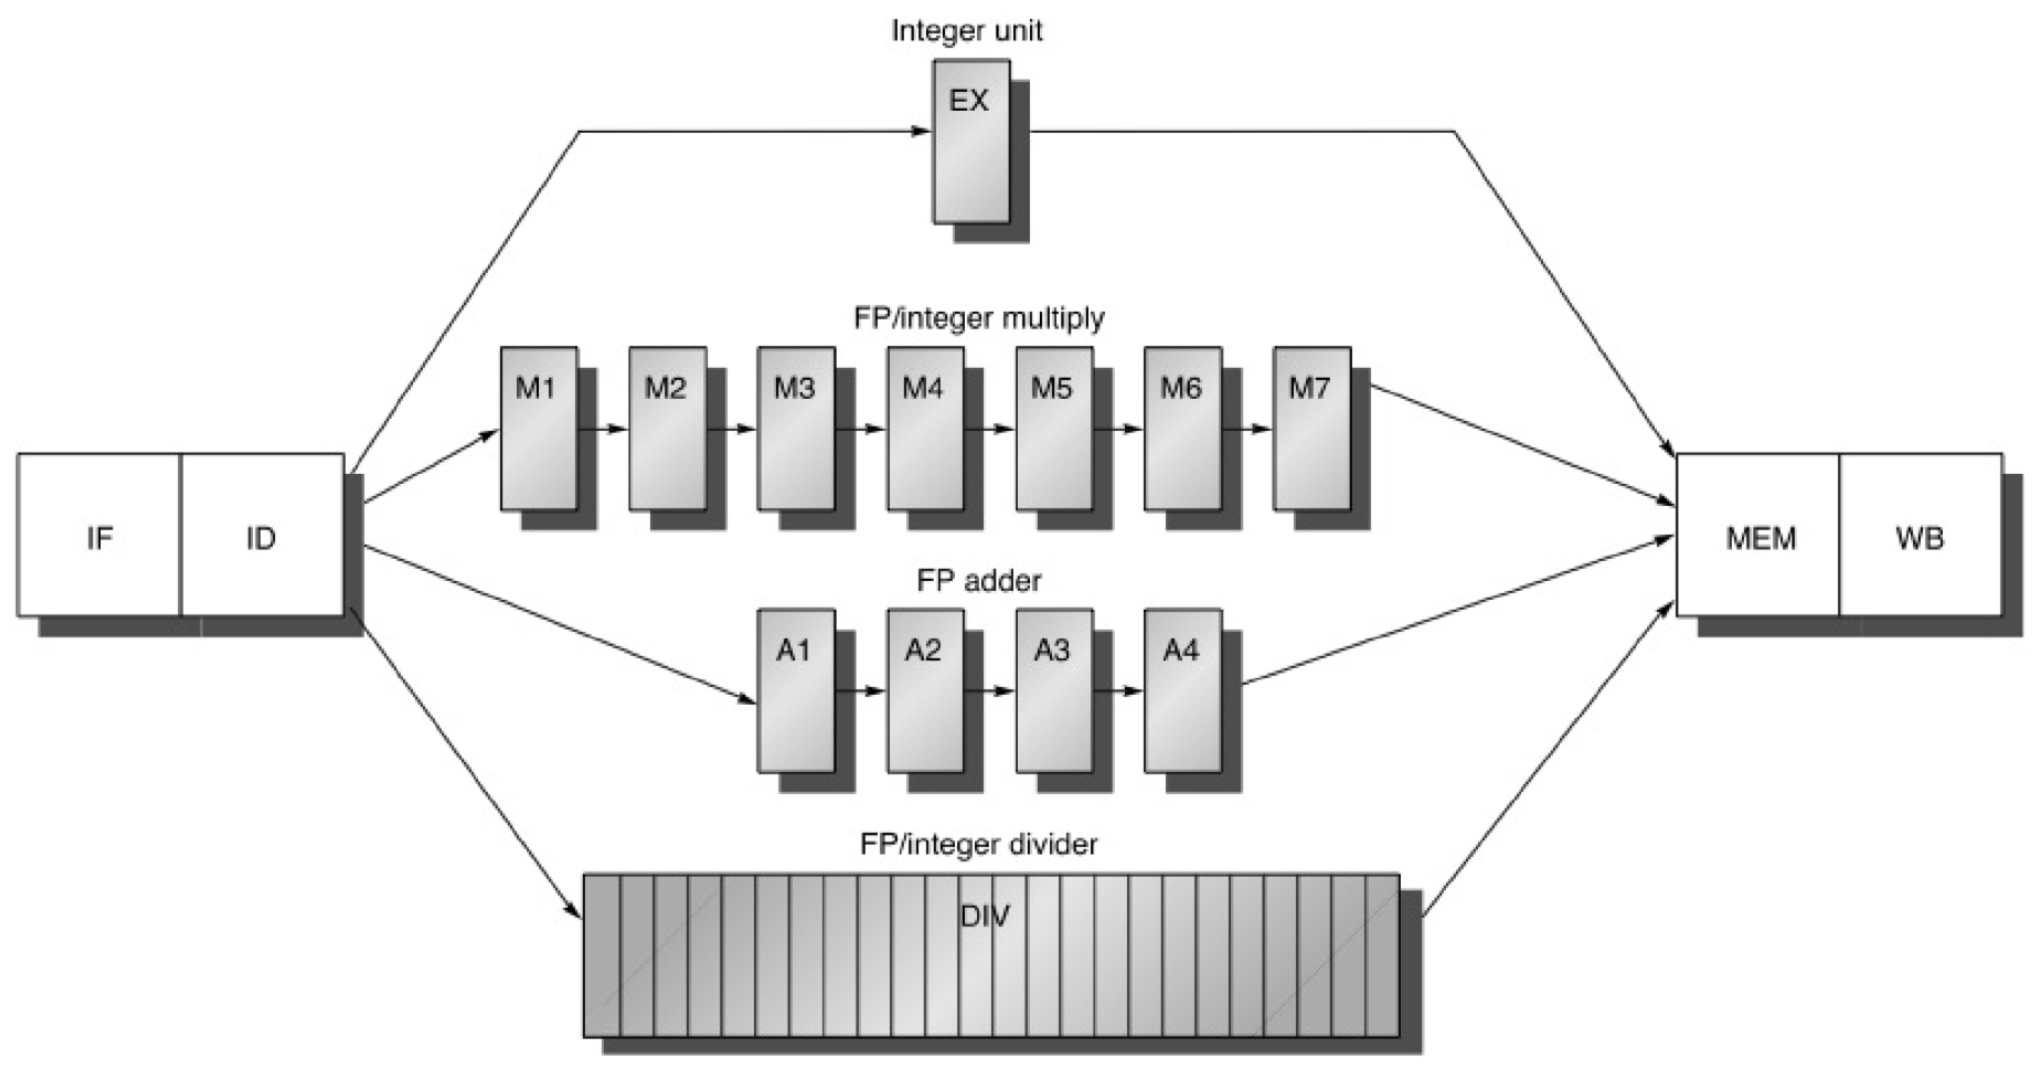
\includegraphics[width=120mm]{img/PipelinedFU.png}
\caption{Multicycle Operations}
\end{figure}

Because these operations take different amounts of time to complete, we get \textit{out-of-order completion}. A multiplication instruction that begins before a load instruction can complete after the load completes. These are new hazards. 

\subsubsection{Hazards and Forwarding in Longer Latency Pipelines}

Because these instructions take more than five cycles to complete, stalls have a much greater penalty and RAW hazards will become more frequent. 

%Fig. C.37%

This also introduces a new hazard, \textit{write-after-write} (WAW). Since instructions don't reach the WB stage in order, a later instruction writing to register R1 could complete before a previous instruction writing to register R1. This means that the intended value stored in R1 would be overwritten. These hazards only occur when an instruction that didn't need to be executed is completed, because it will be overwritten anyway. However, these instances happen, for instance at the end of a loop right before the loop is exited. 

We can deal with WAW hazards by detecting them in the ID stage and either stalling the second write until the first write is completed, or recognizing the first write is useless and converting it to a NOP. 

\textit{Write-after-read}(WAR) instructions are not an issue however, since the register reads always occur in ID which are executed in order.

Also, different FUs may complete their execution in the same clock cycle, and both try to WB or MEM at the same time. These create structural hazards, for instance if there is only one write port to the register file.


There are three checks we must do with pipelined functional units:

\begin{enumerate}
\item \textbf{Check for structural hazards} -- Wait until the required FU is not busy and make sure the write point will be available when needed

\item \textbf{Check for a RAW data hazard} -- Wait until the source registers for the operation are not listed as pending destination registers

\item \textbf{Check for a WAW data hazard} -- Determine if any instruction in flight has the same destination register as the operation
\end{enumerate}

The other side effect is that because instructions are completed out of order, dealing with exceptions will be complicated. More on that later.

\subsubsection{Maintaining Precise Exceptions}

Consider the following instructions

\begin{verbatim}
DIV.D  F0,  F2,  F4
ADD.D  F10, F10, F8
SUB.D  F12, F12, F14
\end{verbatim}

The \texttt{ADD.D} will complete before the \texttt{DIV.D}, but then suppose we start the \texttt{SUB.D} instruction and it causes an exception. Then we will have to roll back to where we were before the \texttt{DIV.D}, but the \texttt{ADD.D} will have destroyed the previous F10 value. 

This problem occurs because of out-of-order completion and it complicates our ability to have precise exceptions. We can deal with it in a few ways

\begin{enumerate}
\item \textbf{Settle for imprecise exceptions}

\item \textbf{Buffer the results} until we know all the operations issued earlier are completed

\item \textbf{Buffer the results} until we know all the operations issued earlier will complete without an exception
\end{enumerate}


\subsection{Dynamically Scheduled Pipelines}


Simple pipelines fetch an instruction and then issue it unless it is dependent on another instruction already in the pipeline. They stall the instruction until the dependency can be forwarded. 

But let's say the instruction following the one being stalled isn't dependent on the value we're stalling for. Then we have head-of-the-line blocking and we're not using hardware that could otherwise be put to use. 

With \textit{dynamic scheduling} the hardware rearranges the instruction execution to minimize stalls. We can do this, with a \textit{scoreboard}. So far we've only talked about in-order issue, which means that if an instruction is being stalled, no subsequent instructions can be issued. 

We still decode and issue instructions in order, but we will execute instructions as soon as their operands are available -- this is called \textit{out-of-order execution}. To do this we split the ID pipe stage into

\begin{enumerate}
\item \textbf{Issue} -- Decode instructions and check for structural hazards

\item \textbf{Read operands} -- Wait until no data hazards then read operands
\end{enumerate}

\subsubsection{Scoreboard}

In a dynamically scheduled pipeline, all instructions pass through the issue stage in order, however in the read operands stage they can be stalled and leapfrog each other, thus be executed out of order. Scoreboarding helps us know when we can do this. 

Previously WAR hazards didn't appear, but now that we can execute out of order, we have to consider them. Consider this code

\begin{verbatim}
DIV.D  F0,  F2,  F4
ADD.D  F10, F10, F8
SUB.D  F8,  F12, F14
\end{verbatim}

If the \texttt{SUB.D} instruction is executed before the \texttt{ADD.D} instruction, then the \texttt{ADD.D} will read the wrong value of F8. We also still have to consider WAW hazards, for the same reason.

The point of a scoreboard is to continue executing instructions as early as possible when there aren't hazards. Out-of-order execution requires using our multiple functional units. 

Every instruction goes through the scoreboard in the issue stage and a record of the data dependencies is constructed. The scoreboard determines when the instruction's operands will be available and schedules it to start that cycle. It also controls when an instruction can write its result to the destination register. 

This takes four steps

\begin{enumerate}
\item \textbf{Issue} -- If a FU is free (no struct. hazards) and no other active instruction has the same dest. register (no WAW hazard), issue the instruction. Otherwise stall it.

\item \textbf{Read operands} -- If no instruction in flight is going to write to one of our operand registers (no RAW hazards), then begin execution. Otherwise stall it. It's here that instructions can be executed out-of-order.

\item \textbf{Execution} -- The FU gets its operands, calculates, and notifies the scoreboard when it's done.

\item \textbf{Write result} -- Once the scoreboard knows the FU is done, it checks that no instruction is currently waiting to read the register we're going to write to (no WAR hazard) and writes the result. Otherwise it stalls.

\end{enumerate}

There are three parts to the scoreboard

\begin{enumerate}
\item \textbf{Instruction status} -- Indicates which step the instruction is in

\item \textbf{FU status} -- Indicates the state of the FU. There are nine fields.

\begin{enumerate}
\item \textit{Busy} -- a bit to indicate if busy or not

\item \textit{Op} -- what operation is being performed

\item \textit{$F_i$} -- what the destination register is

\item \textit{$F_j,\ F_k$} -- what the source registers are

\item \textit{$Q_j,\ Q_k$} -- what FUs are going to produce the source register contents

\item \textit{$R_j,\ R_k$} -- whether the source registers are ready to read and haven't been read 
\end{enumerate}

\item \textbf{Register result status} -- This keeps a list of each register and which FU will write to that register if the register is pending on an instruction
\end{enumerate}


The effectiveness of a scoreboard depends on how many instructions are independent and can be parallelized, how many entries we can store in the scoreboard (the window size), the number of functional units we have to use simultaneously, and how many WAR and WAW hazards there are in the code.


\section{Instruction-Level Parallelism}


\subsection{Advanced Branch Prediction}

Branch predictors predict whether to take or to not take a branch. 

The target PC is different from the instruction at the memory location pointed to by the PC. The PC is the address of memory location containing the next instruction, whereas the instruction is just the opcode and registers of the next instruction.

So if branch predictors predict whether to take the branch, the Branch Target Buffer (BTB) is a cache that predicts the target PC assuming the branch is taken.

The first time you see a branch, you stick the address (or a component of the address) of the branch in the tag component of a BTB row. After you resolve the branch, you put the address of the location we branched to in the target component. Next time we come to that address, if the branch is predicted as taken, we can predict the location where to branch to without resolving it. 

As we increase the number of instructions in flight, the accuracy of our branch prediction becomes more important. One way that we can improve our prediction scheme over the 1 or 2-bit predictor we discussed earlier is to take into account \textit{correlating branches}. 

Correlating branches are branches for which the outcome depends on one-another, for instance consider this code in the eqntott benchmark. 

\begin{verbatim}
if (a == 2) a = 0;
if (b == 2) b = 0;
if (a != b) ...
\end{verbatim}

Here, if the first two if statements are executed then the last if statement will not be executed. When compiled into MIPS, this means that when the branches b1 and b2 are taken, then b3 will be taken (note that the logic for true corresponding to taken may be inverted by the compiler to bias the code one way or another). 

Branch predictors may use the global behaviour of other branches to make predictions. This is done by looking at a history of recently executed branches. An $(m,\ n)$ predictor looks at the behaviour of the last $m$ branches to choose from $2^m$ branch predictors, each of which is an $n$-bit predictor for a single branch. 

The 2-bit saturating counter we discussed previously is a $(0,\ 2)$ predictor because it doesn't use any history of previously executed branches (meaning different branches, not this same branch executed a previous time), and it uses a 2-bits history to make its prediction.

A $(2,\ 2)$ correlating predictor outperforms a 2-bit saturating predictor not only with the same total number of bits, but with an unlimited number of entries.


\subsection{Dynamic Scheduling using Tomasulo's Algorithm}

In-order instruction issuing creates head-of-the-line blocking, as we have discussed earlier. With out-of-order execution we can execute non-dependent instructions while dependent instructions are stalling. However, recall that this introduces WAR and WAW hazards. 

It also complicates preserving precise exceptions, because instructions after the exception may have already been completed, and instructions before the exception may not have been completed. 

Previously we discussed dealing with this using scoreboarding, which allowed us to execute out-of-order when there were no structural hazards and there were no data dependencies. 

A more sophisticated technique of dealing with this is using \textit{Tomasulo's algorithm}. This eliminates WAW and WAR hazards by using dynamic \textit{register-renaming}. Recall these hazards only arise through reusing registers. 

RAW hazards are avoided by executing only when its operands are available, similar to the scoreboarding technique. 

\subsubsection{Register-renaming}

Register-renaming is provided by using \textit{reservation stations}. 

Reservation stations buffer the operands of instructions waiting to be issued. This way, an operand is fetched and buffered in the reservation station as soon as it is available. This way it doesn't need to be fetched from a register, and the register can be overwritten. As instructions are issued, the source registers are renamed to the corresponding reservation station tags.

This way we can forget about registers and just track data dependencies directly. Each destination register gets a new tag, and that tag is mapped to in the \textit{register alias table} (RAT). These tags are basically an extended set of virtual registers.

All results from the FUs are broadcast on the \textit{common data bus} (CDB), so all FUs waiting for an operand can load the result simultaneously. 

Each FU has a reservation station that holds an issued instruction waiting to be executed until the operands are available. 

Instructions are sent to the instruction queue, which will issue them in order. When the instructions are issued, they will be sent to reservations station which will hold the operation and the operands. 

The load and store buffers hold data or addresses coming from and going to memory until the effective address is computed. They behave almost exactly like reservation stations.


%Fig. 3.6%


There are three steps to the algorithm

\begin{enumerate}
\item \textbf{Issue} -- Get the next instruction from the head of the queue. 

\begin{itemize}
\item If there is an available reservation station for the FU (no struct. hazard), issue the instruction to that reservation station. 

\begin{itemize}
\item If the instruction's operands are in registers that aren't in flight, pass the values to the reservation station.

\item If the instruction's operands aren't available, track the FUs that will produce the result and pass the tags. (This eliminates WAR and WAW hazards).
\end{itemize}

\item If there isn't an available reservation station, stall until a station or a buffer is free.
\end{itemize}

\item \textbf{Execute} -- If any operands aren't available and you have their tags, listen for them on the CDB. When they become available, put it in the reservation station that's waiting for them. Once all operands are available, begin executing.

\begin{itemize}
\item To preserve precise exceptions, no instructions are allowed to execute until all branches before it have been completed. When using branch prediction,this means we have to know the branch prediction was correct before beginning execution.
\end{itemize}

\item \textbf{Write result} -- When the result is available, write it and the destination tag on the CDB. Any registers or reservation stations waiting on the result will see the matching tag and update their value

\end{enumerate}

The reservation stations have the following fields:

\begin{enumerate}

\item \textit{Op} -- what operation is being performed on the source operands 

\item \textit{$Q_j,\ Q_k$} -- the reservation stations that will produce the source operands (a value of zero means we already have the value in $V_j$ or $V_j$)

\item \textit{$V_j,\ V_k$} -- the values of the source operands

\item \textit{$A$} -- used to hold effective address calculated for loads or stores

\item \textit{$Busy$} -- if this reservation station's FU is free

\end{enumerate}

One of the main benefits of Tomasulo's algorithm is that if multiple instructions are waiting on a single result, since the result in broadcast on the CDB, both instructions can start simultaneously. If the result was going to a register file, then the instructions would have to fetch the value one at a time. 

The second is that we eliminate WAW and WAR hazards. For instance, consider the following code: 

\begin{verbatim}
L.D     F6,  32(R2)
L.D     F2,  44(R3)
MUL.D   F0,  F2,  F4
SUB.D   F8,  F2,  F6
DIV.D   F10, F0,  F6
ADD.D   F6,  F8,  F2
\end{verbatim}

We can issue both the \texttt{DIV.D} and the \texttt{ADD.D} even though they have a WAR hazard on F6. 

If the value of F6 has been loaded, then its value has been stored in the reservation station for the \texttt{DIV.D}, so even if the \texttt{ADD.D} executes before the \texttt{DIV.D} and overwrites F6, we won't lose the previous value.

If the value of F6 has not yet been loaded, then the \texttt{DIV.D} reservation station would point to the result of the load FU and wait for it, and grab the value regardless if \texttt{ADD.D} is overwriting the F6 register.

\subsection{Hardware-Based Speculation}

Hardware speculation expands on dynamic scheduling. In dynamic scheduling you only fetched and issued speculatively, you waited until you knew you speculated correctly before beginning execution. Now we will fetch, issue, and \textit{execute} as if our branch predictions are always correct. Operations will now execute as soon as their operands are available. 

We also need to be able to handle the situation and revert when our speculations are incorrect. 

Hardware-based speculation requires the following tools we have discussed so far

\begin{enumerate}
\item Dynamic branch prediction

\item Speculatively execute instructions before control dependencies are resolved

\item Ability to undo the effects of an incorrectly speculated branch

\item Dynamic scheduling to overlap executions
\end{enumerate}

We now extend Tomasulo's algorithm to allow an instruction to execute and forward its results, without actually performing any updates that can't be undone until we know we made the right prediction. This is like doing a speculative register-read. 

When the branch is resolved and we know we made the right prediction, we can update the register file or memory in an \textit{instruction commit}. This allows us to execute out-of-order, but prevent any irrevertable changes by \textit{committing in-order}. 

We implement this change by incorporating the \textit{reorder buffer} (ROB). This provides additional registers like a reservation station, and it holds the result of an instruction after it is executed but before it is committed. It is a source of operands for instructions just like the reservation station. 

Each entry in the ROB contains the following.

\begin{enumerate}
\item \textbf{Instruction type} -- indicates whether it's a branch, a store, or a register operation

\item \textbf{Destination field} -- the destination register number for loads/ALU operations, or the destination memory address for stores

\item \textbf{Value field} -- holds the value of the instruction result until ready to commit 

\item \textbf{Ready field} -- indicates whether the instruction has completed execution and has a value
\end{enumerate}

%Fig. 3.11%


The execution steps in hardware-based speculation are the following.

\begin{enumerate}
\item \textbf{Issue} -- Get the next instruction from the head of the queue. Issue the instruction if there is an empty reservation station and an empty slot in the ROB.

\item \textbf{Execute} -- If any operands aren't available and you have their tags, listen for them on the CDB. When they become available, put it in the reservation station that's waiting for them. Once all operands are available, begin executing.

\item \textbf{Write result} -- When the result is available, write it on the CDB with the ROB tag. Load the result into the ROB and any registers or reservation stations waiting on it. 

\item \textbf{Commit} -- For non-branches and non-stores, when an instruction reaches the head of the ROB and its result is present, it updates the register and the instruction is removed from the ROB. For branches with incorrect prediction, when the instruction reaches the head of the ROB, the ROB is flushed because the subsequent instructions are wrong and execution is restarted. If the branch was correctly predicted, we continue.

\end{enumerate}

(???) How do we know the branch was correctly predicted? 

One advantage of the ROB is now the processor can dynamically and speculatively execute code while maintaining a precise exception model, because we only commit instructions in-order. If there are any mispredictions or exceptions, the processor can undo all actions by not committing if the instruction is found to be a misprediction or an exception. 

We still have the benefit of avoiding WAW and WAR hazards because actual updating of memory occurs in order. When an instruction is at the head of the ROB, no earlier instructions can still be pending. 

RAW hazards are still avoided through stalls. 

\newpage
\section{Caches}

How important are Caches? Well, take a look at the Intel Broadwell processor and look how much area is devoted to caches. Indeed, some of the area inside the cores are also caches, so caches are a huge component of modern processors.

\begin{figure}[ht!]
\centering
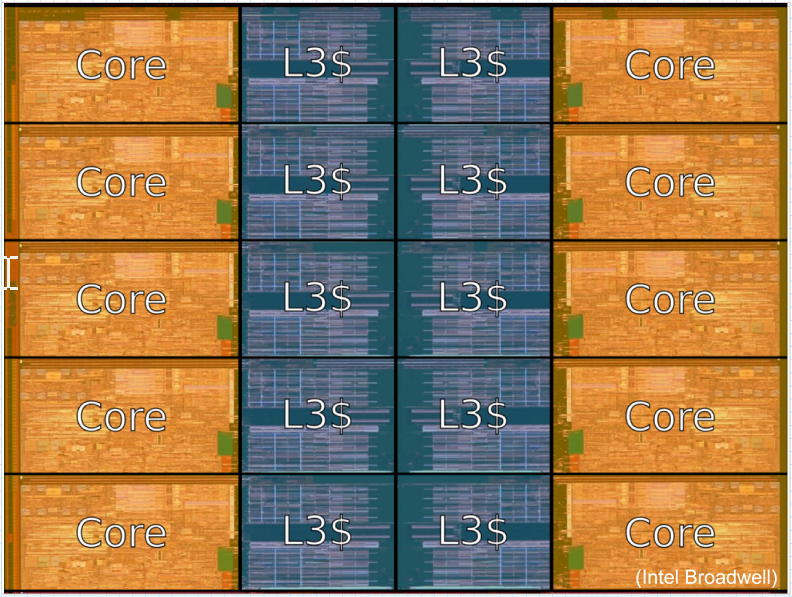
\includegraphics[width=80mm]{img/Cache.png}
\caption{Caches in an Intel Broadwell}
\end{figure}

We know how to create a CPU that can is pipelined, can execute instructions out of order and simultaneously, but we now need to connect it to memory. The latency of DRAM nowadays is around 51ns. When looking at Iron Law, $time = \#\ insts. \times CPI \times clk\ cycle$, we know latency affects the CPI. 

\subsubsection*{Example}

If using a 4GHz CPU with a DRAM latency of 51ns, what is the average CPI if every fifth instruction is a memory operation?

---

Assume non-memory operations take one cycle, which is $\frac{1}{4GHz} = 0.25ns$.

Memory operations take 1-cycle for the address calculation then take 51ns for the DRAM latency, which is $1 + \frac{51ns}{0.25ns} = 205\ cycles$. 

So the $average\ CPI = \dfrac{4}{5}1\ cycle + \dfrac{1}{5}205\ cycles = 41.8\ cycles$.

---

So this DRAM latency really brings up our average CPI. Even though we have a fancy and expensive CPU, but our CPI is still way higher than we want it to be. This is fixed using caches.

\subsection{Available Technologies}

\begin{enumerate}
\item \textbf{DRAM} -- Dynamic RAM is dense and cheap. Each DRAM cell only consists of one transistor and capacitor. However, it is slow, taking tens of ns.

\item \textbf{SRAM} -- Static RAM uses about five times more area per bit than DRAM because each cell is six transistors. But it's much faster.

Also the size of the SRAM corresponds to how fast it is. Small SRAMs are faster than larger SRAMs. For instance, 4KB of SRAM takes about 0.2ns per access whereas 32MB of SRAM takes about 5ns per access\footnote{At 32nm}.

\end{enumerate}

This gives us a tradeoff between big memories or fast memories. To optimize our performance with this tradeoff, we will use a memory hierarchy. 

\begin{enumerate}
\item \textbf{CPU} -- The CPU and its registers are at the top of the hierarchy

\item \textbf{L1\$} -- The level 1 cache is the smallest but fastest cache, directly connected to the CPU. It is about 32KB, 8-way (which we will discuss later), it's private to one core, and takes 4 cycles per access.

\item \textbf{L2\$} -- This cache is larger but slower at 256KB, 4-way, private to one core, and 12 cycles per access.

\item \textbf{L3\$} -- The largest cache is 8MB, 16-way, shared among multiple cores, and takes 42 cycles per access.

\item \textbf{Off-chip DRAM} -- This is 16GB+, per access it takes 42 cycles to go through the hierarchy plus 51ns of latency, so roughly 246 cycles.
\end{enumerate}



\begin{figure}[ht!]
\centering
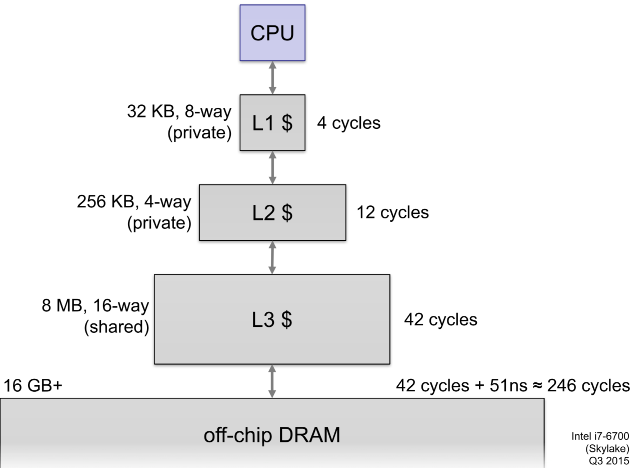
\includegraphics[width=100mm]{img/CacheHierarchy.png}
\caption{Cache Hierarchy}
\end{figure}

The point of the cache is to filter some of the accesses so we don't have to go through the whole hierarchy. 

\subsection{What to Keep in a Cache}

You want to keep things that you will frequency use in a cache. But to figure out what is frequently used, we'll run a simulation to learn how programs behave. Take a look at this \verb|SAXPY| loop from a single-precision gaussian elimination algorithm from a matrix multiplication library.

\begin{verbatim}
void saxpy(float a, float *X, float *Y, unsigned N)
{
   for(i=0; i < N; i++)
      Y[i] = a*X[i] + Y[i];
}
\end{verbatim}

First observe that we read \verb|Y[i]| before then writing to it. This is called \textit{temporal locality} -- meaning you're reusing a value that you used recently. 

If a program access a memory location then accesses it soon thereafter, there is a temporal locality.

The line \verb|Y[i] = a*X[i] + Y[i];| in assembly is the following:

\begin{verbatim}
L.S    F1, 0(R1)    ; read X[i]
MUL.S  F2, F1, F0   ; a*X[i]
L.S    F3, 0(R2)    ; read Y[i]        here we load from 0(R2)
ADD.D  F4, F2, F3   ; a*X[i] + Y[i]
S.S    F4, 0(R2)    ; write Y[i]       here we store to 0(R2)
\end{verbatim}

We can use caches to take advantage of temporal locality. Since we are going to be reusing data we have recently accessed, we can keep a copy of it nearby in small, fast memory.

Second observe that in our loop we access \verb|X[0]| then \verb|X[1]| then \verb|X[2]| and so on. This is called \textit{spatial locality} -- once we access one location, the program may attempt to access a nearby location.



But how do you know what to keep a copy of? There are two options.

\begin{enumerate}
\item \textbf{Scratchpad} -- We ask the programmer to figure out what the most useful data is and manually keep a copy. The program is given access to big and slow and small and fast memories and the program does all the work of figuring out what to save where. This is used in GPUs. 

This means the code has to change when the hardware changes and it is a lot more effort, but we could also be very clever and optimize exactly what memory to keep track of.

\item \textbf{Cache} -- We detect all localities automatically in hardware and manage what we should keep copies of. This is done transparently to the programmer and they don't need to worry about it. This is used in most CPUs and GPUs.
\end{enumerate}


\subsubsection{Temporal Locality}

What do we need to keep in the cache? 

Let's first look at the case of a Fully Associative Cache -- a cache which has to look in every entry to see if the data is there. Most importantly we need to keep the data in the cache. The valid bit indicates if the cache row actually has any useful data in it. We also need to know whether the data has been modified so we know if we need to write back our cache data. We also need to keep the tag in order to identify what data we have stored. 

\begin{figure}[ht!]
\centering
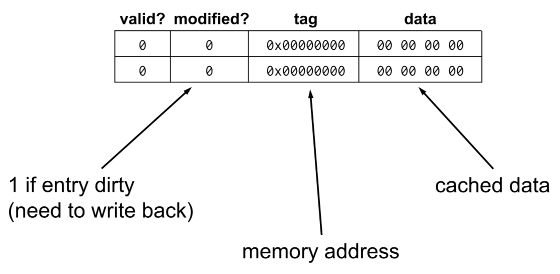
\includegraphics[width=100mm]{img/FAC.png}
\caption{Fully Associative Cache}
\end{figure}

\subsubsection*{Example}

Show the contents of a fully associative data cache after executing the following code, where initially \verb|R2=0x8| and \verb|F2=78.2|.

\begin{verbatim}
L.S    F3, 0(R2)
ADD.S  F4, F2, F3
S.S    F4, 0(R2)
\end{verbatim}

And the initial cache state and memory state is as follows:

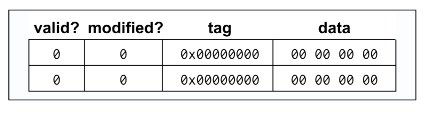
\includegraphics[width=80mm]{img/Miss.png}


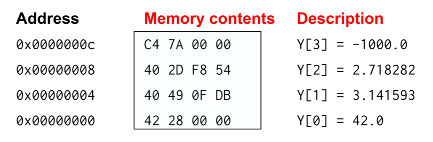
\includegraphics[width=80mm]{img/MemoryState.png}


---

The first instruction is a load, so first have to compute the effective address. Since \verb|R2=0x8|, then \verb|0(R2)=0x8|. Then we have to check if \verb|0x8| is already in the cache. Since there is nothing in the cache with that tag, we have a  \textit{miss}. So we have to read the data from memory, then we put it in F3 and also keep a copy of it in the cache\footnote{This is actually why misaligned memory data is so bad. One part of line of memory might be stored in the cache, but the other line isn't, so you don't have full misses or full hits. Or even two misses instead of one.}.

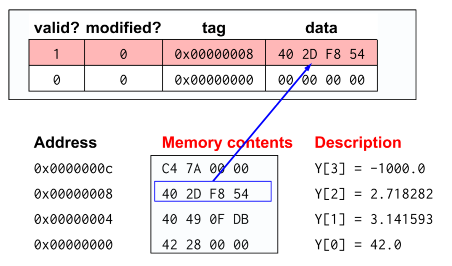
\includegraphics[width=80mm]{img/Update.png}

The third instruction is a store. Our new value of F4 from the previous add instruction must be put in the cache. Look in the cache to see if you have the tag corresponding to the store, and if so then update the data and set the modify tag to one.

Whether to now update the value in memory as well is a design choice called "writethrough", which we will come to later.




\subsubsection{Spatial Locality}

This is the other kind of locality we can consider. Programs are fairly predictable in that they do the same thing over and over again, and both of the kinds of locality are very predictable. If you access data in one place, then you may also be interested in data nearby. For instance, look at the following code.

\begin{verbatim}
Y[2] = a*X[2] + Y[2];
Y[3] = a*X[3] + Y[3];
\end{verbatim}

First we read \verb|Y[2]| then \verb|Y[3]|. Perhaps when we cache the value of \verb|Y[2]|, we then could also transfer a bigger chunk adjacent data. This way, we would not have to go into memory when we go to access \verb|Y[3]|. We will call these bigger chunks \textit{cache blocks}.

Memory is divided into blocks that are aligned in memory. In CPUs, a typical block size is 64-bytes and in GPUs it is 128-bytes. 

To do this we will have to change our cache. We will expand the data to contain an entire block rather than one memory location. We could also make our tag shorter as we only need to identify the blocks, not the memory address. 

The lower $log_2(block\ size)$ bytes of the memory address in an instruction simply identify the location within the block. For instance, with a fully associative cache of 8-byte blocks, the last 3-bits are dedicated to identifying the memory address within the block. So if the address we're interested is address \texttt{8}, then the tag in the cache is \texttt{0x0000001}, because we drop the lowest three significant bits.


\begin{figure}[ht!]
\centering
\includegraphics[width=70mm]{img/BlockOffset.png}
\caption{Block Offset}
\end{figure}

When the memory address is \texttt{0x0000001XXX} is accessed, the bits \texttt{XXX} identify the location within the block in the cache -- called the \textit{block offset}.

\subsubsection*{Example}

There is a data cache with 16 byte blocks, and a 4-byte float starting at address \texttt{0x00008028}. What is the block offset?

---

The number of bits devoted to the offset is $log_2(16) = 4\ bits$. The tag is therefore \texttt{0x0000802} and the offset is \texttt{0x8 = 0b1000}.

---

\subsubsection{Direct Mapped Cache}

They're very big because you have to store each entry and have to store almost a full address instead of more data. But more importantly, it's very time consuming to iterate through each row in the cache to see if the tag corresponds to what we're looking for. 

So instead of searching all rows, we're going to use a hash to map each address directly to a row in the cache. This is called a \textit{Direct Mapped Cache}. Just by knowing the address, we will know where in the cache the data would be stored.

We will split the block address into a tag and an index. The index will indicate which row in the cache to store our data.

\begin{equation}
\begin{array}{rcl}
block\ offset &=& log_2(memory\ location) \\
index &=& (block\ address)\ modulo\ (number\ of\ blocks) \\
\end{array}
\end{equation}
\myequations{Directly Mapped Cache Index}

There will be some collisions because the hash will map some of the same points in memory to the same row in the cache. So we will also keep the tag to reconcile whether the cache contains the data in the memory we're interested in, or some other memory that is mapped to the same location in the cache.


\begin{figure}[ht!]
\centering
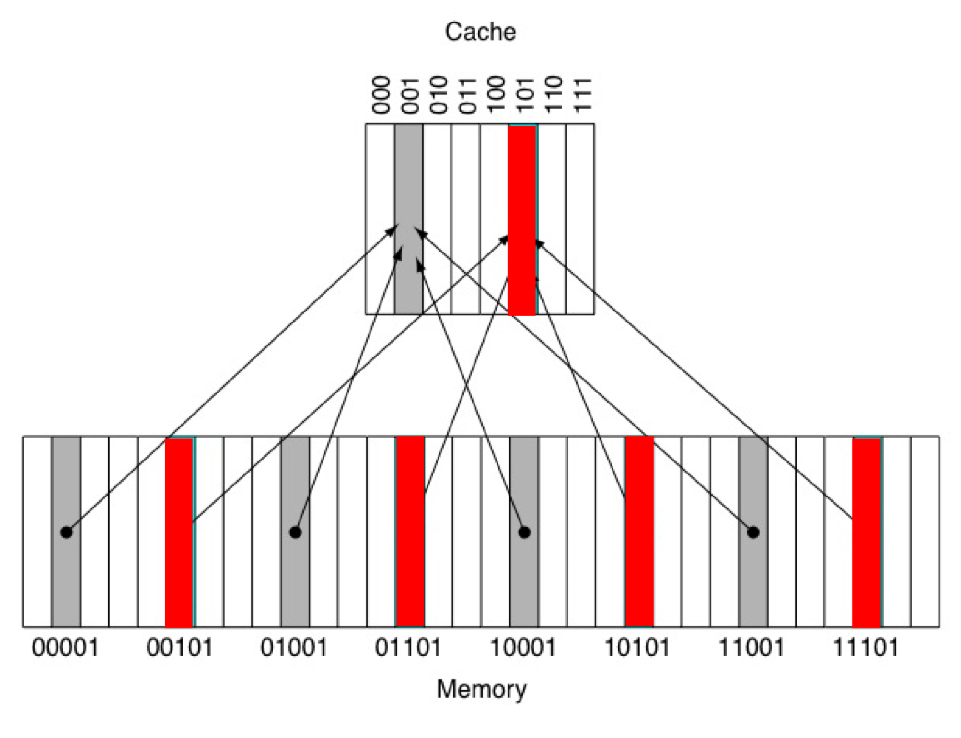
\includegraphics[width=80mm]{img/direct.png}
\caption{Direct Mapped Cache}
\end{figure}

\subsubsection*{Example}

For a direct mapped cache with eight 32-byte blocks, what is the index for a load with an effective address \texttt{0b0000 1000 0101 0100}?

---

The last $log_2(32) = 5$ bits are left for the block offset. So the block address is \texttt{0b0000 1000 010}. The index is therefore $$(\texttt{0b0000 1000 010}\ modulo\ \texttt{0b1000}) = \texttt{0b010}$$

In simpler terms, recall that we have 8 entries in the cache -- so we only need 3-bits to identify which entry in the cache. So identify the last 3-bits after we drop the 5-bits for the block offset, and that's our index.

--- 

\begin{figure}[ht!]
\centering
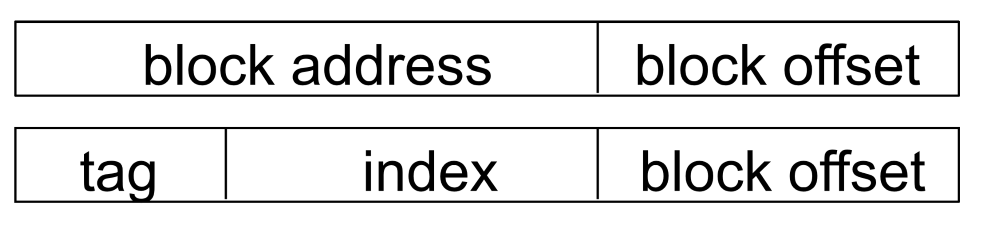
\includegraphics[width=60mm]{img/dmc.png}
\caption{Offset, Index, and Tag of a Direct Mapped Cache}
\end{figure}


Assume our cache is 1024 entries in 4-byte blocks, and this is our address memory address \texttt{0b1111 1010 0001 0000}.

The last $log_2(4) = 2$ bits are dedicated to the offset, so our offset is \texttt{00}. The next $log_2(1024) = 10$ bits are our index, so our index is \texttt{1010 0001 00}. The remaining bits are our tag, so our tag is \texttt{1111}.

Now let's look at how this is implemented in hardware. First we split the address into the offset, the index, and the tag. 

\begin{figure}[ht!]
\centering
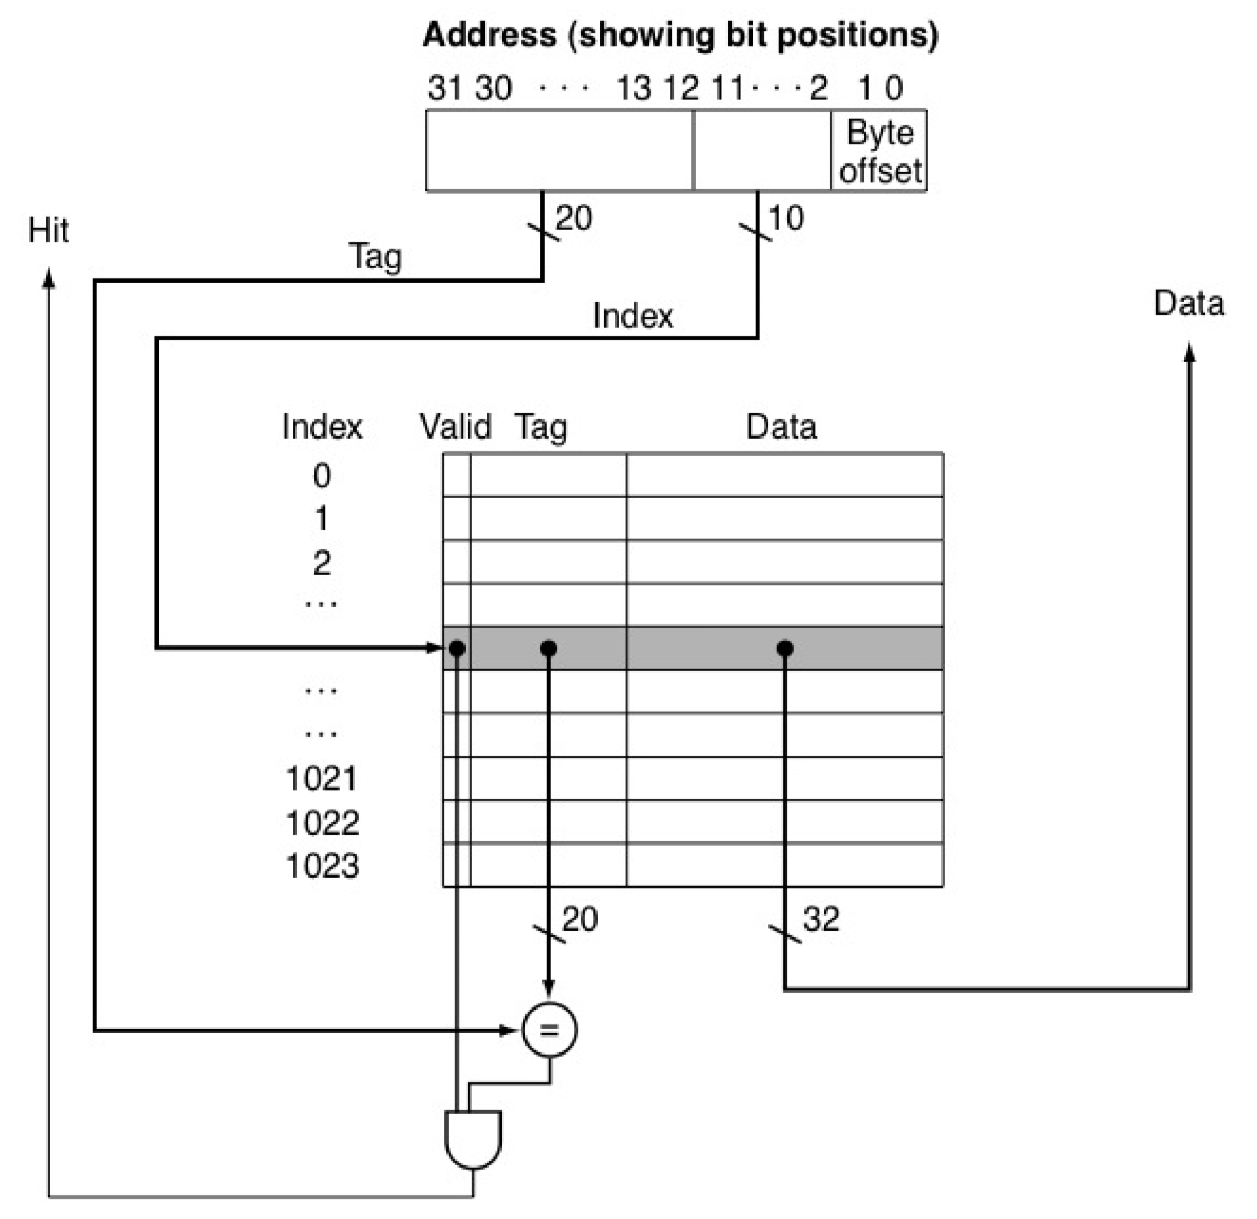
\includegraphics[width=100mm]{img/dmch.png}
\caption{Direct Mapped Cache Hardware Implementation}
\end{figure}

Then we use the index to locate the row in the cache. We read the tag and the data from that row. If the tag from the cache matches the tag from the address and the valid bit is set, we have a cache hit and so we raise the hit flag and retrieve the data.

A problem with the direct map cache is conflicts -- if we want to repeatedly access different addresses that map to the same row in the cache, then even if we have enough space in the cache to accommodate all the memory we want, because the cache is direct mapped we will continuously overwrite the data we want to keep in the cache.

\subsubsection{Set-Associative Cache}

In order to deal with conflicts, the set-associative cache combines some features of the fully-associative cache with some features of the direct-mapped cache.

The idea is that we will use the cache index to select a \textit{set} of blocks. In the direct-mapped cache we select one block, but here we select a set of 4-16 blocks. Then we treat this set of blocks like a small fully-associative cache. 

\begin{figure}[ht!]
\centering
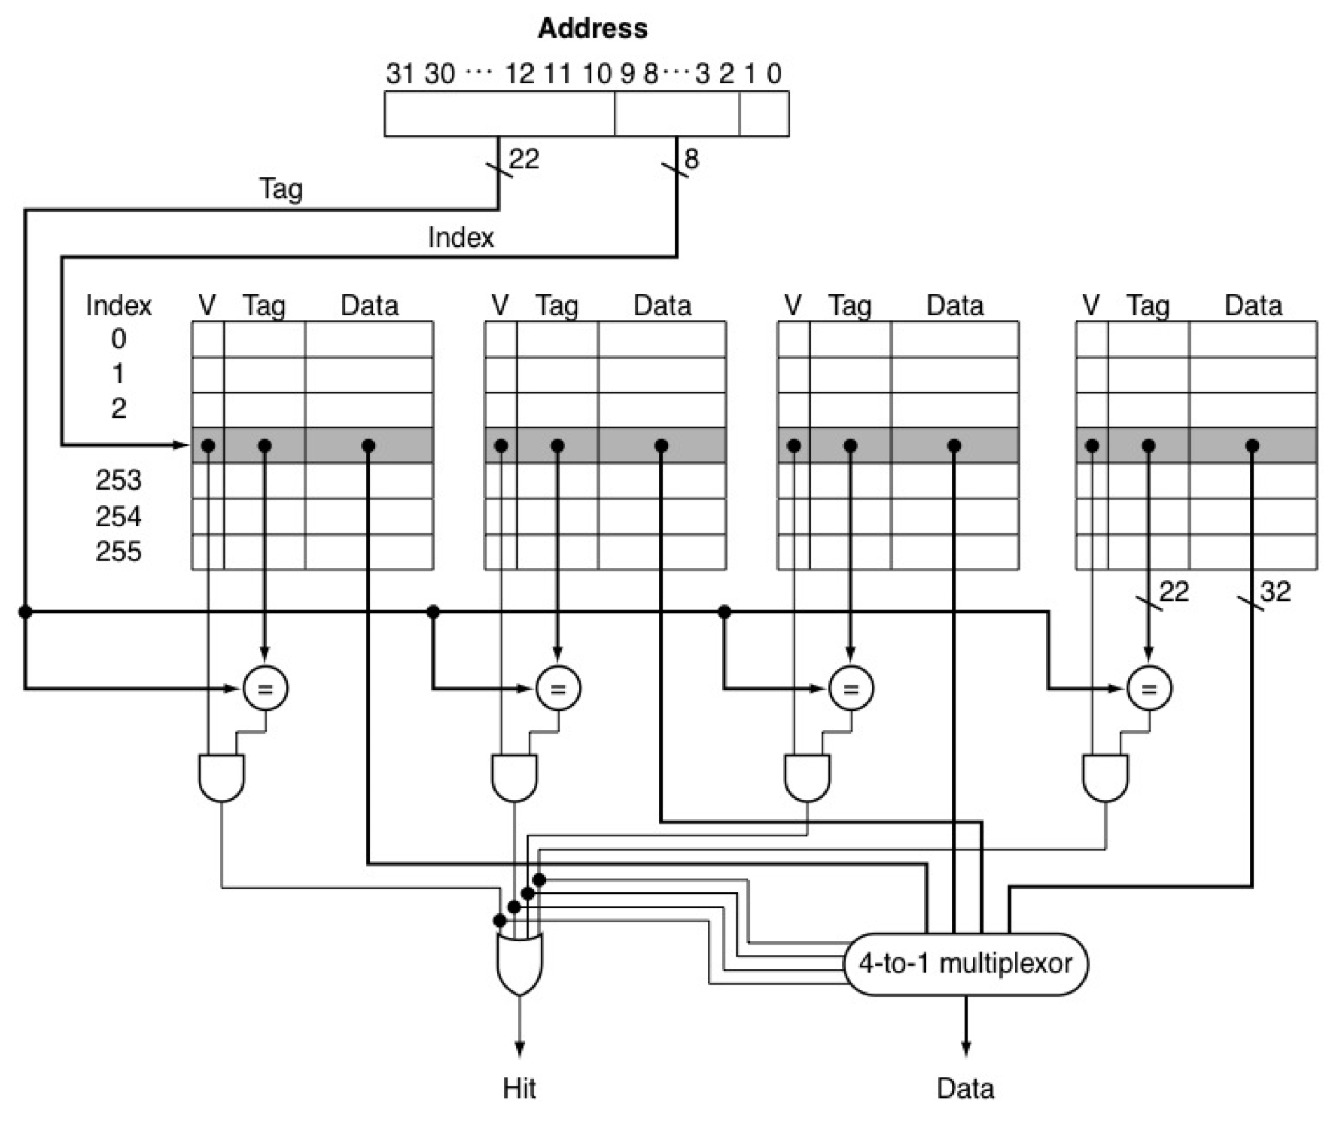
\includegraphics[width=110mm]{img/sac.png}
\caption{Set-Associative Cache}
\end{figure}

When the cache does a lookup, it indexes to the row of 4-16 different direct-mapped caches, creating a set of tags. Then we compare each tag in parallel to determine if any of them are a hit. If so, we will retrieve the data from the block with a matching tag using a mux. 

If there is a cache miss, we will only add them to empty entries. There will never be a situation in which two of the tables both return a hit.

Note that the number of ways does not need to be a power of two. It is independent of the index. 

\subsubsection*{Example}

How many sets (rows) is in a 4-way set associative cache containing a total of 32 16-byte blocks.

---

We 32 blocks and each block contains 16-bytes, and these are split between the four ways. 

So 32 blocks/4 = 8 blocks per way. The cache can have 8 sets. 


---

\subsubsection*{Example}

For a 4-way set associative cache containing a total of 32 16-byte blocks, what is the index for a load with effective address \texttt{0b0000 1000 0101 0100}?

---

There are $log_2(16) = 4$ bits reserved for the offset. So ignore those.

There are 32 blocks, but there are 4 ways, so there are 8 blocks per way. Thus there are $log_2(8) = 3$ bits required to index the 8 blocks. So the index is the bits \texttt{101}.


---

\subsubsection*{Example}

Let's say you're analyzing two potential designs for caches.

\begin{enumerate}
\item A direct-mapped cache with one-byte blocks and 8 bytes total

\item A 2-way set associative cache with 2-byte blocks and 16-bytes total
\end{enumerate}

The memory references are as follows 2, 3, 2, 8, 10, 2. Label the hits and the misses, and show the final cache contents. 

--- 

With option (1), there are 8 rows indexed by 3 bits. With option (2), there are four rows indexed by 2 bits, but each row holds two addresses. 

\begin{table}[H]
\scriptsize
\begin{tabular}{cc}
\toprule
\textbf{Set} & \textbf{Addr.} \\
\midrule
000 & \\
001 & \\
010 & 2 (miss) \\
011 & 3 (miss) \\
100 & \\
101 & \\
110 & \\
111 & \\
\toprule
\end{tabular}
\quad
\begin{tabular}{cc}
\toprule
\textbf{Set} & \textbf{Addr.} \\
\midrule
000 & 8 (miss) \\
001 & \\
010 & 2 (hit) \\
011 & 3 (miss) \\
100 & \\
101 & \\
110 & \\
111 & \\
\toprule
\end{tabular}
\quad
\begin{tabular}{cc}
\toprule
\textbf{Set} & \textbf{Addr.} \\
\midrule
000 & 8 (miss) \\
001 & \\
010 & 10 (miss) \\
011 & 3 (miss) \\
100 & \\
101 & \\
110 & \\
111 & \\
\toprule
\end{tabular}
\quad
\begin{tabular}{cc}
\toprule
\textbf{Set} & \textbf{Addr.} \\
\midrule
000 & 8 (miss) \\
001 & \\
010 & 2 (miss) \\
011 & 3 (miss) \\
100 & \\
101 & \\
110 & \\
111 & \\
\toprule
\end{tabular}
\end{table}

Both 10 (\texttt{0b1010}) and 2 (\texttt{0b0010}) are mapped to the same index location, so 2 is overwritten when the 10 is mapped. 


\begin{table}[H]
\centering
\scriptsize
\begin{tabular}{cl}
\toprule
\textbf{Set} & \textbf{Addr.} \\
\midrule
00 & \{\ ,\ \} \\
01 & \{[2 (miss), 3],\ \} \\
10 & \{\ ,\ \} \\
11 & \{\ ,\ \} \\
\toprule
\end{tabular}
\quad
\begin{tabular}{cl}
\toprule
\textbf{Set} & \textbf{Addr.} \\
\midrule
00 & \{\ ,\ \} \\
01 & \{[2 (miss), 3 (hit)],  \} \\
10 & \{\ ,\ \} \\
11 & \{\ ,\ \} \\
\toprule
\end{tabular}
\quad
\begin{tabular}{cl}
\toprule
\textbf{Set} & \textbf{Addr.} \\
\midrule
00 & \{[8 (miss), 9] ,\ \} \\
01 & \{[2 (hit), 3 (hit)],  \} \\
10 & \{\ ,\ \} \\
11 & \{\ ,\ \} \\
\toprule
\end{tabular}
\quad
\begin{tabular}{cl}
\toprule
\textbf{Set} & \textbf{Addr.} \\
\midrule
00 & \{[8 (miss), 9] ,\ \} \\
01 & \{[2 (hit), 3 (hit)],  [10(miss), 11] \} \\
10 & \{\ ,\ \} \\ 
11 & \{\ ,\ \} \\
\toprule
\end{tabular}
\quad
\end{table}

There are 2-byte blocks, so the lowest $log_2(2) = 1$ bit is used for the offset. And there are $16/2 = 8$ blocks per way, so $log_2(8) = 3$ bits are used for the index (???).

Since the blocks are 2-byte, we access 2 we also bring in address 3 into our block (and vice-versa). So 3 is a hit when we access 3. 

When we access 10, \texttt{0b1010}, we are mapped to \texttt{01}. Then we can put 10 and 11 into a free way. 

---


\subsubsection{Reuse Distance}

What do you do when the cache or set is full? Of course you need to replace things, but how do you decide what blocks to evict/replace?

If you remove the oldest data, you are taking advantage of temporal locality, but may not be taking advantage of spatial locality, and vice-versa. 

The optimal balance is the \textit{B\'{e}l\'{a}dy-optimal replacement} -- whereby you replace blocks re-referenced furthest in the future. The idea is that everything before that, you will need sooner, so it better be in the cache. 

However, the hardware does not know the future, so we need some prediction mechanism. We will do this using \textit{reuse distance}.

Consider the sequence of block accesses: \texttt{ABBCBCCDBBEDBBBA}. If you just look at A, there are 14 accesses between the two A accesses. In those 14 accesses, count how many unique blocks are accessed. In this case, there are four unique blocks, B, C, D and E. That means the reuse distance for A is 4.

\begin{equation}
Reused\ distance\ for\ X = \#\ unique\ blocks\ between\ accesses\ to\  X
\end{equation}
\myequations{Reuse distance}

But how do you know what reuse distance to optimize for? Through simulations of SPEC benchmarks, we can see that most references are to blocks with small reuse distances. Typically, recently used data is data that is accessed frequently, and thus has a short reuse distance. 

\begin{figure}[ht!]
\centering
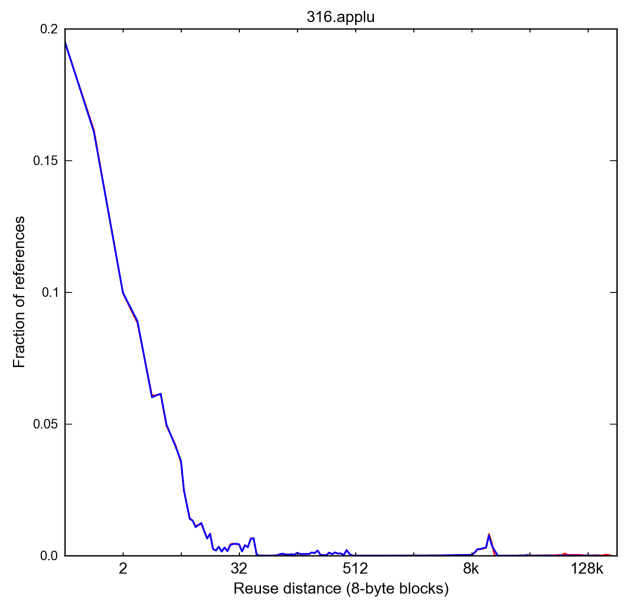
\includegraphics[width=80mm]{img/reuse.png}
\caption{Reuse Distance}
\end{figure}

\subsubsection{Replacement Policy}

This is how we will decide what blocks to evict. In general, you want to replace the least frequently used (LFU) data, or the least recently used (LRU) data. And actually random replacement works better than you would expect as well. 

To keep track of the LRU in a two-way associative cache, it would require one LRU bit. If you most recently accessed the data on the left channel, the LRU bit will point to the left (say a 0). If you most recently accessed the data on the right channel, the bit will point to the left (a 1). 

Then when you need to replace the data in a block, replace the block that the LRU bit is not pointing to. If the bit is 0, replace the right, otherwise replace the left.

If there are more than two ways, there are many choices for pseudo-LRU because perfect LRU is actually quite tricky. 

The most common and simple implementation is having one most-recently used (MRU) bit per block. Any time you use the block, set the bit to 1. Then once all bits have been set to 1, set all bits to 0 and restart the process. This isn't perfect, but it's pretty good.

A more sophisticated method is to have some kind of prediction number (reference prediction value) per block that is a prediction of when the block will be reference. When you insert a value into the cache or you have a hit, you set the value to maximum. Then over time you decrement the value over time. Every block's RRPV will decrement over time, but whenever you have a hit it will be refreshed to have a high value so it won't be replaced.

In each elbow of the following graph, that indicates that your array has exceeded the size of the cache and you start missing.

\begin{figure}[ht!]
\centering
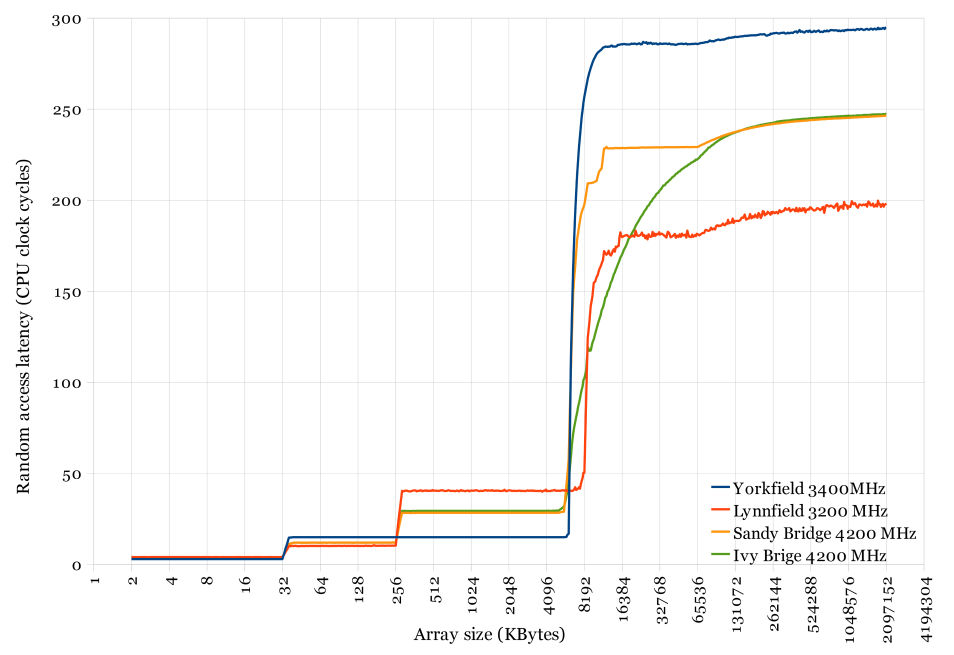
\includegraphics[width=100mm]{img/hits.png}
\caption{Latency of Difference Cache Levels}
\end{figure}

So each inflection indicates that you need to go to the next level cache to get your data, and each has more and more latency. Lower level caches use sophisticated replacement policies, and higher level caches don't. 

\subsubsection{Cache Misses}

There are three main kinds of misses.

\begin{enumerate}
\item \textbf{Cold start} (also called Compulsory) -- You will have cold start misses when your cache is empty or when you access a block for the first time. Increasing the cache size does not improve your performance for cold-start misses, the only thing that you can do is take advantage of spatial locality by increasing block size. 

\item \textbf{Capacity misses} -- This misses come from when your cache is not big enough. You used to have the value but needed to use that space for something else. If your cache was infinitely large, then you would never have capacity misses. 

\item \textbf{Conflict misses} -- These come from when you have a direct mapped cache and multiple things map to one entry. You would not have conflict misses if you had a fully associative cache. 
\end{enumerate}

Let's say you had a 2-byte directed mapped cache with 1-byte blocks. For the reference stream 0, 2, 2, 0 the second access to 0 misses. This miss will be a \textit{conflict} miss because both 0 and 2 map to the same one block. So the previously stored value from 0 has been replaced.

For the same cache, let's say you had the reference stream 0, 1, 2, and the access to 2 missed. This would be a cold start miss because it's the first time we access 2.

Again with the same cache, let's say the reference stream was 0, 1, 2, 0. The second access to 0 misses. This would be a capacity miss. 

\begin{figure}[H]
\centering
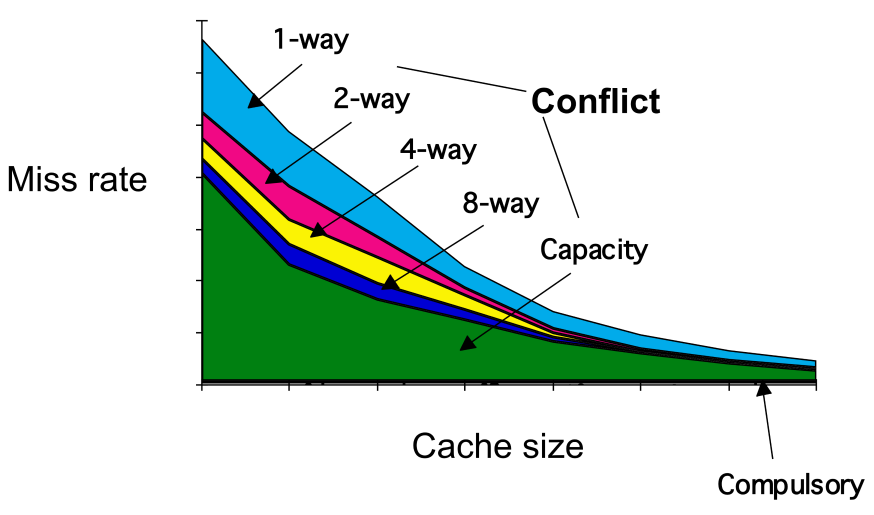
\includegraphics[width=100mm]{img/misses.png}
\caption{The Effect of Cache Size on the Miss Rate}
\end{figure}

You can see that as cache increases, the capacity miss rate goes down. You can also increase the number of ways which reduces conflict misses. In the end you're left mostly with mostly cold-start misses. 

However, if your cache block size increases too much, your miss rate will increase. Imagine your cache block size was the size of the entire cache, if it's too big then your cache is too dependent on spatial locality and will crowd out entries that take advantage of temporal locality. If your cache block size is too small however, then you will not be taken enough advantage of temporal locality. 


\begin{figure}[H]
\centering
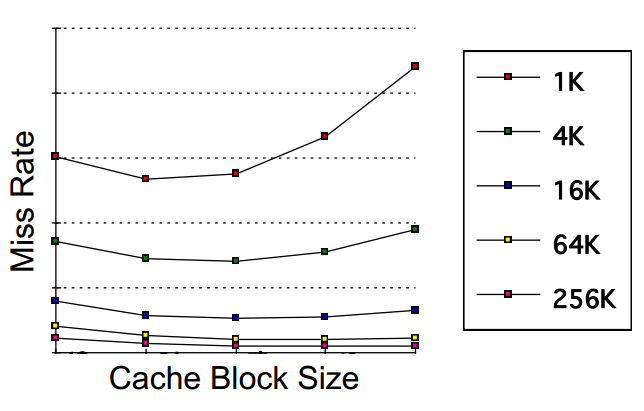
\includegraphics[width=80mm]{img/blocksize.png}
\caption{The Effect of Cache Block Size on the Miss Rate}
\end{figure}

As block size increases, you reduce the number of cold-start misses however.

\subsection{Cache Performance Impact}

In a simple in-order processor without a blocking cache, the CPU time is as follows. 

Miss-oriented approach to memory access. Here CPI includes both ALU and memory instructions.

\begin{equation}
CPUtime = IC \left(CPI + \frac{MemAccess}{Inst} \times MissRate \times MissPenalty \right) CycleTime
\end{equation}

If we separate out the memory component entirely, where AMAT is the Average Memory Access Time, and CPI only includes ALU operations. 


\begin{equation}
\begin{array}{rcl}
CPUtime & = & IC \left(\dfrac{AluOps}{Inst} CPI_{ALU} + \dfrac{MemAccess}{Inst} AMAT \right) CycleTime \\ 
\\
AMAT & = & HitTime + MissRate \times MissPenalty \\
\end{array}
\end{equation}

For aligned memory, there can be up to two cache misses on a single memory memory instruction. If memory is misaligned, there can be up to three misses. You must remember to take into account both instruction and data references to memory.

\subsubsection*{Example}

Assume CPI=1.0 when all memory references hit the cache, and assume simple in-order pipeline. The only data accesses are loads and stores and these are 50\% of the instructions. The miss-penalty is 25 clock cycles, the miss-rate is 2\%. How much faster is the CPU if the miss-rate is 0\%?

---

First compute the CPU time of a processor that always hits.

$$CPUtime = IC \times 1.0 \times CycleTime$$

Then compute the CPU time of a processor with a miss rate of 2\%. The CPI of ALU operations is 1. There are 1.5 memory accesses per instruction because each instruction takes one memory operation in the instruction fetch stage, and memory operations take another access and occur 50\% of the time.

\begin{equation}
\begin{array}{rcl}
CPUtime & = & IC \left(\dfrac{AluOps}{Inst} CPI_{ALU} + \dfrac{MemAccess}{Inst} AMAT \right) CycleTime  \\
\\
& = & IC \left( 1 + (1.5)(0.02)(25) \right) CycleTime \\ 
\\
& = & IC \left( 1.75 \right) CycleTime 
\end{array}
\end{equation}

So there is a 75\% speedup if there are always cache hits.

---

Upon store operations, there are different ways of updating memory. With the \textit{write-through} structure, both the cache and the main memory are updated from the CPU. With the \textit{write-back} structure, only the cache is updated, and main memory has invalid data. Main memory is only updated when the cache entry is about to be replaced.

Both of these strategies take use of a \textit{write buffer} to allow the cache to proceed as soon as the data are placed in the buffer. This means they do not have to wait all the time required for the update in main memory.

 With the \textit{write-evict} structure, the main memory is updated and the cache is cleared. 
 
How can we improve the performance of our cache?

\begin{enumerate}

\item \textbf{Larger block-sizes} in the cache  takes advantage of spatial locality and reduces the miss rate. This reduces compulsory misses but also increases the miss penalty. In smaller caches, block sizes that are too large can increase capacity or conflict misses, however. 

\item \textbf{Bigger caches} also reduce the miss rate. This reduces the capacity misses, but at the expense of longer hit times, more area, and more power consumption. 

\item \textbf{Greater associativity} reduces the number of conflict misses. Fully-associative caches have no conflict misses.

\item \textbf{Multi-level caches} reduce the miss penalty. You don't have to decide between small and fast caches or large and slow caches. 

\end{enumerate}


\clearpage
\section{Virtual Memory}

The main problem that virtual memory solves is that the operating system wants to multitask. It wants to run multiple programs simultaneously. If you have one processor that can run one thread, then your operating system can switch among multiple processes. 


It's convenient to assume that all programs assume that address space starts at 0. That way you can write your program one way where you assume where the program will be in memory, and you can run on any machine. 

Additionally, your computer may not have enough physical RAM to run all the programs at once. If you were running your operating system and your browser and your excel simultaneously, you would run out of physical memory and your PC would crash. 

Moreover these programs want a continuous range of addresses, not memory segmented into different chunks in different places in hardware. 


To solve this, we want each program to have a separate address space that begins at 0. We want to create the illusion for programmers and computer scientists that everything is normal and each program has its own \textit{address space ID} (ASID). So two programs executing simultaneously each thinks it has a separate copy of address 0 and address 1 and so one. These addresses are called \textit{virtual addresses} (VA).

As for real hardware memory, we will call these \textit{physical addresses} (PA). The CPU and the operating system will translate the VA to the PA. So programs with the same VA do not map to the same PA if they are in different ASIDs. 

We will split the memory into equal sized \textit{pages}, and we will keep a mapping between virtual pages and physical pages. 

\begin{figure}[ht!]
\centering
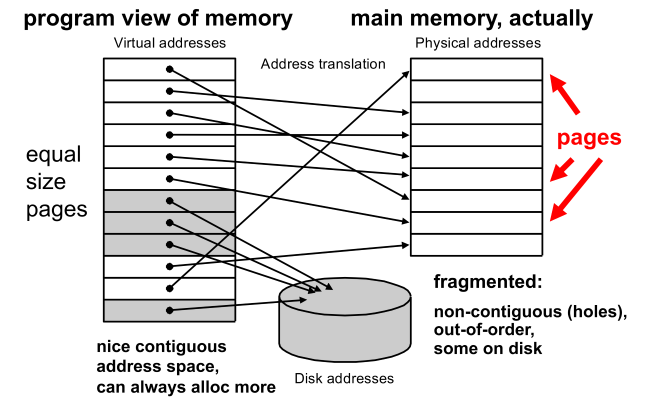
\includegraphics[width=90mm]{img/vm.png}
\caption{Virtual Memory Mapping}
\end{figure}

Even if physical memory is smaller than virtual memory, we can map virtual addresses to disk addresses. This means in the program view of memory, memory is continuous, starts at 0, and you can always allocate more. In reality, the memory is fragmented, so it is non-continuous, out-of-order, and some is on the disk.

To do this address translation, we will use a look-up table to determine the PA of VA. So we will have our virtual page number, which we translate to a physical page memory, but we don't change the page offset. If there are 12-bits for the page offset, then a page is $2^{12}$ = 4096 bytes = 4KB. 

First we need to have a register in the CPU that tells us where the look-up table is. And for each process that is running, we need a separate page table, so we will change this page table register.

\begin{figure}[ht!]
\centering
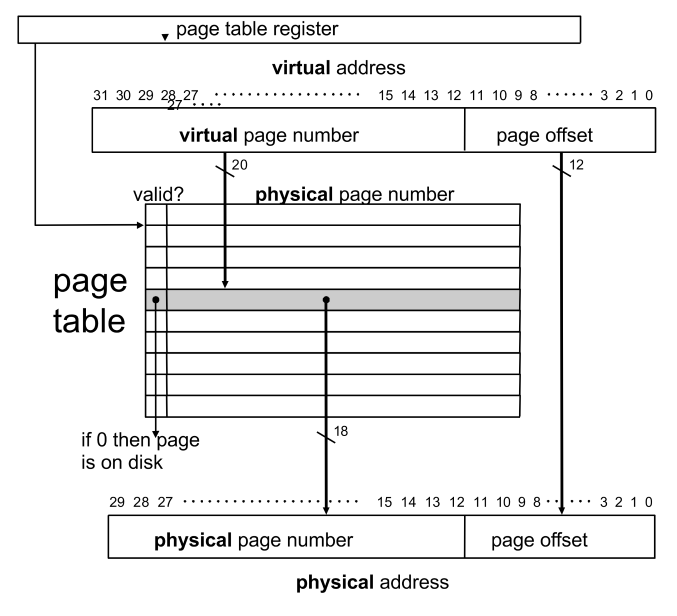
\includegraphics[width=100mm]{img/ptts.png}
\caption{Page Table Translation Structure}
\end{figure}

Note that the page table register holds a physical address because we need the page table to convert PA to VA. If the page table register was a VA, then we don't yet know how to translate it. 

If there are 30-bit physical addresses and 32-bit virtual addresses. The page offset is 12 bits, so we have 20 remaining bits for the physical address. So the page table is $2^{20}$ = 1048576 = 1M entries. 

An address translation is required not only for every data memory instruction, but for every instruction fetch since instructions are stored in memory. So for memory and load instructions, two address translations must be done.

We can't store these page tables near the CPU in a cache because they're just too big, but we also can't store them in main memory because doing translations every instruction would be unreasonably slow. 

\begin{figure}[ht!]
\centering
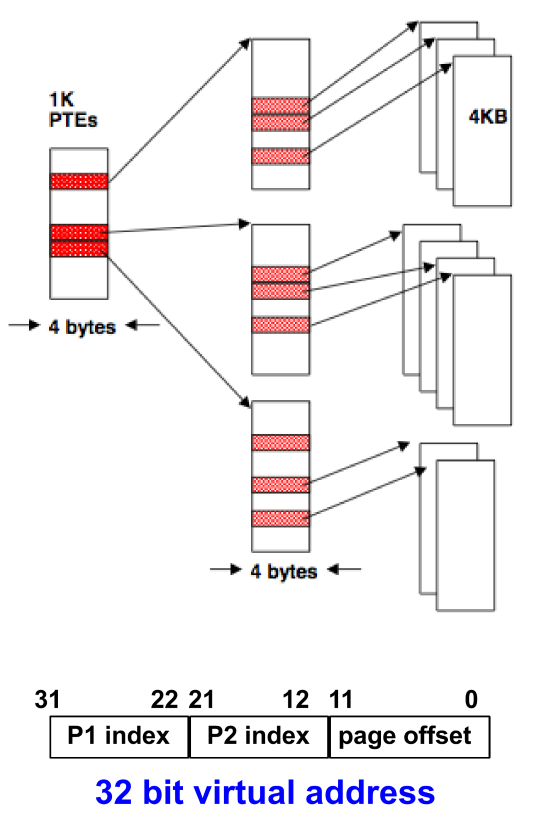
\includegraphics[width=60mm]{img/sparse.png}
\caption{Multi-level Page Tables}
\end{figure}

We know that each process needs its own page table because each process has its own address space. However, page tables are sparse. Most programs don't use all of their address space, so allocating an entire page table for every process is inefficient. So we create variable-size page tables and break them up into multiple levels.



The top-level table is in reserved in RAM. The next-level table can either be in RAM or in the disk based on the OS, and are not reserved, they are created and torn down as needed. 

This allows us to use much less memory total than if we had a page table for every process. 

So in our 32-bit virtual address, we break it up into two different indices and the page offset. The highest 10 bits represent the P1 index, the next 10 bits represent the P2 index, and the lowest 12 bits represent the page offset. 

These lower levels however are still stored in main memory, which is way too slow. So we will cache the page table in a \textit{translation lookaside buffer} (TLB). 

\begin{figure}[ht!]
\centering
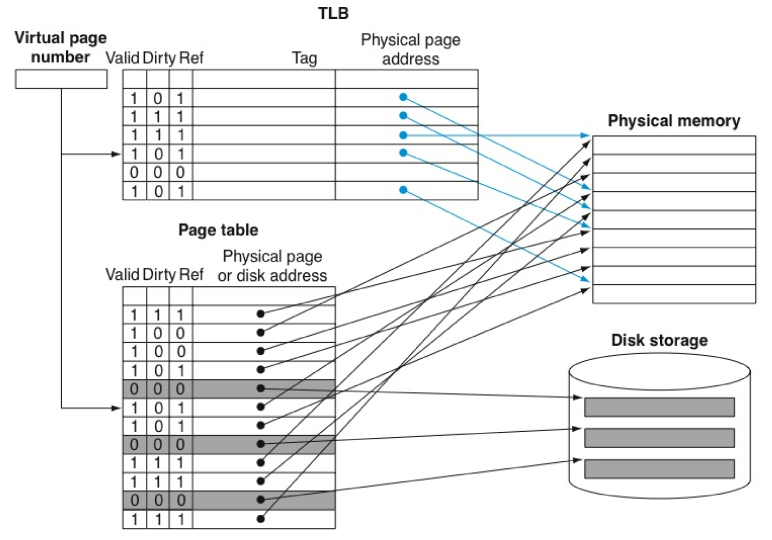
\includegraphics[width=110mm]{img/lookaside.png}
\caption{Multi-level Page Tables}
\end{figure}

The TLB is just a cache for the page table. The first level caches are fully-associative because it's less likely you'll have locality on a page-by-page level and it's fairly small. 

When we get a VA, first we check in the TLB, if the address is valid and we if we have a corresponding PA, then we can access the physical memory in one cycle. This way we don't have to access the page table in the RAM or the disk. 

If we have a miss, then we have to go to traverse the page table structure in memory, follow some pointers, and find the value. In x86 this is done in hardware, in MIPS it is done in software.

We also have to be concerned about rights. So if the page table is updated, the memory is updated, and vice-versa. We do this by using a "dirty" bit that indicates when a page table has been written. We can also include a read-only bit, in the event that multiple processes are running the same program and need to point at the same memory. If you write to it, you may interfere with the other process. You also may want an "execute" bit for security reasons, where you want to indicate some value is "data" and to never execute it so a buffer overflow hack can't get you to execute malicious code.


\begin{figure}[ht!]
\centering
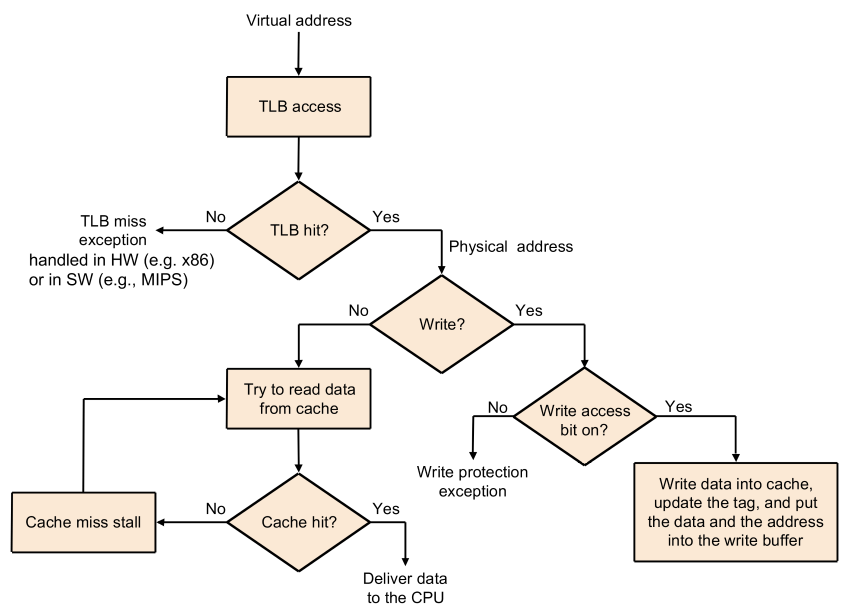
\includegraphics[width=110mm]{img/flow.png}
\caption{Memory Access Translation Flowchart}
\end{figure}

First you access the TLB. If you have a miss, you let the operating system figure out the exception. If you have a hit, then find the physical address.  If it's not a write read the data from the cache and check if you have a cache hit then get the data from the cache and we're done. If it's a miss then wait for the MSHR to tell us where the data is. If it's a write then update the tag, and it's not a write then throw an exception telling the operating system that someone is trying to write to protected memory.

We will translate the VA to the PA in parallel while you use the VA to access the data cache. Then use the PA to verify the tag is correct. 

If we have a virtually addressed cache and we switch from one process to another. Then we have to flush the cash because we would be looking at incorrectly translated VA to PAs. Flushing the cache takes up a substantial proportion of time, so instead of this we use ASID as well as the VA to address the data cache. 

If you want to share data across multiple programs however, then you'll include redundant data in the cache. 

Synonym problem (???). For each entry there are multiple possible entries in the cache. 

\section{Memory Technologies}

So far we have talked about keeping lots of data in lots of tables: the RF, caches, MSHRs, reservation stations, reorder buffer, branch predictor PHTs, branch target buffer, TLBs, write buffers,and so on. Almost everything requires keeping track on some data in a table.


\subsection{Random Access Addressing}

With RAM, you provide an address and the data is returned. There is no searching through the data like there is with associative lookup, rather you provide at tag and randomly access the data array. Caches use RAM, since you're not searching the data of the data table, you're providing a tag and getting the data at that tag. Predictably, RAM addressing uses technologies such as SRAM and DRAM (static and dynamic RAM). 

A memory table is seen in Figure \ref{fig:RAM}. Each cell in a memory array stores binary data. There are $2^{n-k}$ rows, and $2^{m+k}$ columns.  Provided an address of $n$ bits, \verb|addr[n-1:k]| select the row with the first $n-k$ bits, and \verb|addr[k-1:0]| selects the word with the latter $k$ bits.

What's $m$ (???)

\begin{figure}[ht!]
\centering
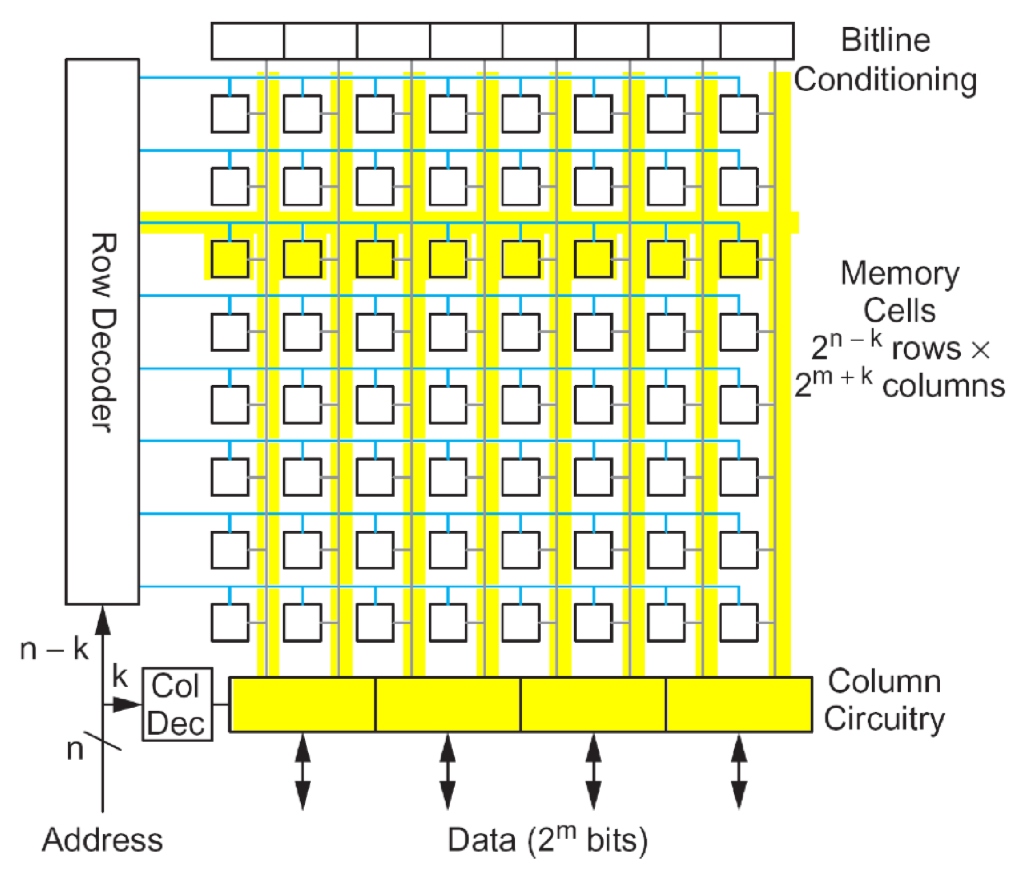
\includegraphics[width=80mm]{img/RAM.png}
\caption{RAM Data Array}
\label{fig:RAM}
\end{figure}

For speed, you want the array to be roughly square, where $n \approx m$. Wires have to span all the way up and down and right and left, and the longer the wire the more capacitive it is, which adds latency. The horizontal rows are the \textit{wordlines} and the vertical rows are the \textit{bitlines}. 

To perform a read operation, you use the address to index a row and drive each cell on a row. This opens each cell and forces the cells to drive their respective bitlines. 

These cells are very small in order to make memory dense, which means they cannot drive strong signals on the long bitlines. So the bitlines are preconditioned somehow (different for SRAM and DRAM) and the cells either pull up or pull down the bitline, which is then amplified to a strong 0 or 1 with sense amplifiers.

To perform a write operation, again the wordline is indexed and driven by the address from the row decoder, which then opens up the cells on that row. Then the value to be stored drives the bitlines. Since the bitlines can be driven by a powerful signal and the cells are weak, the values stored in the cell are overpowered and the cells retain the data. 

\subsubsection{SRAM}

In SRAM, each bit is stored with an SRAM cell -- essentially a back-to-back inverter. This is a positive feedback loop as each inverter reinforces the value of the other inverter, so there is no leakage. These two inverters cost four transistors, plus two "access" transistors which we use to load and read values.

\begin{figure}[ht!]
\centering
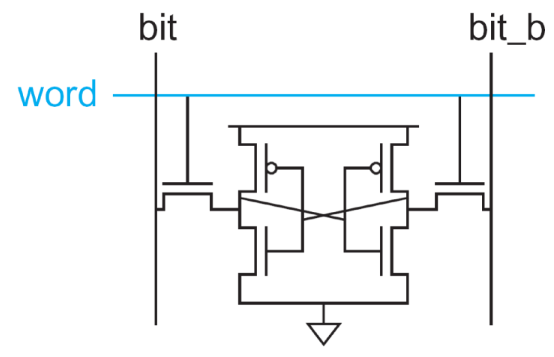
\includegraphics[width=50mm]{img/SRAM.png}
\caption{SRAM Cell}
\end{figure}

As we said, to read a value from the SRAM cell, we precharge both the \verb|bit| and \verb|bit_b| (as in \textit{bit bar}, the inverse) lines to high. Then we turn the wordline high to enable the access transistors ("enable the cell"). This will then ground one of the bitlines, which will tell us the value in the SRAM cell.

To write, we set the bitline to the value we want to store (and the inverse bitline to the opposite). One of the lines will then be high, and this will overpower the logic in the cross-coupled inverters and save the value.

\begin{figure}[ht!]
\centering
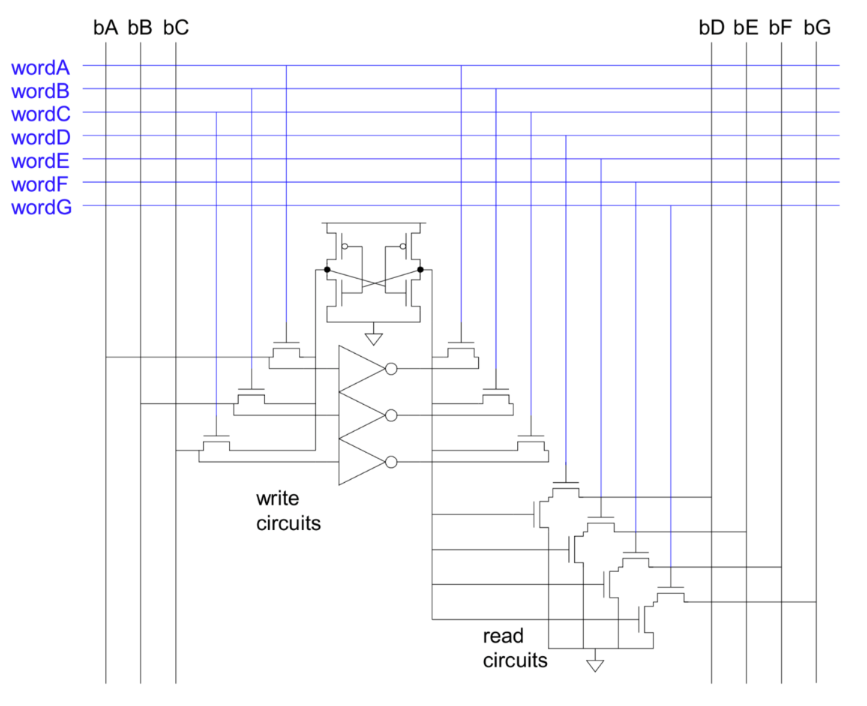
\includegraphics[width=80mm]{img/Multiport.png}
\caption{Multiport SRAM Cell}
\end{figure}

However, you may want to read or write to different sets of bits (words) on the wordline separately. However, with this SRAM cell, you only have one port so you cannot individually index words on the wordline. For instance, in the MIPS architecture, when reading instructions you may need to read two different operands from the register file in one cycle. Or you may want to read and write different words in the same cycle. To do this, we need multi-ported SRAM cells.

If you want to take this further and simultaneously read and write from a cell, you cannot use this from the above cells. Consider this example register file cell, it has separate read and write lines. This means that if we read and write from the same cell in one cycle, the value will just be forwarded from the writeline to the readline. 

\begin{figure}[ht!]
\centering
\includegraphics[width=60mm]{img/RF.png}
\caption{RF Cell}
\end{figure}

\subsubsection{DRAM}

A DRAM cell is just one capacitor and transistor. It is very small so it is very dense and cheap. Since the capacitor is so small, it is very weak and cannot pull a bitline fully up or fully down, so we precharge the bitline to $V_{dd}/2$, so when the DRAM cell is opened up, it only slightly drags down the voltage or slightly bumps it up. This slight disturbance is then amplified to be a zero or a one.



When we read a value from a DRAM cell it is called destructive because we lose the former value of the DRAM cell, so we must write-back values we read. The capacitor also leaks and loses charge over time, so we must occasionally refresh the DRAM cells by reading and writing back the values. Currently they are refreshed around once every 64ms. 


\begin{figure}[ht!]
\centering
\includegraphics[width=80mm]{img/DRAM.png}
\caption{DRAM Cell}
\end{figure}

This is not manufactured using the same logic as typical CMOS. The transistor must be strong enough to drive a large bitline, but weak enough that it can be overwritten easily, so it is bigger than logic transistors.

To do our refresh or to write-back the value after we read it, we use a register called the row buffer. We read the array and store it in the row buffer, then send the data where it needs to go from the row buffer. 

The row buffer can be thought of as a tiny cache. If we immediately get another request to DRAM for the same address, then we already have the value in the row buffer so this is called a row buffer hit, and we can immediately pass the value along without reading from the DRAM. 

However if we get another request for a different address it is a miss, then we use the row-buffer to write the values back into the last DRAM row and then get the new value requested. We wait before writing back to avoid any potential unnecessary writes when there are hits. Before the row-buffer writes back the values, the row is said to be "open", after it has written them back it is said to be "closed". 




\subsection{Associative Lookup Addressing}

As an alternative to RAM, whereby you provide an address and get the data at that address. But associative lookup means you provide a key and are told whether the key is in the memory. Fully associative means you have to look through the entire cache. For instance TLBs are small fully-associative caches. These use a technology called Content Associative Memory (CAM). 

\subsubsection{CAM}

Similarly to SRAM, the storage unit is cross-coupled inverters. Below, we have a match line, which means we use 10 transistors for each CAM cell. The purpose of the match line is to learn whether the value driven on the bitlines is the same as the value stored in the cells. 


\begin{figure}[ht!]
\centering
\includegraphics[width=50mm]{img/CAM.png}
\caption{CAM Cell}
\end{figure}


To do this, we precharge the bitlines and the matchline to high. Then we drive the key on the bitlines, if the value in the cell is not equal to the value driven on the bitline, then the matchline will be shorted to ground. If not, then the matchline will stay high. 

To write to the CAM cell, it is the same as an SRAM cell, we charge the bitlines to the value, then set the wordlines to high and it will overpower the cross-coupled inverters. 

\begin{figure}[ht!]
\centering
\includegraphics[width=60mm]{img/CAMs.png}
\caption{CAM Structure}
\end{figure}


If we expand the CAM cell out to an entire CAM structure, we get a situation where any mismatch of a cell and bitline in a row can set the row's matchline to zero. Only rows will exact matches will have a high matchline. These matchlines can then be sent to an OR gate which will tell us if there exists a match in memory.

Reservation station, TLB, branch target buffer, and load-store queue, can all use some sort of CAM because they look for some sort of match. 

\section{Memory Consistency}

With multi-core processors, we must communicate between the cores using shared memory. If core 0 writes to a shared memory location and core 1 reads from that location, we need to ensure that the process in core 0 has completed first. You don't want to read data in a half-written state or incorrect data needed for dependencies.

To order accesses to shared memory, we can use flags. Consider the code in the two threads in Figure \ref{Flag}. Thread B cannot continue until Thread A has set the flag, which will only occur after the data has been set to the updated value. 

\begin{figure}[ht!]
\centering
\includegraphics[width=110mm]{img/flags.png}
\caption{Flags between threads}
\label{Flag}
\end{figure}

This flag effectively communicates that thread A has finished storing the data and it is safe for thread B to load it. These restrictions are needed in both multi-cores and single-cores with multiple concurrent threads.

Memory access reordering happens in the compiler, inside the CPU core such as with store buffer or load-store queue, in the interconnect between cores/chips. It also can happen in DRAM, when there are reads of the address that is already stored in the row buffer, they may be prioritized over reads to other addresses because the data is already available and will take overall less time to give that first. 

The point of this is that memory access reordering happens very often, and we can find ourselves in trouble without a model to determine what reording is acceptable. 

\subsection{Memory Consistency Model}

A memory consistency model specifies what sequences of memory states are permissible. If there are multiple cores looking at the memory, the memory consistency model sets the rules for what different cores are allowed to see and modify what values of memory. To do this, each memory is given a state to keep track of what operations are allowable on it.

It also tells us which memory accesses are allowed to be reordered. This is due to the above states, for instance if one core is not permitted to read or write to a certain value, then it is clear there is some sort of dependency and reordering is not allowed, s it must wait until that state changes. 

\subsubsection{Sequential Consistency (SC)}

A processor is sequentially consistent if the result of any execution is the same as if the operations were operated in some sequential order. There doesn't have to be a specific sequential order, there can be many valid sequential orders, but it just needs to be consistent with one of those orders. (???) More importantly, the operations of each processor must appear in order specified in that processors program.

The instructions of each processor can be interleaved with each other in any order, but the order of operations must be in the program order in each individual processor. 

Let's say core 0 needed to execute instructions \verb|A B C D| and core 1 needed to execute instructions \verb|1 2 3 4|, then the following would be SC execution: \verb|ABCD1234|, \verb|A1B2C3D4|, \verb|AB12CD34|, \verb|1234ABCD|.  However, \verb|ADBC1234| is not sequentially consistent because the order of one individual processor was not in program order. 


\subsubsection*{Example}

Consider the following program orders in each core, where initially X and Y have a value of 0.

\begin{verbatim}
Core A                  Core B
A1: store X <- 1        B1: store Y <- 1
A2: load r1 <- Y        B2: load r2 <- X 
\end{verbatim}

Assuming a SC system, what are the possible values of r1 and r2 after both threads have finished? For all possible outcomes, what are the SC orderings.

---

\begin{verbatim}
Order          r1  r2
A1 A2 B1 B2    0   1
A1 B1 A2 B2    1   1
B1 A1 B2 A2    1   1
B1 B2 A1 A2    1   0
\end{verbatim}


However, the outcome could never be r1=0 and r2=0 because a store must always happen before a load.

---

Recall we spent some time discussing optimization with the store buffer or the load-store queue which provide us with something like 20-25\% performance improvement. The store buffer allows loads to bypass stores because there aren't memory dependencies. However, this only checks for memory dependencies within one core. 

If we revisit the above example but include a store-buffer that moves a load before a store, then we can get the result r1=0 and r2=0, which is \textit{not} sequentially consistent.

To maintain SC, for all memory accesses within each core we have to maintain:

\begin{enumerate}

\item \textbf{Load-to-load ordering} -- If we swap two loads, then we will lose sequential consistency. For instance, consider the thread B in Figure \ref{Flag}, the load of the flag must happen before the load of the data. 

\item \textbf{Load-to-store ordering} 

\item \textbf{Store-to-store ordering} 

\item \textbf{Store-to-load ordering} -- It doesn't matter if there is not a direct data dependency in the core, we cannot bypass loads because there may be a transitive dependency in another core.
\end{enumerate}

However, this is inconvenient for performance purposes beacuse we lose the performance boosts we got from reordering with the store-buffer. The main cause of this issue however is the interleaving nature  of the cores. 

\subsection{Weak Ordering (WO)}

If we ensure that all the memory writes in one core are completed before the memory reads in the second core start, then we avoid these logical constraints. Then we can still allow reordering in the individual cores as allowable by the store-buffer, and not have to worry about dependency problems between the cores.


We will implement this by allowing arbitrary reordering \textit{except} for synchronization operations. We will put a synchronization operation at the end of the writes in core 0, and put a synchronization operation at the beginning of the reads in core 1. 

Recall our previous example. Here, the flag operations are our synchronization operations.

\begin{figure}[ht!]
\centering
\includegraphics[width=110mm]{img/flags.png}
\caption{Flags between threads}
\label{Flag2}
\end{figure}

Within the cores, the operations can be reordered however they want. To implement WO we must ensure the following rules.

\begin{enumerate}
\item Finish all prior loads/stores before the synchronization operation

\item Finish all prior synchronization operations before executing loads/stores

\item Ensure synchronization operations are sequentially consistent
\end{enumerate}

Typically, these synchronization operations are implemented in hardware with \textit{memory fences}. These operations do not actually do a read or a write, they just indicate that everything before a fence must finish before anything after the fence can start.


\begin{figure}[ht!]
\centering
\includegraphics[width=110mm]{img/fence.png}
\caption{Fence operations}
\end{figure}

 Additionally, no operations can be reordered across a fence to ensure fences are synchronously consistent.

\subsection{Release Consistency (RC)} 
 
 Fences could also be considered too strong of a constraint. The main concern between dependencies across different cores is one core, let's call it core 0, finishing all of its writes before the other core, core 1, begins its reads. 
 
 It is not actually a concern if loads in core 0 after the fence leak before the fence, or if stores in core 1 before the fence leak after the fence as long as there are not actual data dependencies. 
 
 To implement this we will break fences out into two categories. One fence will ensure stores go before the fence, and one fence will ensure loads go after the fence. 
 
 \begin{figure}[ht!]
\centering
\includegraphics[width=110mm]{img/release.png}
\caption{Release consistency fence operations}
\end{figure}
 
 Think of this as a lock. If you want to write a whole bunch of things to a data structure, you acquire the lock, finish your writes, then release your lock.
 
 \begin{enumerate}
 \item \textbf{Release} -- all prior loads/stores must be completed before release store
 
 \item \textbf{Acquire} -- all acquire loads must be completed before any subsequent loads/stores start
 \end{enumerate}
 
 This allows optimization like the store-buffer and LSQ because you can allow loads to bypass stores and still keep this model. 
 
 In summary: Loads and stores after the release can be executed before the release. Loads and stores before the acquire can be executed after the acquire. 

 
 \begin{figure}[ht!]
\centering
\includegraphics[width=120mm]{img/reorderingdiagrams.png}
\caption{SC, WO, and RC reordering diagrams}
\end{figure}
 
\subsection{Total Store Ordering (TSO)}

Most performance increases come from relaxing the store-to-load ordering -- that which says loads cannot bypass stores. TSO, which is implemented in x86, keeps load-to-load, load-to-store, and store-to-store ordering, but allows stores to be reordered after loads.

\subsection{Store Atomicity}

So far our examples have just been fences between two processors. We require fences to operate on a global-scope. If one processor is waiting for a value to be set by another processor, then gets the updated value, \textit{store atomicity} means that all other processors also get the updated value. 
 \begin{figure}[ht!]
\centering
\includegraphics[width=110mm]{img/store.png}
\caption{Store Atomicity}
\label{Atom}
\end{figure}
 
Without store atomicity, we can get broken causality. For instance, observe Figure \ref{Atom}, without store atomicity, $P_3$ may not get the updated value of $A$ and could illogically print 0.

\section{Coherence}

Caches in multicores add another factor to the problem of consistency because multiple copies of a memory block can exist in the system. If memory is updated in one cache or in memory, how do we know that the cache of other cores is not providing that core with an out of date value. Our previously discussed consistency models do not address this.

Let's say core 0 does a load of memory address X, then core 1 does a load of memory address X. Then both cores have a copy of X in their cache. If core 0 then writes a value to address X its cache will be updated, but core 1 will have an incorrect value in its cache. 

Moreover, if both cores write a different value to address X, which value is written back to shared memory? This depends on which cache must evict the value first.

For a system to be coherent, we must break out memory accesses into read-only and write epochs. The \textit{Single Writer Multiple Readers (SWMR) Invariant} states that if there are multiple copies of a cache block, they must be read-only because if copy is changed the other copies will be incorrect. If there is a writable copy of a cache block, it must be the only copy.

\subsection{Modified, Shared, Invalid (MSI) Protocol}

The objective of the coherence protocol is to maintain the SWMR invariance.
We implement this with the MSI protocol, which assigns each memory block a state.  The state indicates the permissions of the block. 

\begin{enumerate}
\item \textbf{Modified} -- The block may be read or written. According to SWMR invariance, there may only be one copy of memory in M state. 

\item \textbf{Shared} -- The block may be read but not written. According to SWMR invariance, there may be multiple S copies.

\item \textbf{Invalid} -- The block may not be read or written, it is a useless block.

\end{enumerate}

Each processor's cache is connected to shared memory and each other through a common bus. To simplify, for now now we will assume communication on this bus is instantaneous. 


 \begin{figure}[ht!]
\centering
\includegraphics[width=60mm]{img/cachecontrol.png}
\caption{Cache Controller}
\end{figure}

Each cache will also get a local cache controller to update the states of the memory blocks. When there are loads/stores from the core, the cache controller must update the state of the block and issue coherence requests on the bus. Other caches will listen on the bus and see these coherence requests and update their own cache's states accordingly.

\begin{table}[ht!]
\small
\begin{tabular}{cll}
\toprule
\textbf{State} & \textbf{Memory Sees} & \textbf{Cache Sees} \\
\midrule
M & One cache has a dirty copy & Block  cached with write permissions \\
S & Multiple caches have clean copies & Block cached with read-only permissions \\

I & No cache has a copy & Block is not cached \\
\toprule
\end{tabular}
\caption{MSI Protocol States}
\end{table}

\begin{enumerate}
\item \textbf{Read hit} -- If the value requested is in the cache in S or M state, then we do not need to send any bus messages because no one has a modified copy and we will not write to the value

\item \textbf{Read miss} -- If the value to read is not in the cache, then the block is in the I state. So we must send a message on the bus to request the block. 

If another cache has the block in the M state, it must downgrade it to the S state in order for there to be multiple copies and send us the latest value. 

\item \textbf{Write hit} -- If the block is in the M state then it is the only copy and we have permission to write to it. 

Since we are the only block with a copy, then we don't have to write and bus messages.


\item \textbf{Write miss} -- We have a write miss when the block is either in the S state or the I state in our cache. 

If the block is in the I state, we must send a write-request on the bus. If another cache has the block in the M state, it will invalidate the block because it will soon be outdated, and sends us the latest value.

If the block is in the S state, we must send an invalidate request on the bus so that other caches send their copy to I so we can change our copy to M. We do not need to be send a copy because we already have the latest value.

\end{enumerate}

All the state transitions together are reperesented in the state machine in Figure \ref{MSI}.


 \begin{figure}[ht!]
\centering
\includegraphics[width=80mm]{img/MSI.png}
\caption{MSI Protocol State Machine}
\label{MSI}
\end{figure}

\begin{table}
\centering
\begin{tabular}{ccc}
\toprule
\textbf{Initial} & \textbf{Situation} & \textbf{Final} \\
\midrule
I & CPU wants to read & S \\
I & CPU wants to write & M \\
S & CPU wants to write & M \\
M & CPU has write-miss then gets updated value & M \\
S & CPU has read-miss then gets updated value & S \\
M & CPU has read-miss then gets updated value & S \\
M & Bus has read-miss (ie. someone else wants to read the block) & S \\
S & Bus has write-miss (ie. someone wants to write to the block) & I \\
M & Bus has write-miss & I \\
\toprule

\end{tabular}
\end{table}

\subsection{Directories}

Previously we assumed that messages can be transmitted immediately on the bus. However, this is not true. The number of cores on CPUs or GPUs can be very high. For instance on the Intel Xeon Phi there are 72 x86 cores. For these types of processors, the buses would have to go between all cores and so the buses would have high capacitance and would be too slow. 

To get around this, we will use multi-cycle interconnects, such as a ring or mesh or torus. This means that the transmission of messages will take multiple cycles to move from one core to another core, and we have unpredictable latency. This prevents us from being able to listen on the bus. Instead we will send all messages to one place called a directory. This directory can be split physically but logically it is one entity. 

The directory will provide the similar functionality to the previously described bus. The directory will know all sharers who have a copy of a given block, and the state of each block. Usually the directory is attached to a piece of memory. 

It differs from the bus in that we must track each state explicitly. In the bus protocol each memory block in cache had a state, but here we also track the state of blocks in main memory.

Each entry in the directory contains the following
\begin{enumerate}
\item \textbf{Presence bitvertor} -- Indicates which cores contain copies of a block. One bit is reserved for every core in the system and if the bit is high then it contains a given cache block.

\item \textbf{Dirty bit} -- Indicates if a block is in the M state43
\end{enumerate}

\subsubsection{Directory MSI Protocol}


The cache and the directory communication with the directory protocol. This protocol consists of three kinds of places. 

\begin{enumerate}
\item \textbf{Local node} -- This is the originating cache, ie. that of the processor making a request.

\item \textbf{Home node} -- This is where the directory entry is stored.

\item \textbf{Remote node} -- This is a cache that contains a copy of the data we are interested in.
\end{enumerate}

Let's suppose we make a load request. Then the local node sends a message to the hom node requesting to get permissions to turn to an S state to read. 

The home node may know there is another copy of the block in another cache, in which case the home node must send a message to the remote node requesting that it downgrade its state from M to S. We don't know how many cycles it will take for message to reach the node and return a confirmation. 

Once the home node gets confirmation, it sends a message to the local node granting it permission to turn to an S state. 

We will have two controllers, one will be located at the cache and one will be located at the directory. These controllers will have to communicate with one another. 

\section{VLIW and SIMD}

So we've seen a few different architectures that can be classified by Flynn's taxonomy. The most straightforward classification is where one instruction is associated with a single piece of data. 

You could also consider situation where multiple instructions perform an operation on a single piece of data. This is an uncommon architecture, but perhaps an example could be where one funtional unit performs an approximation very quickly, and another functional unit calculates the exact result but takes more time, then these values can be compared later. Video encoding could use an architecture like this. 

After that you can consider multiple instructions performing operations on multiple  pieces of data in parallel. An example of this would be a multicore processor. 

 \begin{figure}[ht!]
\centering
\includegraphics[width=80mm]{img/flynn.png}
\caption{Flynn's Taxonomy}
\end{figure}

Finally, the architecture we will be talking about in this section, is that where a single instruction is performed using multiple pieces of data. Examples of this could be dot products or matrix multiplication. GPUs have this structure, whereby a whole bunch of threads are glued into one instruction. This is called the Single Instruction Multiple Data domain (SIMD). 

Let's back up and look at what we have covered so far. We have used out-of-order superscalar cores to run a sequence of instructions, and these use one thread of execution at a time. 

When we compile our code, we remove any parallelism that we may know ahead of time by creating just sequence of instructions. Any parallelism that we know ahead of time isn't told to the hardware. We have just used very clever tricks like register renaming, reservation stations, and the reorder buffer to extract as much parallelism as possible during execution. An then we have dealt with control flows that limit how much parallelism we can do, and so implemented  speculative execution to squeeze some more performance out of these processors. 

But by doing this, we've ended up devoting most of our hardware and most of our transistors to managing the execution, not actually performing computations. The amount of area on the processor that makes up the ALUs is minute in comparison. And this just seems inefficient, so let's look at some alternative  solutions. 

\subsection{Very Long Instruction Word (VLIW)}

The main point here is that a lot of the parallelism that the processor is extracting for you during run time, we already actually know at compile time.

Let's say we see a for loop like the following.

\begin{verbatim}
    int N = 100;
    for(int i = 0; i < N; i++)
    {
        vect1[i] = someComputation(i);    
    }
\end{verbatim}

At compile time, we can see that these  \texttt{N} computations  can be performed in parallel. However the compiler may incorrectly turn this into a sequence, or worst-still make us evaluate the branch every time. 

So instead of this we're going to write in our code specifying where the independent operations are so the processor isn't trying to figure it out on the fly. To do this, we'll make one large instruction with a bunch of operations and tell the hardware that all the pieces of this big instruction can be executed in parallel, and it doesn't have to worry about the sequence or the dependencies. 

 \begin{figure}[ht!]
\centering
\includegraphics[width=100mm]{img/vliw.png}
\caption{VLIW}
\end{figure}

This spares us doing all this dynamic scheduling and the processor doing a whole bunch of work to make sure that it can actually perform these operations in parallel. These are very common in for example data-signal processors. To create these VLWI, we can do a few things at compile time. 

\subsubsection{Loop Unrolling}

This resolves some parallelism limitations imposed by branches. Let's look at an example. In the following code, basically what happens is that the value at each value in an array is incremented \texttt{f2}. 

\scriptsize
\begin{verbatim}
loop:
l.d    f0, 0(r1)    
daddi  r1, r1, #-8  
add.d  f4, f0, f2    
s.d    f4, 8(r1)    ; mem[r1] = mem[r1] + f2 ; r1 -= 8;
bnez   r1, loop     ; if(r1!=0) loop
\end{verbatim}
\normalsize

So let's say we don't want to devote much silicon to implementing a good branch predictor. In that case we can unroll this loop four times. By doing this, we only have to do one immediate addition calculation and one branch evaluation every equivalent of four loops. 


\scriptsize
\begin{verbatim}
loop:
l.d   f0, 0(r1)
add.d f4, f0, f2
s.d   f4, 0(r1)   ; drop daddi & bne

l.d   f0, -8(r1)
add.d f4, f0, f2
s.d   f4, -8(r1)  ; drop daddi & bne

l.d   f0, -16(r1)
add.d f4, f0, f2
s.d   f4, -16(r1) ; drop daddi & bne

l.d   f0, -24(r1)
add.d f4, f0, f2
s.d   f4, -24(r1)

daddi r1, r1, #-32 ; alter to -4*8
bne   r1, r2, loop
\end{verbatim}

\normalsize
Of course in this example, it requires that the array be a multiple of four. So typically there would be some cleanup code that checked for that. 

The other problem limiting our parallelism is our dependencies and conflicts from reusing our registers. 


\subsubsection{Register Renaming}

This resolves the limitations to parallelism imposed by limited registers. 

In the above unrolled code we must wait for one block of \texttt{l.d}, \texttt{add.d}, and \texttt{s.d} to complete before beginning the next because we reuse the registers \texttt{f0} and \texttt{f4}. 

If we rename the subsequent registers, then each section can be executed in parallel. 

\scriptsize
\begin{verbatim}
loop:
l.d   f0, 0(r1)
add.d f4, f0, f2
s.d   f4, 0(r1)

l.d   f6, -8(r1)
add.d f8, f6, f2
s.d   f8, -8(r1)

l.d   f10, -16(r1)
add.d f12, f10, f2
s.d   f12, -16(r1)

l.d   f14, -24(r1)
add.d f16, f14, f2
s.d   f16, -24(r1)

daddi r1, r1, #-32
bne   r1, r2, loop
\end{verbatim}
\normalsize

This requires the compiler to know how many registers we have and that we have many registers. 

\subsubsection{Software Pipelining/Instruction Reorder}

Real data dependencies can also cause stalls, which limits our parallelism. We can overcome some of this by reordering instructions. 

Again, in the above unrolled code we must wait until \texttt{f0} has been loaded before doing our addition, and we must wait until our addition has been done before storing \texttt{f4} into memory. 

However, instead of stalling between each of these operations, we can observe that each loop is independent and by reordering all the loads first, then all the additions second, then all the stores last, we do not have any stalls due to data dependencies. 

But perhaps we will still have stalls due to structural hazards due to the loads/stores. To resolve some of this, a compiler would do memory address analysis to prove different operations don't alias the same memory location, in which case it's okay to put them in parallel. 

\scriptsize
\begin{verbatim}
loop:
l.d   f0,  0(r1)
l.d   f6,  -8(r1)
l.d   f10, -16(r1)
l.d   f14, -24(r1)

add.d f4,  f0,  f2
add.d f8,  f6,  f2
add.d f12, f10, f2
add.d f16, f14, f2

s.d   f4,  0(r1)
s.d   f8,  -8(r1)
s.d   f12, -16(r1)
s.d   f16, -24(r1)

daddi r1, r1, #-32
bne   r1, r2, loop
\end{verbatim}
\normalsize

The other assumption we're making here is that if we reorder these accesses it won't violate our memory consistency model. In reality we may need to ensure sequential consistency, or we could reorder but would need to implement fences for a weak-ordered or release-consistent model to indicate where we have dependencies.

\subsubsection{Limitations}

In order to maximize efficiency, we must schedule so that the most functional units are all operating in parallel. 

 \begin{figure}[ht!]
\centering
\includegraphics[width=120mm]{img/vliw2.png}
\caption{VLIW Scheduling}
\end{figure}

This requires a very clever compiler. Tasks such as pointer aliasing are notoriously difficult. 

To compile effectively, we must know the number of cycles the operations take, and in the case of memory operations the latency is unpredictable due to cache misses/hits. We could also have branch mispredictions. This is one of the limitations of a compiler driven approach and is why high-performance processors still use out-of-order superscalar. 

We also have to encode things like the number registers and instruction latencies in our code. This creates a problem with binary compatibility, because different architectures or even different versions can have different latencies or hardware. So the code would need to be recompiled to run on these different architectures. 

But still, by doing all of these optimizations at compile time, we have saved ourselves having to implement a ROB or RSs, a Tomasulo register-renamer, and a fancy branch predictor in silicon. We also don't have to waste hardware by tracking dependencies because intra-instruction operations are guaranteed to be independent.

\subsection{SIMD Instruction Encoding}

Recall the code discussed in the previous section was the operation of adding a scalar to a vector. This is a very common operation in video/audio, 3D graphics, DNNs, scientific simulations, etc. 

\scriptsize
\begin{verbatim}
loop:
l.d    f0, 0(r1)    
daddi  r1, r1, #-8  
add.d  f4, f0, f2    
s.d    f4, 8(r1)   
bnez   r1, loop     
\end{verbatim}
\normalsize

So instead of using a loop that the processor may or may not know has dependencies, let's just create a separate instruction for it. 

\scriptsize
\begin{verbatim}
ldv    v0, 0(r1)    ; load vector
addvs  v4, v0, f2   ; add vector and scalar
sv     v4, 0(r1)    ; store vector
\end{verbatim}
\normalsize

This way the processor knosw ahead of time from the encoding that each iteration is independent. And the single instruction can be dispatched to multiple FUs in parallel. The compiler recognizes loops that can be assembled as vector operations rather than branches in the assembly. This can be implemented in hardware in two ways.

\subsubsection{Spatial SIMD -- Array Processor}

These computations can be distributed spatially, like multicores. Here we send each pair of operations to a separate functional unit. 

 \begin{figure}[ht!]
\centering
\includegraphics[width=100mm]{img/simds.png}
\caption{Spatial SIMD}
\end{figure}

\subsubsection{Temporal SIMD -- Vector Processor}

We can also distribute the computations across time, basically take the vectors and compute them with deep and fast pipelines that do not need to check for any dependencies. 

 \begin{figure}[ht!]
\centering
\includegraphics[width=30mm]{img/simdt.png}
\caption{Temporal SIMD}
\end{figure}

There is some startup cost due to loading the vectors, but the longer the vector the more this startup cost can be made up for. 

In reality, most SIMD architectures use both spatial and temporal SIMD. 

\subsubsection{Problems with SIMD}


\begin{enumerate}
\item \textbf{Short vectors} -- Some vectors are smaller than the amount of space we allocate for our vectors. 

So we use a Vector Length Register, VLR, so that when loops are unrolled they're not unrolled to 64 iterations when the vector is only 3 elements. In CPUs mostly they use fixed leng vectors. 

\item \textbf{Long Vectors} -- Data has more elements than we have vector registers. We can solve this using strip mining. 

\item \textbf{Per-element conditional operations} -- Consider a for loop with an if statement inside of it. The compiler may want to assemble the loop as a vector operation, but the if statement throws a wrench in the works. 

\scriptsize
\begin{verbatim}
for(i = 0; i < 64; i++)
   if(X[i] != 0) 
      X[i] = X[i] - Y[i] 
\end{verbatim}
\normalsize 

We solve this using a a mask that will write to the array only if the mask is set. 

\item \textbf{Non-contiguous vectors} -- If vectors are scattered in memory. Solved using stride. 

\item \textbf{Sparse vectors/matrices} -- Stride might not be constant, so use scatter/gather accesses. 

\item \textbf{Big RAW penalties} -- If there are vector operations that have dependencies, these can cause long stalls. We get around this using chaining, which forwards each element as it is computed. 

\item \textbf{Memory bandwidth} -- Vectors can be spread across many rows in RAM, and RAM can only read one row at a time, taking many cycles to read a vector. The soluction is to  vectors across multiple banks in the same row , so they can all be read simultaneously. 
\end{enumerate}

\section{GPUs}

GPUs are general purpose multicore processors. They're basically SIMD machines with some added clever scheduling to run independent threads. 

A core is effectively a unit that can issue instructions. A GPU has about 6-60 cores, which are called streaming multiprocessors (SMs)\footnote{Industry has different terminology for different companies. For instance what NVIDIA calls "warps", AMD calls "wavefronts". For consistency, we'll stick to using the NVIDIA terminology.}. They have thousands of functional units, which for marketing purposes are called CUDA "cores", even though they're not really cores.

GPUs, unlikey CPUs, are optimized for throughput. CPUs are optimized for latency, they have a single thread of instructions that are optimized for extracting parallelism and optimizing this single thread as fast as possible. With GPUs, they don't care about executing each instruction individually really fast, for instance drawing each pixel really fast. Rather, you care about drawing the whole image really fast.

CPUs have lots of overhead, devoted to management of these instructions. GPUs have SIMD hardware, whereby each core (SM) has warps which are 32-64 wide vector elements that can be operated on. 

We also want the GPU to be able to do some out-of-order execution so we also have an in-order scoreboard. We don't have a ROB through. In GPUs we don't care if instructions are executed (and committed) out of order. The reason we didn't want to do this in CPUs was because if there were interrupts or incorrect speculation, and we needed to be able to handle them and reset to the previous state. In GPUs we don't handle interrupts and don't execute anything speculatively. 


 \begin{figure}[ht!]
\centering
\includegraphics[width=100mm]{img/CPUvsGPU.png}
\caption{GPU vs. GPU Area}
\end{figure}

This saves us lots of control overhead. No speculative execution, no instruction reordering, no branch prediction. So instead we can dedicate the area to doing the execution. The in-order scoreboard and cache don't take much area equivalently.

GPUs also have huge register files. A GPU can have upwards of about 32,000 registers, whereas a typical CPU might have 100. And the DRAM of GPUs has a higher bandwidth. 


Basically what GPUs have to do is convert millions of vertices, a bunch of triangles in memory, into millions of pixels. These many computations -- calculating the colour, lighting each vertex, etc. --  are independent. This parallelism can be made explicit to the GPU, whereas a CPU assumes that all the instructions are sequential. 

Recall than a single VLIW is actually a packet of independent instructions. This long instruction is fed simultaneously to many different functional units and the GPU knows they can be executed in parallel. 

 \begin{figure}[ht!]
\centering
\includegraphics[width=90mm]{img/VLIW3.png}
\caption{VLIW}
\end{figure}

This contrasts with vector processing/SIMD, whereby we add vector registers and extra instructions and see that a single instruction can be spread across multiple independent FUs. 

 \begin{figure}[ht!]
\centering
\includegraphics[width=90mm]{img/SIMD3.png}
\caption{SIMD}
\end{figure}

However, vector processing requires rewriting programs to use these instructions or using a very sophisticated compiler. We also need to rewrite our program again if our hardware vector width changes. 

The other challenge with this concerns the programmer, because it's very hard to visualize and write programs doing computations on every single vertex simultaneously. It makes sense to execute instructions this way, but we don't want to program this way. It's easier to express our computations \textit{per} vertex, or \textit{per} pixel. This is called SIMT, for single-instruction multiple threads. 

 \begin{figure}[ht!]
\centering
\includegraphics[width=90mm]{img/SIMT.png}
\caption{SIMT}
\end{figure}

Here we're not programming a vector, rather we're programming multiple threads and in the background it is executing a single instruction in lockstep. 

Let's look at an example in terms of programming. This is what a adding a constant scalar to a vector would look like in vector programming:

\scriptsize
\begin{verbatim}
addconst(base, len, c) {
   set_vlr(len);
   vector_load(tmp, base);
   vector_add(tmp, tmp, c);
   vector_store(base, tmp);
}

addconst(base, len, 42);
\end{verbatim}
\normalsize 

With a SIMT program, we only are concerned with one thread at a time. Here we have a variable called \texttt{tid} for the thread ID. This way thread 1 will read the first element, thread 2 read the second element, and so on. And we can run \texttt{addconst} at every thread. We can also use this to specify single elements in a vector.

\scriptsize
\begin{verbatim}
addconst(base, len, c) {
   if(tid <= len){
   	   tmp = *(base+tid);
   	   tmp += c;
   	   *(base+tid) = tmp;
   }
}

addconst<65536>(base, len, 42);
\end{verbatim}
\normalsize 

In the first example, the vector operations show the instructions can be executed in parallel. With the second example, the function itself looks sequential. The parallelism is expressed through the \texttt{<65536>}, which shows the function will be invoked on 65536 different threads. Each thread will execute the same instruction but on different data, accessed using the thread id \texttt{tid}. This allows us to execute a SIMT program, which is easier to write, on SIMD hardware.

These threads will be bundled together into one SIMD instruction. 

If there are two indices where the \texttt{<65536>} is, these indentify the \texttt{<\# blocks, \# threads>}. We'll be talking about a single core/SM, so we'll focus on different threads, but one blocks runs on one SM, so these can also index cores.

\subsection{Warps}

Given let's say 64 threads, we'll break these threads chunks of 16, called warps. All threads in a warp will be running the same SIMD instruction so they have the same PC, and all threads will run in lockstep.

 \begin{figure}[ht!]
\centering
\includegraphics[width=90mm]{img/warps.png}
\caption{Warps}
\end{figure}

Lots of the data has a very different access pattern than that of a CPU. With a GPU you grab a triangle from memory, do some computation on it, and put it back it to memory. After that you're never expected to see the triangle again. This is called a streaming access pattern and has very little temporal locality, which changes our cache design for GPUs.


While latency isn't that important, throughput is very important. To maximize throughput we need to keep all our functional units busy. To do this, we're going to use lots of warps in our GPU and run each warp independently. The GPU can then schedule these warps in whatever order it wants. 

We're going to multiplex these warps in time. So if one warp is stalled due to a cache miss, then we can switch to run another warp. Since these warps are independent, this isn't a problem. In order to cover latencies of a cache miss, we need between 32-64 warps. 

So in summary, first we decided to take a bunch of threads, squish them together, and treat it like one vector instruction. Second we decided to use fine-grain multithreading to multiplex these warps to cover individually long latencies and maximize throughput. 

Because each thread is running indpendently, then each thread needs to have its own private storage. So each thread gets its own registers. 

 \begin{figure}[ht!]
\centering
\includegraphics[width=70mm]{img/warpreg.png}
\caption{Warp Registers}
\end{figure}

When all threads in the warp are executing the same instruction they will be using the same register references, so they need their own register sets. 

This looks a lot like SIMD architecture. There is one instruction for each warp, and it is operating on vector registers. It is doing some sort of vector operation, then writing these back to a vector register. 


\subsection{Challenges}

Instruction fetch for fine-grain multithreading is quite complicated, but want to keep our rate of issuing at 1 or more instructions per cycle. If we overcome this complexity, we can take advantage of the fact that we can amortize latency. 

Diverting branches within a single warp is also quite complicated. Each thread can compute an address from its thread ID, but also we can use this thread ID like so \texttt{if(tid\%2)==0} to get different behaviour from different threads. 

We also have a giant register file. In a modern GPU this can be around 256KB, compared to our MIPS64 architecture which was about 256B. This can require 4 accesses per instruction to our register file. We can achieve this by adding multiple read/write ports, but this costs about 2x the amount of area, making the RF even larger. 


\subsection{Architecture}

We have multiple SIMT cores, each of which has huge register files. They have interconnect networks to connect to a last-level cache (usually L2) and have high-bandwidth memory that is specialized for graphics. Ultimately this architecture resembles that of a CPU multicore. The main difference between a high performance  GPU and that in your phone is just the number of cores.

 \begin{figure}[ht!]
\centering
\includegraphics[width=80mm]{img/GPU.png}
\caption{Generic GPU Architecture}
\end{figure}

Let's zoom in to within the core. We have a SIMD data path which is a bunch of deeply pipelined functional units which we can feed vectors into. We also have a large register file, our caches (L1, texture, constants, and shared memory -- a scratchpad).  We also have the SIMT front end which allows us to fetch instructions for multiple warps, schedule which warp to run at a given time, and deal with branches. 


 \begin{figure}[ht!]
\centering
\includegraphics[width=80mm]{img/gpucore.png}
\caption{Generic GPU Core Elements}
\end{figure}

Zooming in even further, let's look at the path of instructions through the SIMT and SIMD. First we decide what instruction to fetch, then get it from the instruction cache, then we decode the instruction. Once we decode it we can put it in the instruction buffer and the in-order scoreboard. Then we figure out what warp to issue, so we get the registers from the operand collector and then do the operating by accessing memory or the ALU. After this you can writeback to update the register file and the scoreboard. 

 \begin{figure}[ht!]
\centering
\includegraphics[width=100mm]{img/gpucore2.png}
\caption{Inside an NVidia-style GPU Core}
\end{figure}

We have three schedulers -- fetch, issue, and execute. One schedules which instruction to fetch from the instruction cache. The second is the warp scheduler, which with the in-order scoreboard decides which warp to use next. The third is the operand collector, which is a very large banked register file. 

\subsubsection{Fetch and Decode}

In the fetch and decode stages, the only difference between a GPU and a CPU in this stage is that each warp has a different PC. Here we arbitrate the instruction cache among multiple warps. 

If you have a cache miss or a longer-latency operation, then skip it while its stalled and fetch other warps to cover the latency.

Once we have the instruction we decode it and put it in the instruction buffer. The instruction buffer holds the instruction with a valid bit to tell us if it has all its operands and is ready to be executed. 

We use an in-order scoreboard to track which registers are being written to and which registers are being expected by each instruction to take care of hazards. 

We don't really care about completing out of order because as long as the frame completes we synchronize after we complete. We don't need an out-of-order scoreboard because in a GPU because we can cover latency by switching to execute other warps -- we're not trying to cover latency by extracting parallelism from independent subsequent instructions. It also saves us using extra hardware.

\subsubsection{Instruction Issue}

The second scheduler is the warp scheduler, which selects a warp that is ready from the scoreboard and chooses the next warp to execute. Then it issues the next instruction in that warp.  There are two common schedulers. 

\begin{enumerate}
\item \textbf{Loose-Round-Robin (LRR)} which issues instruction from the same warp until it stalls, then chooses the next warp in the cycle. \item \textbf{Greedy-Then-Oldest (GTO)} which issues from the same warp for as long as possible in order to not overwrite data in the cache that's relevant to that warp (taking advantage of locality). When it runs out of instructions in that warp, it chooses the warp that is the oldest to complete. 

\end{enumerate}

Recent GPUs are superscalar -- they can issue multiple warps per cycle. 

They also  have a replay mechanism to avoid stalling in the pipeline. What this means is that when an instruction is issued from the instruction buffer, it is kept there until the instruction is complete. 

Imagine a scenerio where there is a load-miss. We send the load to the execution unit, the execution unit accesses the memory. Instead of waiting for the load to return a value, the GPU will forgot about this instruction and issue something else then reissue this instruction later when the load has returned a value. We can do this because we don't care about the relative order of warps. 

\subsubsection{Branch Divergence}

We still want to keep our SIMD architecture whereby we deploy the same instructions to all threads, but we may want different threads to execute different code.

We can use a vector mask, \texttt{VMASK}, which computes some condition for each thread (element of the vector) and we will skip threads for which \texttt{VMASK[i]==0}.  These instructions predicated on some condition, so they are called predicated instructions.

\scriptsize
\begin{verbatim}
addconst(base, len, c) {
   if (tid % 2 == 0) {     // condition acts as VMASK
      if (tid % 3 == 0) {
        ...
      } else {
        ...
      }
   }
}
\end{verbatim}
\normalsize

The main challenge here is that there can be nested branches. If there are two branches then we need two separate vector-mask registers. But this code can become confusing as we try to specify specific branches. This becomes very challenging when writing functions, especially nested functions because they're not sure what \texttt{VMASK} to use.

 \begin{figure}[ht!]
\centering
\includegraphics[width=50mm]{img/reconvg.png}
\caption{Reconvergence Stack}
\end{figure}

So what we do is hold these \texttt{VMASK} on a stack. The current execution path forms a stack, and at some point all branches reconverge eventually. We can combine these ideas to form a SIMT Reconvergence Stack. 

This stack holds three pieces of data.

\begin{enumerate}
\item \textbf{Reconvergence PC} -- This has the PC of where we reconverge, and if there is nothing here then we are not in a branch

\item \textbf{Next PC} -- The following instruction's PC

\item \textbf{Active Mask} -- This tells us which of the threads are going to be executed on this branch 
\end{enumerate}

Using this, when we encounter threads that go different ways, we execute one thread along a certain path of branches, then start again at the beginning and execute the other threads that went another path. 


We know when we have finished a given path when we hit the reconvergence PC that it stored in the stack.

\subsubsection{GPU Register Files}

Recall that these are very big. MIPS64 has 32 64-bit registers, so a 256 byte register file. In comparison, the NVidia Pascal has 64 warps, each with 32 threads, each with 32 32-bit registers, so a 256 KB register file.

We also must access four registers per instructions: one to write to, and three to read from (for multiply-and-add $ab+c$). We don't use multiports because they are too expensive in terms of area (every additional port is $2\times$ the area). 

So instead of one 4-ported register file, we will have four 1-ported register file banks. Each of these banks can be accessed independently. Recall these are vector registers, so we  have one wide register per warp not one register per thread. 

We want to minimize the number of conflicts, so we can place our faith in the compiler to allocate in such a way to avoid conflicts. But consider the following code:

 \begin{figure}[ht!]
\centering
\includegraphics[width=50mm]{img/banks.png}

\scriptsize

\begin{verbatim}
                mad r2, r5, r4, r6
                add r5, r5, r1 
\end{verbatim}
\normalsize

\end{figure}

For the \texttt{add} instruction, both of Warp 0's \texttt{r5} and \texttt{r1} are in Bank 1. Since these banks are single-ported, it can't read both of these operands at once. Moreover, it's the same problem with Warp 1, which is also trying to read these operands. So this instruction wants to read four  registers from bank 1 and also write to two registers, which means we need to stall a lot. 

We can solve the second problem, the overlap between Warp 1 and Warp 0, issue somewhat by hashing the warp ID as part of the register file layout. 

We will try to avoid the first problem's bank conflicts using the operand collector described in the next section.

\subsubsection{Operand Collector}

The idea behind this is to mix up accesses to the register file from multiple warps in the same cycle to avoid bank conflicts.

To do this, we need a structure to hold an instruction and track when the operands of an instruction are ready from the register file, then send it to execute. We call this the operand collector, but it's very similar to the reservation stations described with CPUs. 

This allows the RF to read from multiple warps in the same cycle. This gives us a longer pipeline because of these reservation stations reducing our latency, but improving our throughput. 

\subsubsection{Scalar Registers and Execution Units}

A lot of the time we don't need to do vector-vector operations, we need to do vector-scalar operations. Using an entire vector to do an operation with a constant wastes time, energy, and space. So we can also include a scalar unit to execute one instruction (not a vector instruction) for the whole warp.  

\subsubsection{GPU Memory Systems}

DRAM is special for GPUs because we need higher bandwidth for all the data we're running through the GPU. We're also always reading and writing at once, so we keep two rows open at once instead of one. We also use some compressing to save bandwidth for pixels that have the same colours and we can just average.

Also to improve throughput, memory accesses are coalesced. This means that from a single warp you will be accessing blocks on the same cache-line to reduce the number of accesses to the cache, similar in principle to an MSHR. 

Cache blocks are also about twice as large in GPUs as in CPUs. We can get away with this because there is very little temporal locality in GPUs. These caches also tend to be write-through or write-evict to prefer streaming cache accesses. 

We also have a scratchpad (caches keep copies of data, scratchpads aren't copies, they're the only data), a texture cache, and a constant cache. We also have an L2 cache, which is the last-level cache (LLC). On a CPU the LLC would more likely be a L3 or L4 cache. 

When we rasterize the vertices, we do this in a grid called mipmaps containing differing levels of detail. The texture cache is organized such that we can write data into blocks that take advantage of geometric locality. 

%--------------------------------%







\newpage
\bibliography{references}
\bibliographystyle{apacite} 
\pagebreak


% -------- APPENDIX -------- %
\appendix
\onehalfspacing
\section*{Appendix}
\addcontentsline{toc}{section}{Appendix}
\renewcommand{\thesubsection}{\Alph{subsection}}

\subsection{Tutorial 1}

\subsubsection{Amdahl's Law}

\paragraph{Assuming 80\% of a program could be parallelized perfectly (executing on N cores, speedup is N). If
you have a 32-core computer, what's the speedup you could get compared with the single core machine?
If you have infinite number of cores, what's the maximum speedup?}


$$
SU_{total} = \frac{1}{1-0.80+\frac{0.80}{32}} = \textbf{4.44 }
$$

$$
SU_{max} = \frac{1}{1-0.80} = \textbf{5}
$$


\paragraph{Ben Bitdiddle believes he can improve program in problem 1 by building an "asymmetric" multicore
processor that combines several “normal” cores with complex "supercores" that are 4X larger but also
2X faster. His overall chip design contains one supercore and 12 normal cores, and is area-equivalent
to 16 normal cores. What's the maximum speedup Ben can achieve?  $ \\ Fraction_{serial} = 0.8 \\ SU_{serial} = 2 \\ Fraction_{parallel} = 0.8 \\ SU_{parallel} = 14$}


$$
SU_{total} = \frac{1}{1-0.2-0.8 + \frac{0.2}{2} + \frac{0.8}{14}} = 6.36
$$


\paragraph{Assuming in a program, memory operations currently take 30\% of execution time. A new widget called
"cache" speeds up 80\% memory operations by a factor of 4. A second new widget called "L2 cache"
speeds up the remaining memory operations by a factor of 2. After applying both of these two widgets,
what's the total speedup?}


$$
SU_{total} = \frac{1}{1 - 0.3(0.8) - 0.3(0.2) + \frac{0.3(0.8)}{4} + \frac{0.3(0.2)}{2}} = \textbf{1.266}
$$

Explanation: We're using equation (3), Amdahl's Law with Multiple optimizations, and the fraction speed up by a factor of 4 is 80\% of 30\% of execution time. The fraction sped of by a factor of 2 is the remaining 20\% of the 30\%.

\subsubsection{Iron Law}

\paragraph{After you profile a program running on a computer system, you find that 35\% instructions are memory
operations, 55\% are ALU operations and 10\% are branch instructions. The number of cycles these three
kinds of instructions need are 10, 7 and 5 respectively. Please calculate the CPI of this program.}


$$
CPI = Average\ cycles\ per\ instruction = 10(0.35) + 7(0.55) + 5(0.10) = 7.85
$$

\paragraph{ Just assuming that we can do two optimizations for the system of problem A.2.1. (a) A better compiler could be used to reduce the number of instructions by 15\%. (b) A higher-performance CPU could be used to reduce the number of cycles for ALU operations to 5.
Moreover, clock cycle time is reduced by 10\%. Which kind of optimization has shorter execution time?}

Let the original instruction count = 1, and the cycle time = 1, and from above CPI = 7.85. So the original execution time = 7.85.

Optimization (a)

$$
Excution\ time = (1-0.15)(7.85) = \textbf{6.67}
$$

Optimization (b)

$$
\begin{matrix}
CPI = 10(0.35) + 5(0.55) + 5(0.10) = 6.75 \\
Excution\ time = (1)(1-0.10)(6.75) = \textbf{6.07}
\end{matrix}
$$

Optimization (b) has a shorter execution time.

\subsection{Tutorial 2}

\subsubsection{Costs}

\paragraph{You will be selling a range of chips from your factory, and you need to decide how much
capacity to dedicate to each chip. Your Woods chip will be 150$\mathbf{mm^2}$ and will make a
profit of \$20 per defect-free chip. Your Markon chip will be 250$\mathbf{mm^2}$ and will make a
profit of \$25 per defect-free chip. Each wafer has a 300 mm diameter and an estimated 
defect rate of .30 per $\mathbf{cm^2}$. Alpha = 4 \\
\\(1) What profit do you make on each wafer of Woods chip?
\\(2) What profit do you make on each wafer of Markon chip?
\\(3) Which chip should you produce in this facility?
\\(4) If your demand is 50,000 Woods chips per month and 25,000 Markon chips per
month, and your facility can fabricate 150 wafers a month, how many wafers should you
make of each chip?}

(1)  Since it's not given, we will assume wafer yield is 100\%.

$$
Dies\ per\ wafer_{Woods} = \dfrac{\pi (150mm)^2}{150mm^2} - \dfrac{2\pi(150mm)}{\sqrt{2(150mm^2)}} = 416
$$

$$
Die\ yield_{Woods} = 100\% \left(1 + \dfrac{0.3/cm^2(1.50cm^2)}{4}\right)^{-4} = 65.3\%
$$

$$
Profit_{Woods} = \$20(416)(0.653) = \textbf{\$5433}
$$

\noindent (2) Repeating the same process above for a different area and profit.

$$
Profit_{Markon} = \$25(240)(0.502) =\textbf{ \$3017}
$$

\noindent (3) Produce the Woods chip. It has a higher net profit per wafer.

\noindent (4) $Wafers_{woods} = \dfrac{50000}{416(0.653)} = \textbf{185}$, $Wafers_{markon} = \dfrac{25000}{240(0.502)} = \textbf{208}$

\paragraph{An engineer at AMD suggests that, since the yield of Opteron processor chips is so poor,
you might make chips more cheaply if you placed an extra core on the die and only
threw out chips on which both processors had failed. We will solve this exercise by
viewing the yield as a probability of no defects occurring in a certain area given the
defect rate. Calculate probabilities based on each Opteron core separately (this may not
be entirely accurate, since the yield equation is based on empirical evidence rather than a
mathematical calculation relating the probabilities of finding errors in different portions
of the chip). The die size is 199$\mathbf{mm^2}$ and estimated defect rate is .75/$\mathbf{cm^2}$.\\
\\ (1) What is the probability that a defect will occur on no more than one of the two
processor cores?
\\ (2) If the old chip cost \$20 dollars per chip, what will the cost be of the new chip, taking
into account the new area and yield?}

(1) $
Die\ yield = 100\% \left(1 + \dfrac{0.75/cm^2(1.99cm^2)}{1}\right)^{-1} = 28.1\%
$

Probability that one chip will have defects = $100\% - 28.1\% = 71.9\%$

Probability that both chips have defects = $(71.9\%)^2 =  51.6\%$

Probability that at least one chip works = $100\% - 51.6\% =\textbf{ 48.4\%}$

\noindent (2) So the die yield for the single-core is 28\%, meaning 28\% of dies work.  The "die yield" for the dual-core is 48\%, meaning that on 48\% of the chips, at least one core works. 


$$Die\ cost = \dfrac{Wafer\ cost}{Dies\ per\ wafer * Die\ yield}$$

$$\rightarrow 20 = \frac{Wafer\ cost}{Dies\ per\ wafer * 0.281}$$

$$\rightarrow \frac{Wafer\ cost}{Dies\ per\ wafer} = 20(0.281)$$

With the new chips, we need twice as many die. So there is effectively half as many dies per wafer.

$$Die\ cost_{new} = \frac{20(0.281)}{(0.5)}\frac{1}{0.484} = \textbf{\$23.22}$$

\paragraph{Your company's internal studies show that a single-core system is sufficient for the
demand on your processing power; however, you are exploring whether you could save
power by using dual cores.
\\(1) Assume your application is 80\% parallelizable. By how much could you decrease the
frequency and get the same performance?
\\(2) Assume that the voltage may be decreased linearly with the frequency. How much dynamic
power would the dual-core system require as compared to the single-core system?}

(1) $$SU_{dual} = \dfrac{1}{1 - 0.80 + 0.80/2} = 1.667$$ 

$$SU = \frac{Frequency_{old}}{Frequency_{new}} \rightarrow Frequency_{new} = Frequency_{old}(60\%) $$

The new frequency would be 60\% of the original. Thus you could decrease the frequency by \textbf{40\%}.

\noindent (2) $P_{old} = \frac{1}{2}C V^2 f\ \ \ \ P_{new} = \frac{1}{2}C (0.6 V)^2 f(0.6)$

However, note that since the new is a dual core, it will consume twice as much power as a single core.

$$\frac{P_{new}}{P_{old}} = \frac{2(0.6^3)}{1} = \textbf{0.432} $$

\subsection{Tutorial 3}

\subsubsection{ISA}

\paragraph{For the following assume the values A, B, C, D and E reside in memory. Also assume
that instruction operation codes are represented in 8-bits, memory addresses are 64-bits and
register addresses are 6-bits. For each instruction set architecture: Stack, Accumulator, Register-Memory, Load/Store, how many addresses, or names,
appear for each instruction for the code to compute C=A+B, and what is the total code size?}

\textbf{Stack} 

\begin{verbatim}
Push A
Push B
Add
Pop C
\end{verbatim}

$4(8) + 3(64) = 224 $

\textbf{Accumulator}
\begin{verbatim}
Load A
Add B
Store C
\end{verbatim}

$3(8) + 3(64) = 216$

\textbf{Register-Memory}
\begin{verbatim}
Load R1, A
Add R3, R1, B
Store C, R3
\end{verbatim}

$3(8) + 3(64) + 4(6) = 240$

\textbf{Register-Register}
\begin{verbatim}
Load R1, A
Load R2, B
Add R3, R1, R2
Store C, R3
\end{verbatim}

$4(8) + 3(64) + 6(6) = 260$


\paragraph{Invent your own assembly language mnemonics, and for each architecture (stack, accumulator, reg-mem, reg-reg) write the best
equivalent assembly code for this high-level language code sequence: A=B+C; B=A+C; D=A-B;}

\begin{verbatim}
push B 
push C
add
pop A
push C
add
pop B
push A
swap 
sub
pop D
\end{verbatim}

\begin{verbatim}
load B
add C
add A
store B
negate B
add A
store D
\end{verbatim}

\begin{verbatim}
add A, B, C
add B, A, C
sub D, A, B
\end{verbatim}

\begin{verbatim}
load R1, B
load R2, C
add R3, R1, R2
store R3, A
add R4, R3, R2
store R4, B
sub R5, R3, R4
store R5, D

\end{verbatim}

\end{document}
